
%% This LaTeX-file was created by <guest> Sun Jan  3 14:45:46 1999
%% LyX 0.12 (C) 1995-1998 by Matthias Ettrich and the LyX Team

%% Do not edit this file unless you know what you are doing.
\documentclass[12pt,twoside,a4paper,openright]{report}
\usepackage[T1]{fontenc}
\usepackage{geometry}
\geometry{verbose,a4paper,tmargin=20mm,bmargin=20mm,lmargin=37mm,rmargin=20mm}
\usepackage{graphicx}
\graphicspath{{figures/}}
\usepackage{multirow}


\usepackage{array}
\usepackage{tabularx}
\usepackage{booktabs}
\usepackage{topcapt}
\usepackage{setspace}
\usepackage{threeparttable}
\usepackage[caption=false,font=footnotesize]{subfig}
\usepackage{rotating}

\usepackage[numbers, square, comma, sort&compress]{natbib}
\usepackage{hyperref}

\usepackage{paralist}

\usepackage{latexsym}

% \usepackage{subfigure}

\usepackage{amssymb}
\usepackage{amsmath}
\usepackage{amsbsy}
\usepackage{color}

\setcounter{secnumdepth}{5} %subsection depth
\setcounter{tocdepth}{5} %table of content depth
\onehalfspacing % use 1.5 line spacing

\makeatletter % Some command to chnage something in the internal latex commands. No idea why this is here.
%%%%%%%%%%%%%%%%%%%%%%%%%%%%%% LyX specific LaTeX commands.
\newcommand{\LyX}{L\kern-.1667em\lower.25em\hbox{Y}\kern-.125emX\spacefactor1000}
\makeatother

\makeatletter
\newcommand\ackname{Acknowledgements}
\if@titlepage
  \newenvironment{acknowledgements}{%
      \titlepage
      \null\vfil
      \@beginparpenalty\@lowpenalty
      \begin{center}%
        \bfseries \ackname
        \@endparpenalty\@M
      \end{center}}%
     {\par\vfil\null\endtitlepage}
\else
  \newenvironment{acknowledgements}{%
      \if@twocolumn
        \section*{\abstractname}%
      \else
        \small
        \begin{center}%
          {\bfseries \ackname\vspace{-.5em}\vspace{\z@}}%
        \end{center}%
        \quotation
      \fi}
      {\if@twocolumn\else\endquotation\fi}
\fi
\makeatother

\renewcommand\bibname{References} % Name the bibliography as references

\usepackage{fancyhdr} % Fancy header with chapter and section header on alternate pages...
\pagestyle{fancy}
% with this we ensure that the chapter and section
% headings are in lowercase.
\renewcommand{\chaptermark}[1]{%
	\markboth{#1}{}}
\renewcommand{\sectionmark}[1]{%
	\markright{\thesection\ #1}}
\fancyhf{} % delete current header and footer
\fancyhead[LE,RO]{\bfseries\thepage}
\fancyhead[LO]{\bfseries\rightmark}
\fancyhead[RE]{\bfseries\leftmark}
\renewcommand{\headrulewidth}{0.5pt}
\renewcommand{\footrulewidth}{0pt}
\addtolength{\headheight}{20pt} % space for the rule
\fancypagestyle{plain}{%
	\fancyhead{} % get rid of headers on plain pages
	\renewcommand{\headrulewidth}{0pt} % and the line
}
\setlength{\parindent}{1in} %1 inch paragraph indent at start of each para.


\begin{document}


	\begin{titlepage}
	\thispagestyle{empty}
	\vspace*{0.7cm}
	{
		\centering
		\large
		%\ntuseal\ \\

		\begin{figure}[!h]
			{\centering
			{
\includegraphics{ntulogo}}
			\par}
		\end{figure}
        \vspace{1cm}
        {\Large\bf An Information Processing Based Model for Emergency Egress Simulation}\\
        \vspace{3cm}
        {\bf {Vaisagh Viswanathan T}}\\

        \vspace{1cm}

        {\small {\it{under the guidance of}}} \\
        \vspace{.5cm}


        {\small {\bf {Asst. Prof. Michael H. Lees}}}\\

        \vspace{3cm}


		{\small School of Computer Engineering}\\
        \vspace{1cm}

		{\small A thesis submitted to the Nanyang Technological University in partial fulfilment of the requirement for the degree of Doctor of Philosophy}
		% {\small \bf {G1000347G}}

		\vspace {1 cm}
		{\small
		March 2014
		}

	}

	\end{titlepage}

	\newpage
	\thispagestyle{empty}
	\mbox{}

	\pagenumbering{roman} % roman number for pre report pages.... then arabic numbers
	%!TEX root = vaisagh_thesis.tex

\begin{abstract}

Crowd simulation is gaining an increasing amount of importance in recent years for a variety of purposes ranging from movies and games to safe design of buidlings, planning for major events like the Olympics and for preparing for emergencies. Over the last few decades, the crowd simulation models have come a long way from the simpler network based approaches to models using agents based simulation which has a much greater amount of detail. The bottom up approach of agents based simulation allows modelers to consider the complexity of human behavior in much more detail than was traditionally feasible. It is possible to consider thousands of individuals with their individual behavior characteristics occupying and interacting in complex indoor environments like shopping malls.

However, existing computational models fail to take into consideration the large body of work on human behavior during emergencies and make unsubstantiated assumptions like perfect knowledge of the layout, existence of panic and immediate evacuation on hearing a fire alarm. In this thesis, we study the existing work on human behavior and identify perception, event identification, spatial knowledge acquisition and navigation as the four key building blocks of the behavior model to be used in an agent based simulation of emergency egress. Following this, key shortcomings in existing models of each of these are identified and addressed. It is first demonstrated how a simple extension to existing perception systems based on the idea of the human's having a limited information processing capacity can be used to produce more realistic motion from existing motion planning systems. Following this, a novel event identification system for modelling pre-evacuation behavior is introduced and used to demonstrate the importance of considering pre-evacuation behavior when preparing for emergencies. Next, wayfinding behavior in multi floor indoor environments is studied and analysed through a game developed using Minecraft. Finally, a method for quantitatively comparing motion planning systems is proposed and demonstrated by comparing three of the most popular ones.
\end{abstract}


	\newpage
	\thispagestyle{empty}
	\mbox{}
	%!TEX root = thesis.tex

\begin{acknowledgements}
Thank you
\\
\\
\hspace{0in}
Vaisagh Viswanathan T\\
Dec 2011\\
{Nanyang Technological University, Singapore}\\
\end{acknowledgements}

	\tableofcontents
	\listoffigures
	\listoftables
	\newpage
	\newenvironment{mydef}[1]{
		\begin{definition}
			#1
			\mbox{\\}
			\rm
		}
	{\end{definition}}

	\pagenumbering{arabic}
	%!TEX root = vaisagh_thesis.tex

\chapter{Introduction}
\label{chapter:Introduction}

% What is the problem? The thesis paper topic;
% The reasons which pushed a student to write his or her thesis paper exactly on this topic; Why is it interesting and important?
% The thesis topic preface, or the background information on the thesis paper topic; Why is it hard? (E.g., why do naive approaches fail?)
% Why hasn't it been solved before? (Or, what's wrong with previous proposed solutions? How does mine differ?)
Managing crowd egress from buildings is one of the key challenges faced during all kinds of disasters ranging from fires to terrorist attacks to natural disasters like hurricanes and tsunamis that are becoming increasingly common today. Egress modeling and simulation provides an inexpensive, effective and efficient way to analyze and identify the issues that can affect efficient egress in such situations. Several models of crowds and egress have been developed over the years. However, there are still several areas of crowd behavior that have either not been considered in computational models or haven't been analyzed in sufficient enough detail to inspire confidence in their ability to forecast human behavior during an evacuation. This thesis attempts to advance the capabilities of computational models of egress by demonstrating novel models for aspects of egress that are generally not modelled and also by introducing some tools for analyzing and comparing certain aspects of existing models.




Recently, there has been an increasing emphasis on the importance of recognizing the complexity of real world systems~\cite{Arthur:2010uy}. They emphasize the need to model these complexities to have a realistic chance at understanding and predicting what happens in the real world. In recent times, one of the most popular methodologies for tackling this complexity has been through the use of Agent Based Modeling (ABM). An Agent Based Model is made up of multiple heterogeneous intelligent entities known as agents interacting in an environment. The bottom up approach of modeling each agent's behavior often allows the modeler to implement existing theories of individual behavior directly without having to abstract away too many details into an abstract mathematical formula. This approach is generally very useful because it is easier to study and formulate theories at an individual level; apply this theory to model a real world system populated by many such individuals; and finally simulate its working and correctness. Higher level patterns that emerge from this microlevel modeling can be analyzed and studied to learn more things about the system and make predictions. Thus agent based models are ideal for models where there is enough information about the behavior of individual interacting entities.

Crowd simulation is just such an area that has been the subject of a significant amount of multidisciplinary work over the last few decades~\cite{Still:2000tp,Zhou:2010:CMS:1842722.1842725,Gwynne:1999vi}. Its applications range from simulating crowds for movies~\cite{Regelous:2011vt,Reynolds:1987vm} and games~\cite{Snape:2012,ageOfEmpires:2013} to analyzing pedestrian behavior~\cite{PhysRevE.51.4282,Viswanathan:ut,Guy:2010uv} and preparing for fire evacuations and similar emergencies~\cite{Klupfel:2005to,PEDFull:2011,Mordvintsev:2012}. One of the most famous recent applications was in animating large crowds in the award winning movie, Lord of the Rings, which used the commercial software called MASSIVE~\cite{Regelous:2011vt}. Another frequent user of crowd simulation systems is civil defense authorities who make use of these simulations to study, evaluate and formulate strategies for controlling crowds and for tackling emergencies that can emerge. The Sydney Olympics made use of crowd simulation software (LEGION)~\cite{Still:2000tp} to test the facilities for their ability to accommodate crowds and emergency evacuations. Still~\cite{Still:2000tp}, while making the aforementioned LEGION model of crowds, conducted extensive surveys and analyses of videos to accurately model the movement of the crowds.

Even with all the complexity, detail and meticulousness of these models, many psychologists and sociologists are unconvinced about the efficacy and accuracy of the results produced by these simulations~\cite{Aguirre:2004tn,Torres:2010tj,Sime:1995uu}. This is because even the most popular of these models make certain assumptions about human behavior that stand against evidence obtained over the past few decades through extensive studies in the social sciences and humanities~\cite{Torres:2010tj,Sime:1995uu}. Several details of human behavior are wrongly abstracted away, when in fact they actually play a key role in determining the egress dynamics.

% One such example of an abstraction often applied to models of crowds is the perception system used by the modeled humans. More often than not, only a simple visual perception system that perceives all other humans and objects within a certain distance to the agent is used. There are two problems with this approach. The first one is obvious; humans have other methods of observing the environment including aural and olfactory perception. The second problem arises because of a limitation of the human brain. It can only process a limited amount of information at any given point of time. This limitation is something that we come across constantly in our everyday life but which we often fail to notice. For example, while sitting engrossed in reading a book it might take a while before we notice someone calling us. It is also because of this same reason, that we are able to listen and understand someone better if we close our eyes and listen. It is also using this same principle that magicians perform their magic tricks without the audience noticing the trick.

Modeling humans with complete knowledge of the spatial layout of the environment is one such abstraction that is often applied to agent based models of crowds. The limited capacity of the human brain to process information~\cite{Miller:1956tr} at any given time can have a significant effect on the way humans perceive the environment and form their cognitive map and thus their egress route. It can also affect the time taken by a participant to start evacuating because he/she might not know about the fire even if the symptoms are right in front of him/her. This is why it is sometimes mistakenly assumed that people evacuating from a building tend to behave irrationally; while the reality is that they are actually just reacting rationally to the limited information that they have~\cite{Kobes:2009jx,Schadschneider:2008cz,Reicher:2008ep,Torres:2010tj,Paulsen:1984ti,Sime:1983uy}. Ignoring this perceived \emph{irrationality} reduces the reliability of these models.



% Recently, experts in various fields~\cite{Arthur:2010uy} are emphasizing the importance of accepting that most systems in the world are complex systems and the need to model these complexities to have a realistic chance at understanding and predicting what happens in the real world.



% One of the primary reasons for early models like lattice gas models~\cite{Takima:2002wr} and flow models~\cite{Henderson:1974ve} abstracting away details was the  and getting an approximate result in order to get such details as are necessary for that particular application. Advances in hardware have removed many of these constraints. As a result, models have increasingly become more detailed and capable~\cite{Pan:2006vp}.

There have been tremendous advancements in our knowledge of human behavior over the last few decades. However, the majority of the state of the art computational models make assumptions about human behavior without grounding them in the theories and findings from social sciences. Being a very inter-disciplinary field this kind of collaboration is absolutely essential.

\section{Problem Statement}
\label{Intro:ProblemStatement}

Several studies over the past few decades have changed our understanding of human behavior during fire evacuations. Some~\cite{Kobes:2009jx,Schadschneider:2008cz,Reicher:2008ep,Torres:2010tj,Paulsen:1984ti,Sime:1983uy} have shown how humans always behave rationally with the limited information that they have and that humans hardly ever panic and behave irrationally. Torres's thesis~\cite{Torres:2010tj} compared and analyzed the effectiveness of various theories in explaining a real life fire incident.

However, as highlighted by Aguirre~\cite{Aguirre:2004tn}, existing computational models of egress do not take into consideration a lot of these findings. For example, it is still common to model panic/ irrational behavior in evacuating crowds.
 Pre-evacuation behavior and the search for information are two general characteristics of the fire evacuation process that are very rarely considered in egress simulation models. The few computational models of egress that do consider pre-evacuation~\cite{Pires:2005gs,Klupfel:2003wa} behavior are rather simple. In other cases, like the models of human motion and exploration used in existing models, there are several different approaches that have been used but a consistent methodology for their evaluation and validation is lacking. Similarly certains aspects of egress behavior like the effect of partial knowledge have not been studied in much detail.

 To improve the capability of computational models of egress it is necessary to first identify the key buildings blocks of a behavior model. Following this, the shortcomings in each of these blocks can be identified and addressed.


This thesis aims at enhancing the capabilities of existing computation models of egress by proposing novel methods to evaluate and improve core aspects of existing models, and to model certain important aspects that haven't been given their due importance in existing models.

% What are the key components of my approach and results? Also include any specific limitations. The goals you are going to achieve;% The tasks to complete in order to attain the goals, or the direction of the thesis research development;

\section{Key Contributions and Scope of This Thesis}
\label{Intro:Contributions}

Some of the key contributions of this thesis are:
\begin{itemize}
	\item A multidisciplinary survey and analysis of current literature on fire evacuation and crowd behavior.


	\item A novel information based perception system that can model the complexities and limitations of the human perception system. This model was presented at the CyberWorlds 2011 conference with an extended version published in the Transactions on Computation Science Journal.

	\item A new model for event identification which can be used for simulating pre-evacuation behavior and the process of information seeking. The model is used to validate the importance of modeling pre-evacuation behavior. This model was presented at the Pedestrian and Evacuation Dynamics 2012 conference.

	\item A human computation based investigation of the nature of human spatial memory and human exploration of multi-storey buildings. This analysis produced some interesting results that is currently under review for publishing in \emph{Cognitive Science: An inter-disciplinary journal.
    }

    \item A detailed quantitative comparison between popular models for movement. The methods used in this comparison provides a very useful tool for comparing existing and future models of crowd movement. The results of comparing three of today's most popular models: Lattice Gas, Social Force and RVO2 are also presented. This study was published in the European Physical Journal B.



\end{itemize}


\section{Organization of the Report}
\label{Intro:Organisation}

 This thesis is organized as follows. Chapter~\ref{chapter:LiteratureReview} provides a comprehensive review of relevant theories and existing models and also provides a critical analysis of some of the most relevant ones. The following chapter uses the literature reviewed in Chapter~\ref{chapter:LiteratureReview} to identify the key building blocks of human behavior during evacuation. The following chapters identify and solve issues in existing computational models of each of these building blocks.
Chapter~\ref{chapter:IBP} presents an Information Based Perception Model and demonstrates and validates its capabilities and working through several experiments. Chapter~\ref{chapter:PreEvacuationBehavior} then presents a new model for event identification which can be used for simulating pre-evacuation behavior and also demonstrates through simulations the importance of modeling pre-evacuation behavior. Chapter~\ref{chapter:SpatialKnowledgeChapter} introduces a novel game-based experimental approach to understanding the impact that memory and non-randomness have in the human exploration process. The analysis from this game is used to study exploration of indoor environments. Finally, Chapter~\ref{chapter:MotionPlannerComparison} addresses one of the key issues in movement modeling in crowds. It presents a detailed methodology for comparison of existing motion planning systems and further provides an analysis of some of the most important motion planning models used today. Chapter~\ref{chapter:finale} concludes the thesis.


	\input{LiteratureReview.tex}
    %!TEX root = thesis.tex

\chapter{The Building Blocks of Crowd Behavior during Egress}
\label{chapter:IBEVAC}

In the previous chapter, the salient features of the behavior of a crowd engaging in egress were introduced. It is understood that people don't immediately exit a building on hearing a fire alarm or seeing smoke. The occupant gets only an inkling about the danger that is possible. In both these cases there is not enough information for him to get scared and make the decision to egress. If the cues are interesting enough, he then embarks on investigating to gather more information. On realizing that the situation requires some action, he forms a plan to evacuate either alone or, if possible, with his primary group members. In forming this plan of evacuation, unless he is trained for egress or very familiar with the environment, it is unlikely that he will have knowledge of all exits. As a result, he is most likely to just move to the nearest \emph{known} exit. An overview of this process of human evacuation is illustrated in Fig.~\ref{fig:EvacuationProcess}.
% Whatever action they are undertaking, they preserve social norms as far as possible by not shoving or pushing other people~\cite{Cocking:2005uc,Drury:2009ga,Torres:2010tj}.
\begin{figure}[!htb]
\centering
\includegraphics[height=4in]{fig-ProcessOfEvacuation}
\caption[The Process of Evacuation]{The Process of Evacuation: This state diagram shows the different phases of behavior of a person engaging in egress and the triggers that cause phase changes}
\label{fig:EvacuationProcess}
\end{figure}
%  Change this figure!

% The previous chapter also introduced various approaches that have been used for computationally modeling egress behavior. Section~\ref{LiteratureReview:DetailedModels} presented some of the models that simulated human behavior most accurately and almost all of these used an Agent Based Modelling approach. Agent Based Modelling is the preferred approach for modeling complex behavior~\cite{Epstein:1999vn} because the bottom up approach makes it easier to view and break down problems into more manageable entities. What exactly are agents? Woolridge~\cite{IntelligentAgentsWoolridge} defines agents as a computer system that is situated in some environment, and that is capable of autonomous action in this environment in order to meet its design objectives. He further defines Intelligent agents as those agents that are capable of flexible autonomous action through reactivity, pro-activity and social ability. In order to create an agent based model, the software architecture used for modeling this decision making ability needs to be detailed. This is called the Agent Architecture. Specifying an architecture would provide a structure that can be used to break down the complicated process of decision making. There are several frameworks like the Belief-Desire-Intention (BDI) framework~\cite{BDI} and the Recognition Primed Decision (RPD) that provide a structure on which agent based architectures can be developed. However, simply saying that a BDI or an RPD architecture is used does not help in creating or understanding the agents. They simply provide the guiding principle of the model.

% Despite the usefulness of an agent architecture, for most models the agent architecture used is not provided. Figure~\ref{fig:ExistingAgentArchitectures} shows the architectures of some agent based models of egress that outline the architecture used. Figure~\ref{fig:MASSEgressAgentArchitecture} and Figure~\ref{fig:LinboAgentArchitecture} describe the simulation architecture more than the agent architecture. The behavior model used in MASSEgress is only defined as pseudo-code and the agent architecture itself is not explicitly defined. Luo et al.~\cite{Luo:2008gj} also take a similar approach of describing their model in text with the architecture simply showing the behavior as being a result of the interaction between situational awareness, agent attributes and behavior execution. Shendakar et al.~\cite{BDIModel} do provide the actual BDI based agent architecture that they use for their simulation( Figure~\ref{fig:BDIModelArchitecture}). However, by defining all memory of an agent simply as \emph{beliefs} and actions as \emph{actuators} the architecture oversimplifies complicated problems that need to be analyzed in more detail. This limits the architecture's general usefulness in studying computational modeling of egress beyond the specific way in which it is used.

% In this chapter, we introduce the IBEVAC Agent Architecture for modeling behavior of evacuees in an agent based simulation. The chief motivation of this model is to identify and modularize the key building blocks of the behavior of an agent approximating an evacuee.  It is generally recognized that information plays an important part in solving problems~\cite{Simon:1970th} and other daily decisions. Moreover, information perception and processing is the common theme running through the different steps of the egress procedure outlined above. Using this underlying theme of an evacuee being primarily an information processing entity, an agent based framework called \emph{Information Based EVACuation} (IBEVAC) model is introduced in this chapter.


Section~\ref{IBEVAC:EgressProgress} explores how this evacuation process can be produced as a result of the interaction of a small set of subprocesses. Section~\ref{bladerasdf} gives an overview of how the following chapters identify and solve key shortcomings in existing models of these aspects.

% introduces some existing architectures and the need for a new agent architecture. This division is used as the basis for the IBEVAC agent architecture that is described in Sect.~\ref{IBEVAC:AgentArchitecture}.


% \begin{figure}[!t]
%   \centering
%    \subfloat[BDI Based model~\cite{BDIModel}]{\label{fig:BDIModelArchitecture}\includegraphics[height=7cm]{BDIModel}}
%   \\
%     \subfloat[MASSEgress model~\cite{Pan:2006vp}]{\label{fig:MASSEgressAgentArchitecture}\includegraphics[height=7cm]{Massegress-Architecture}}
%   \\
%   \subfloat[Model proposed by Luo et al.~\cite{Luo:2008gj}]{\label{fig:LinboAgentArchitecture}\includegraphics[height=7cm]{LinboModel}}
%   \caption{Existing Agent Architectures}
%   \label{fig:ExistingAgentArchitectures}
% \end{figure}




% section existing_agent_architectures (end)

\section{The Egress Process}
\label{IBEVAC:EgressProgress}

The evacuation process outlined earlier in this chapter and discussed in more detail in the last chapter can be simulated with the help of four major building blocks: perception, event identification, knowledge and navigation. This section explains how this is possible by defining each of these building blocks and their significance in the evacuation process.

\subsection{Perception}
\label{IBEVAC:IBP}
	Perception refers to the process by which an environment is observed by a person. For an agent, this implies that it should extract features from the environment. These features are called percepts~\cite{Russel:1995vi}. At the simplest level, percepts provide the agent information about the location and motion of other dynamic agents and thus allow it to avoid collisions and move naturally. In some cases, something out of the ordinary like a ringing fire alarm or smoke or even people running away from a location, might be perceived. If these special percepts, known as \emph{cues}, are intriguing enough, then the occupant will set about investigating the environment in search of more cues that would help make a decision on a plan of action. The percepts can also be in the form of messages sent to the evacuee from other evacuees. Each percept~(whether it is a cue or not) gives the evacuee certain information about the environment. The perception process is the main interface of the agent with the environment through which it gets all the information needed to act.
    % This idea of looking at perception as a process of gathering information is referred to, in this thesis, as \emph{information based perception}.

\subsection{Event identification} % Funky name needed
\label{IBEVAC:EventIdentification}
	On perceiving \emph{enough} cues from the environment, an evacuee stops whatever task he's doing and initiates a process of investigation. Once enough evidence is gathered to convince the evacuee of danger, evacuation starts; if there is not enough information then the evacuee will probably go back to doing whatever he was doing earlier. Thus identification of events is a key component of the evacuation process and it's essential for modeling the pre-evacuation behavior discussed in the previous chapter.

    How do the evacuees decide that the information gathered is \emph{sufficient}? A person's intrinsic characteristics like age, gender and mental state determine how much information is considered enough i.e.\ the threshold. Each person keeps a track of all the cues that are perceived and when the amount of information crosses the threshold, the evidence is acted upon. In the first phase mentioned above, this action would be to start investigation and in the second phase it would be the starting of the process of evacuation. In this thesis, this whole process by which the evacuee perceives, analyses and aggregates cues and identifies an event is called \emph{event identification}. Event identification is the process by which the evacuee decides to proceed to the next phase of evacuation.

\subsection{Evacuation planning}
\label{IBEVAC:Knowledge}
	On recognizing that there is a fire to escape from, the evacuee tries to find his primary group members and then moves towards the closest known exit. Each evacuee holds his own personal version of the map of the environment which is used for evacuation and movement in general. This personal map is not necessarily accurate. Also, more importantly, in a lot of cases, it is not complete. In a scenario where all known exists are blocked or if the evacuee does not know any exit, he/she is likely to engage in some sort of exploration behavior which helps increase his knowledge. This sort of evacuee-specific \emph{knowledge} is necessary to model the heterogeneity in behavior found in real life fire evacuations. A behavior model for evacuees will have to take into consideration how exploration is modeled, what sort of partial knowledge is likely to be gained and most importantly the effect that partial knowledge can have on the evacuation plan that is developed.

% \subsection{Communication}
% \label{IBEVAC:Communication}

% 	Communication, in the context of fire evacuations, is a process that is closely related to the evacuee's knowledge. Through communication evacuees exchange knowledge about events and the layout of the environment. Communication not only helps an evacuee fill gaps in his knowledge and obtain new knowledge, it also helps him confirm his existing accurate knowledge and repair any inaccuracies in his knowledge. Communication is also the process by which trained personnel like the staff and management manage the situation by communicating accurate and important information to evacuees.

\subsection{Navigation}
\label{IBEVAC:Navigation}

	Navigation is defined as the process or activity of accurately ascertaining one's position and planning and following a route. In the context of fire evacuation, navigation is generally considered to be the process of planning a route towards an exit and following that route. However, as explained in the previous chapter, the evacuation process does not simply involve the evacuee moving towards the exit. Rather, there is a pre-evacuation period, where the evacuees gathers knowledge about the situation and find their primary group members. We define navigation more broadly as the process by which an evacuee plans his route towards a \emph{goal location} based on his knowledge and moves towards this location. This goal location is based on his knowledge of the layout and the current state according to the events that have been identified. Navigation itself can be considered to be a multi level process. At the higher level, it involves path planning toward a planned goal based on current knowledge. At a lower level, it involves actually executing this planned path while avoiding collisions with static and dynamic obstacles.




In summary, information based perception along with event identification, evacuation planning and navigation can together be used to produce the entire process of human evacuating from a building. The function of each of these building blocks is summarized in Table~\ref{tab:BuildingBlocks}. In the following section, an agent architecture based on these building blocks is proposed.

% Requires the booktabs if the memoir class is not being used
\begin{table}[tbp]
\centering
\topcaption{The Building Blocks of Human Behavior during Egress} % requires the topcapt package
\begin{tabular}{p{1.0in}   p{2.1in}   p{2.4in}} % Column formatting, @{} suppresses leading/trailing space
\hline\hline %inserts double horizontal lines
Building Block & Definition & Purpose \\
\hline
Perception  & The process of gathering information about the environment. & Avoid collisions, learn about the environment and observe events.\\[3pt]
Event Identification & The process by which the evacuee analyses and aggregates cues and identifies an event.  & Change from one phase to another based on current knowledge and internal state.\\[3pt]
Evacuation Planning & The process of using stored knowledge to formulate a plan for evacuation. & Determining a plan of action for evacuation. \\[3pt]
% Communication & The process of knowledge transfer between evacuees. & Exchange of information between evacuees and management by trained staff. \\[3pt]
Navigation & The routing and movement process. & Handles movement towards the evacuee's current goal. \\[3pt]
% Task Management & Higher level management of strategies and tasks for each phase. & Simplifies the handling of multiple tasks to be completed at each phase of the evacuee's pre-evacuation and evacuation behavior. \\[3pt]
\bottomrule
\end{tabular}
\label{tab:BuildingBlocks}
\end{table}

\section{Contributions of the remaining chapters}
\label{IBEVAC:AgentArchitecture}

% In the previous section, human behavior during a fire evacuation was explained in terms of 6 building blocks. In this section we propose an internal architecture for the agents that will be able to produce the required behavior. Figure~\ref{fig:AgentArchitecture} shows this architecture.

The previous section introduced the basic constituent parts of a computational model of human behavior. In this section, we take a more detailed look at each of the building blocks and introduce the work that is done in the following chapters.

% \begin{sidewaysfigure}[!htb]
% \centering
% \includegraphics[width=\textwidth]{fig-AgentArchitecture}
% \caption[The Agent Architecture]{An illustrated representation of the agent architecture described in Section~\ref{IBEVAC:AgentArchitecture}}
% \label{fig:AgentArchitecture}
% \end{sidewaysfigure}

\subsection{An Information Processing Based Model of Perception}
\label{IBEVAC:IBPModule}

Traditionally, it is standard practice to model agents as having a simple circular or elliptical sensor range. All agents and objects within that sensor range are perceived by the perceiving agent. The MASSegress model~\cite{Pan:2006vp} takes a different approach of using a ray tracing algorithm. Perception models in general do not take into consideration the limitations of human information processing capacity~\cite{Miller:1956tr}. The limited information processing capacity also leads to chunking of information by the human brain. Modeling this limited information processing capacity and chunking can produce significant improvements in the realism of crowd simulations. This is demonstrated in Chapter~\ref{chapter:IBP} which introduces the Information Based Perception model which takes this into account.
% There are many objects or actions that an agent can sense or observe in the environment. We call these \emph{raw percepts}. There are many different ways according to which these raw percepts can be classified. According to the sources, they can be classified as \emph{observations} from the environment and \emph{messages} from other agents.

% Observations themselves can either be observations about the static objects in the environment or the actions of other agents in the environment~(a group of people running away from something). Regardless of the kind of message, perception is the only gateway through which the agent receives information from the environment. Given the kind of information present in the percepts, the IBP module passes this on to either the Knowledge Base or the Navigation Module. The working of module is described in detail in Chapter~\ref{chapter:IBP}.

% \subsection{Knowledge Base}
% \label{IBEVAC:KnowledgeBase}

% The Knowledge Base is responsible for storing the beliefs of the agent. It stores all the information that the agent currently has about the environment and the situation. This information or knowledge consists of two things: Event Knowledge and the Environment Knowledge.

\subsection{Modeling an event identification system}
\label{IBEVAC:EventKnowledgeModule}



% The Event Knowledge Module stores the agent's beliefs about the current state of the environment.
As discussed in Section~\ref{IBEVAC:EgressProgress}, an evacuee perceiving cues and associating them with an event and thus identifying the event is a key component of a behavior model of egress.
% In essence, there is a need for an agent to keep a track of the phase of evacuatio.
% Event identification can be considered to be equivalent to the process of associating perceived cues with an experience in a Recognition Primed D.
Chapter~\ref{chapter:PreEvacuationBehavior} introduces a model for event identification that enables the modeling of pre-evacuation behavior and studying of it's effects. Briefly, the proposed Event Knowledge Module consists of multiple \emph{buckets} of information each with a specified threshold. Each bucket signifies the belief of the agent that a particular stage in egress has been reached. The value of these thresholds are determined by the characteristics of the agents like it's social role, training, age, gender and other characteristics. An overflowing bucket triggers the planner to change its current plan. Each event or behavioral cue received is placed into one of the buckets. Once the amount of information available from the cues in the bucket crosses the threshold a trigger is sent to the planner.


\subsection{Making an evacuation plan}
\label{IBEVAC:EnvironmentKnowledgeModule}

% The \emph{Environment Knowledge Module} stores the agents personal map. This map is the representation of the layout of the environment that the agent is trying to escape that is formed as a result of the observations and experiences of the agent in the environment. The formation of environment knowledge is dependent on the exploration strategy of the evacuees and their behavior in general. However, as is discussed in Chapter~\ref{chapter:SpatialKnowledgeChapter}, existing studies on knowledge formation and the use of partial knowledge are few. Hence, this thesis introduces a game based methodology for studying this. This new methodology and the resulting model are presented in Chapter~\ref{chapter:SpatialKnowledgeChapter}.




% \subsection{Agent Description Module~(ADM)}
% \label{IBEVAC:AgentDescriptionModule}

% This module describes the agent by specifying the properties/~characteristics of the agent. This includes the features of the individual like age, gender, speed, mass and height.All these factors influence the thresholds in the Event Knowledge Module. Some of these factors are given in Table~\ref{tab:Cues}.

% \subsection{Planning Module}
% \label{IBEVAC:PlanningModule}
% The Planning Module creates a plan of action for the agent as a set of tasks. In the current scenario each \emph{task} is just a location that the agent has to go to. This goal is passed to the Navigation Module to determine how exactly to get to that location. The Planning module is shaped by the Agent Description Module, triggered by the Event Knowledge Module and informed by the Environment Knowledge Module. Generally, the planning module has \emph{strategies} for normal action, investigation, escaping and taking shelter. Each strategy, while not described completely, does give a set of tasks that the agent is supposed to complete for that strategy and this might vary according to the internals of the ADM. The tasks involved in \emph{investigation} would be to find locations of exits and to verify the existence of fire. The planner, based on the information that it has, will determine the location on the map to move to in order to get the next task done and pass this as the current goal to the Navigation Module. By controlling the state of the agent, the planning module is also indirectly responsible for determining communication. Depending on the type of agent and its state a communication trigger is sent to the communication module to communicate messages with other agents.

% The Planning Module or the Planner is responsible for determining the behavior of the agent and the actions that it undertakes at any given point of time. It receives triggers from the Event Knowledge Module that triggers a change in behavior. The new plan of action is determined by the information of the environment available from the environment knowledge module. The strategies taken are also shaped by the features of the agent described by the ADM which at the time of creation determines the strategies that are available to each agent. Beyond this the exact strategy taken by the agent at a given point of time is dependent on the information available to the agent at that point of time.

On identifying that the situation requires evacuation, an evacuee develops a plan for evacuation. Ideally, this plan would be to move towards the closest exit that is known. In most cases, however, like a shopping mall or a hospital, it is highly likely that the majority of the occupants do not know emergency exit locations or the closest exits. How evacuees explore and form their memory in such a situation of partial knowledge is still an open problem that needs to addressed. Existing simulations either assume complete knowledge or have a simplistic memory model where a single visit is remembered forever. Chapter~\ref{chapter:SpatialKnowledgeChapter} reveals how this is clearly not the case. The chapter introduces a game based methodology for studying exploration of indoor environments. By comparing against a pure random walker, it is shown that humans are in fact more effective explorers than a random walker but not as efficient as is portrayed in existing computational models of egress.

% The output of the Planner is a goal that is sent to the Navigation Module, which in turn determines the path and movement towards that point. A new goal sent to the Navigation Module initiates a recalculation of the path to be taken in the Navigation Module.
% The Planner also makes use of timer which is used to simulate the time taken by the agent to complete a task at a particular point.

% Generally, the initial task of an agent depends on the details of the agent and the environment being modeled. In an office environment, the majority of the agents will be working at their desks in the office, a few might be waiting near a water cooler or near the toilet. These are the subjective default tasks that these agents might be engaged in. When a trigger is received from the Event Knowledge Module a new task is added to the task list: information seeking. This will cause the agent to move to specific gathering points in the environment where it is likely that people meet up; or explore the environment with the aim to categorize the situation better. This movement to the gathering point or exploration is effected by sending a new goal to the Navigation Module.

% So, in essence, the Planner module is like the central decision making module of the agent. It takes triggers from the Event Knowledge Module, and the ADM and sends goals to the Navigation Module. The Navigation Module then helps the agent move to this spot in the environment.

% \subsection{Communication Module}
% \label{IBEVAC:CommunicationModule}
%  These agents can communicate with each other and transfer their knowledge of exits and hazards in the environment to others.

%  This module encodes the information passed to it from the Knowledge Base and converts it into messages that can be perceived by other agents' IBP module. It transmits this messages to agents within a communication range provided some conditions are met. This process of communication and it's effects are discussed in more detail in Chapter~\ref{chapter:PreEvacuationBehavior} and Chapter~\ref{chapter:SpatialKnowledgeChapter}.

\subsection{Navigating towards a goal}
\label{IBEVAC:NavigationModule}

The output of the planner is a goal that is sent to the Navigation system, which in turn determines the path and movement towards that point. Navigation is defined as the process or activity of accurately ascertaining one's position and planning and following a route. We use the term \emph{Navigation} to refer to the complete process of how a person moves from one point to another. From the definition, Navigation consists of 2 distinct processes: planning a route and following the route. The former is referred to as path planning and the latter is called motion planning.



At the path planning level, the module receives a goal from the Planning Module and it outputs a path that will lead it to this goal. It provides a set of way points to move through to reach this goal. These way points are determined based on the agent's personal cognitive map and the obstacles that the agent is currently perceiving. This process can be further broken down into two parts: A higher level path finder that finds abstract logical waypoints towards the goal and a lower level mechanism that translates these logical waypoints to physical locations on the map that the agent can pass through for a collision free path to it's goal. In Fig.~\ref{fig:detailedNavigationModule}, which gives a mathematical overview of the navigation process, the former is called ``Logical Waypoint Determination'' and the latter is called ``Current Waypoint Path Determination''. This is followed by the motion planning process.

Motion planning is a term borrowed from robotics which originally means detailing a task into discrete motions. In the context of crowd simulation, we use the term motion planning to refer to the task of finding a collision free velocity to get from the current point to the next waypoint in the planned path. In Fig.~\ref{fig:AgentArchitecture}, the motion planning layer ensures that the agent manages to reach its next way point without colliding with other agents. There are several different models of motion planning that have been proposed that sometimes work in very different ways. However, there is no generally accepted approach to compare the different models and determine which is the best. Chapter~\ref{chapter:MotionPlannerComparison} gives an overview of existing models of motion planning and introduces a method to quantitatively compare and evaluate existing motion planning systems.

To explain the working of the navigation module, we make use of the illustration in Fig.~\ref{fig:detailedNavigationModule}.  In this thesis, the cognitive map is implemented as a graph with the edges indicating \emph{areas} or rooms in the environment and $E_i$ refers to an $i^{th}$ edge of the graph in the agent's cognitive map.

\begin{figure}[!tb]
\centering
\includegraphics[height=5in]{NavigationWithFormula}
\caption[Detailed Navigation Model]{Mathematical depiction of the working of Navigation Model}
\label{fig:detailedNavigationModule}
\end{figure}

The goal position~($g^{x,y}$) is first received by the \emph{Logical Waypoint Determination}~($WD$) system which then uses a route finding algorithm like A-star or Djikstra's~\cite{Russel:1995wca} to find a set of logical waypoints~($E_i$) that will lead the agent from its current position($p^{x,y}$) to the goal position~($g^{x,y}$). The logical waypoints in the path so planned will be a list of links from the agent's cognitive map~($Env_{cognitive}$). This implies two things: Firstly, it looks at the environment at the room/ area level. Secondly, the agent plans a path according to his personal cognitive map hence there is no assurance that the path planned by two agents from the same point will be exactly the same. This step is called a waypoint determination step because it returns a set of logical waypoints to be used by the agent to reach its goal. This set of logical waypoints is then passed to the next level of navigation, i.e.\ \emph{the Current Waypoint Path Determination} step.

The \emph{Current Waypoint Path Determination}~($PD$) differs from the higher layer in that it takes into consideration dynamic obstacles i.e.\ other agents, as well as the static obstacles to determine a collision free path from the current location to the farthest visible waypoint. The logical waypoints are first converted to a set of concrete waypoints~($WP^{x,y}$) which are actual locations on the map. Using the set of perceived obstacles~($O_{perc}$) a set of intermediate waypoints~($IWP^{x,y}$) that would enable a collision free path to the farthest visible concrete waypoint~($wp^{x,y}_j$) is calculated and passed to the next level. This level can also be referred to as the \emph{strategic planning step} since it tries to model how a person strategically moves from one point to another while ensuring that it minimizes collisions with others. One possible way of doing this is by using a pattern based motion system~\cite{Nan:2011vr} or the effort minimizing algorithm ClearPath~\cite{Guy:2009gu}.

The preferred velocity of the agent is then set to velocity that would lead it to the next intermediate concrete waypoint. There are several popular collision avoidance algorithms likes Reciprocal Velocity Obstacles~\cite{Guy:2010ko,Yeh:2008tg} and Social force~\cite{Helbing:1995ie} based methods. As mentioned above, these will be discussed in more detail in Chapter~\ref{chapter:MotionPlannerComparison}. Their basic working is that at each time step~($t_i$), these algorithms take a preferred velocity~($\vec{v}_{pref}$) and set of obstacles~($O_{perc}$) (both static and dynamic) as input and output a possible velocity~($\vec{v}_{possible}$) that the agent can use to ensure that collisions do not occur for the next $N$ seconds. The two important points of difference from the previous layer is that it has some noticeable effect only when a collision is imminent and that it is very short term (limited to a few time steps) as compared to PD.

% Since the Motion Planning system works on the basis of perceived obstacles and not actual obstacles, there is a chance, especially in dense environments, that the predicted velocity might cause a collision. In such cases, the lowest level \emph{Physical Consistency Check}~($PCC$) layer ensures that unnatural behavior is not produced. As the name suggests, this layer ensures that physical consistency is maintained and people don't walk through other people and static obstacles in the environment during the next time step~($t_{i+1}$). This is the only layer in the agent that uses the actual map($Env_{actual}$) and actual obstacles($O_{actual}$) instead of the personal cognitive map and perceived obstacles.

In summary, the Navigation system receives a goal that is passed to the highest level which determines a high level route through the different areas in the environment to the goal; this waypoint is passed to the next level which determines a path towards the current waypoint that avoids dynamic obstacles and calculates the velocity of the agent to get to the waypoint while avoiding collisions for the next time step of the simulation.




% REMEMBER TO REMOVE THE PHYSICAL CONSISTENCY CHECK FROM THE AGENT ARCHITECTURE.

\section{Summary}
\label{IBEVAC:Summary}

% This chapter introduced the IBEVAC Agent Architecture for modeling complex behavior in agent based simulations of crowds. This architecture consists of and \emph{Information Based Perception Module} as a sensor, a \emph{Knowledge Base} consisting of both events and the environment, an \emph{Agent Descriptor Module} which could be used to specify the properties of the agents, a \emph{Planning Module} for planning and a \emph{Navigation Module} and \emph{Communication Module} as actuators. The rest of the thesis develops each of these components to form.

This chapter first summarized the behavior of an evacuee during evacuation from the literature in the previous Chapter. Following this, the process of evacuation was broken down into four building blocks. The final section, introduced the contributions of this paper in improving the models of each of these building blocks.
	%!TEX root = vaisagh_thesis.tex

\chapter{An Information Processing Based Approach to Modelling Perception}
\label{chapter:IBP}

% The aim of this thesis is to create an agent based fire egress simulation that models human behavior as accurately as possible.
A core component of an agent based crowd simulation is the model of movement that is used. Naturally, there has been a lot of work done on developing realistic movement models. As with any system, the effectiveness of a movement model depends on its input; in this case it is the model of perception that is used. However, this also an aspect of motion planning that is generally not given much consideration. In this chapter, we demonstrate how a more realistic model of perception can improve results produced by existing motion planning systems. This is done through a model of perception that takes into consideration the limitations of human perception.

As discussed in the previous chapters, Agent Based Simulation has recently become the preferred approach to simulating crowds because of the level of detail in which crowds can be modeled. Agent-Based Models (ABMs) consist of large-numbers of heterogeneous, autonomous entities inhabiting a spatially explicit, partially observable environment; macro level dynamics are said to emerge through the asynchronous interactions among these entities~\cite{Bonabeau:2002um,Epstein:1999vn}. Each of these individual entities will iterate through a sense-think-act cycle~\cite{IntelligentAgentsWoolridge}, where agents obtain information from their environment through {\em sensing}, make a decision through {\em thinking} and finally carry out their decision by {\em acting}. In many application areas in which ABMs have been applied, including crowd simulation, the emphasis is generally on describing thought processes accurately via rules. However, sensing is a critical aspect in the modelling process and can greatly impact both the individual and emergent properties of the system.

The terms perception and sensing are often used interchangeably in the simulation literature. For clarity in explanation, the term {\em perception} is used here to refer to the complete process of obtaining a set of (possibly filtered) \emph{percepts}~\cite{Russel:1995vi} from the environment. {\em Sensing}, on the other hand, is defined as the process of obtaining raw information from the environment; in this definition, and in this model, sensing is a part of perception.

The sense-think-act cycle is the process by which humans get information from the environment, process this information to make a decision and, finally, act based on the decision made. Rather than what a human sees, hears or smells, what is more important is what he can mentally process. In fact, the entire human perception system can simply be considered to be an information processing entity. This chapter presents a perception system based on the idea that perception is the process of gathering information from the environment. This is called the \emph{Information Based Perception}(IBP) system.

Miller's work~\cite{Miller:1956tr} on human cognition revealed two important characteristics of the human brain processes information:
\begin{inparaenum}
\item Humans constantly group together similar data into \emph{chunks} of information.
\item At any given time, a human can only process a limited amount of information.
\end{inparaenum}

For IBP, the assumption is made that this limited capacity results in humans being attracted towards certain kinds of information, e.g.\ a bright light or a celebrity; this, in turn, results in other information in the environment being unnoticed. By organizing information into chunks, humans are able to use their limited information processing capability more efficiently. This ability can manifest itself in different ways. It can be reasonably assumed that during motion planning, humans will process a group of people coming towards them as a single obstacle rather than many individuals. This grouping not only helps the person make use of his limited information processing capacity more efficiently,  it also helps him conform to social norms that instruct him that walking through a group of interacting people would be rude.


This chapter explains and illustrates the working and usefulness of an Information Based Perception system for agents. Its viability is demonstrated through the implementation of a simple moving agent and by incorporating information based processing into the agent's motion planning system. Besides being one of the major components of Agent Based Crowd Simulation, motion planning is also a process in which the effects of using a new perception system can be observed easily. The experiments towards the end of this chapter illustrate the significant effects that a modified sensing and perception system can have on an existing \emph{motion planning} algorithm. The results produced are also compared against real world experiments in an attempt to validate the model.

The remainder of this chapter is organized as follows: Section~\ref{IBP:ReviewPerception} gives some background on how humans perceive the world around them; following this, Section~\ref{IBP:MotionPlanning} presents an analyses some of the existing work in motion planning; the IBP model itself is introduced in Section~\ref{IBP:Theory};  Section~\ref{IBP:Results} presents the work done in visual, experimental and quantitative validation; finally, Section~\ref{IBP:Conclusion} concludes this chapter and gives an overview of the work that needs to be done.\footnote{This chapter was presented at the Cyberworlds 2011 Conference~\cite{Viswanathan:2011uy} and an extended version was published in the Transactions on Computational Science~\cite{Viswanathan:ut}. This chapter additionally contains some validation of the model against real world experimental data.}

\section{Limits of Human Perception}
\label{IBP:ReviewPerception}

In 1953, Hochberg and McAllister~\cite{Hochberg:1953eh} proposed the idea that humans try to group together similar information so that information can be encoded in the simplest possible format. They called this \emph{the simplicity principle}. This theory was further extended by Miller~\cite{Miller:1956tr} who proposed that, at any given time, humans can only process a limited amount of information. He explained this as the human short term working memory having a limited capacity. To enable humans to store more information in this limited storage space, humans ``chunk'' together similar information. It was originally proposed that the short term working memory could hold $7\pm 2$ chunks. Cowan~\cite{Cowan:2001wi} has argued that this limit is actually $4\pm 1$ for most humans. Thus, even though a person's 5 senses are giving him a constant stream of information about the world, limitations of human short term working memory force the person to act on the basis of only a fraction of this received information.

With regard to visual perception, some studies~\cite{Itti:2001wa,OReagan:1999wj,Triesch:2003vz} have shown that humans only pay attention to certain salient features in the objects that they see. This results in them not noticing changes in items that are not of interest to them. O'Reagan et al.~\cite{OReagan:1999wj} classified elements as either central interest or marginal interest elements and showed that the internal representation of the visual world is rather sparse and essentially contains only central interest information and not information of objects of marginal interest. The world that we perceive around is a combination of this sparse visual world along with the information in our working short term memory received from our other senses.

Based on these studies, for our model, we make the reasonable assumption that the human brain uses some mechanism to determine the significance of a particular \emph{raw percept}. And the short term working memory stores the most significant information in its limited capacity. It is important to realize that this significance determination is done for \emph{all} information received, regardless of the source. We call this significance, the \emph{amount of information}.

The idea of considering the human perception system as an information processing system is not unprecedented. Broadbent~\cite{Broadbent:1965is} extensively discussed the idea of using information theory for modelling human perception. Various studies were presented that indicate that humans have an upper bound on their capacity for holding information for perception. For a single dimension, this limit is roughly estimated to be about 5-6 percepts. For more than one dimension, the number of discernible alternatives is larger but not as large as would be expected if each dimension was completely independent.

The idea of humans being able to process only a limited amount of information is not new to computer animation either. Hill~\cite{Hill:1999ww} was one of the first to introduce the importance of cognition in sensing. Courty~\cite{Courty:2003hy} used a saliency map based approach and Kim et al.~\cite{Kim:2005ub} used cost-benefit analysis in a decision theory based approach to determining the interest points. Grillon and Thallman~\cite{Grillon:2009hf} automated this process of interest point determination. They used criteria like proximity, relative speed, relative orientation and periphery to determine the interestingness of various features.

The majority of existing perception systems, consider perception to be only visual perception. Even in more detailed crowd simulation systems like LEGION~\cite{Still:2000tp} and MASSEgress~\cite{Pan:2006vp} perception is implemented to aid movement by detecting other obstacles and goals to enable planning a path towards the goal and to provide a collision free motion. The IBP System implemented and demonstrated in this chapter is similarly limited, i.e.\ the IBP is modeled in the context of collision avoidance. The only information which the agents perceive are static obstacles, like walls, and dynamic obstacles, i.e.\ other agents or groups of agents. However, in theory, the concept of an information processing based perception system can be extended to include factors like perception of fire, smoke or other more complex \emph{cues}. Cues are certain changes in the environment that indicate that something is wrong or different from normal~\cite{Sime:1983uy} and modelling of cue perception is an important part of egress simulation. This will be discussed in more detail in Chapter~\ref{chapter:PreEvacuationBehavior}.

In the present model, the idea is not to model all the complexities of human perception and visual cognition; rather a perception model for producing more realistic movement in agent based simulation of crowds is presented. The next section gives a brief review of motion planning in existing crowd simulations.

\section{A Brief Introduction to Motion Planning Systems}
\label{IBP:MotionPlanning}

Navigation is defined as the process or activity of accurately ascertaining one's position and planning and following a route. Thus we use the term \emph{navigation} to refer to the complete process of how a person moves from one point to another. Navigation itself can be broadly divided into 3 (or 4 parts) as shown in Fig.~\ref{fig:NavigationArchitecture}. In this section, a brief overview of \emph{motion planning} is given. A more detailed description and analysis is given in Chapter~\ref{chapter:MotionPlannerComparison}. In a simulation, motion planning ensures that the simulated human avoids collisions during movement.

\begin{figure}[!tb]
\centering
\includegraphics[height=4in]{InfoBasedPerception/NavigationArchitecture}
\caption{Navigation Architecture}
\label{fig:NavigationArchitecture}
\end{figure}

There are several different approaches to motion planning. For example,  Okazaki and Matsushita~\cite{Okazaki:1993wh} used a magnetism based approach to motion with all agents having the same pole so that they repel each other and with the goal having the opposite pole. Klein and K\"oster~\cite{Klein:2009} used a similar approach of using coulombic charges instead of magnetic poles; they assigned positive charges to goals and negative charges to obstacles and agents. The most popular force based model, however, is Helbing's Social Force Model which is discussed in more detail later. Individual based motion planing was first introduced in the flocking model of Craig Reynolds~\cite{Reynolds:1987vm}. More recently, there have been several velocity-based approaches to motion planning, such as the synthetic vision based model~\cite{Ondrej:2010hv} and the Reciprocal Velocity Obstacle (RVO) Model~\cite{vandenBerg:2011ww,Guy:2010ko,vandenBerg:2008fu}. Of the many models, variants of RVO and Social Force~\cite{Helbing:1995ie} are the most popular.

Helbing's social forces model was first introduced in 1995~\cite{Helbing:1995ie}. In this model, each agent is modeled as a particle that has multiple forces acting on it. Repulsive forces help in collision avoidance and attractive forces model goal directed and grouping behavior. Over the years, this model has been extended and combined with other higher level behavior models. For example, in~\cite{Kamphuis:2004uu} more complicated group movement was modeled with an underlying social forces model for collision avoidance. In his thesis, Still~\cite{Still:2000tp} criticized the heavily mathematical approach which, according to him, is too complicated to be the natural way in which humans try to avoid crowds.

Another ABM that is increasingly becoming popular for collision avoidance is based on the idea of using the relative motion of objects to determine their time to collision. A velocity is then selected which maximizes this time. This algorithm, based on RVO was first extended for use with multi agent systems in~\cite{vandenBerg:2008cq}. Since then there have been several modifications and improvements to the system but the underlying algorithm still remained the same. CLEARPATH~\cite{Guy:2009gu} which mathematically optimized RVO was the first to introduce a change in the underlying algorithm. Guy et al.~\cite{Guy:2010ko} introduced an entirely new approach to RVO that was based on computational geometry and linear programming. This method further improved the efficiency and smoothness of the system and was called \emph{RVO2}. In another article, Guy et al.~\cite{Guy:2010uv} introduced a personal space factor and an observation delay making the algorithm more appropriate for virtual humans.

Guy et al.~\cite{Guy:2010uv} introduced an extension to RVO in the form of a higher level navigation based on the principle of least effort. While it is obvious that rational humans would prefer taking the path of least effort, as was explained in Section~\ref{IBP:ReviewPerception}, humans do not have perfect knowledge or perfect calculation. Also, it is arguable whether humans are always rational enough to choose least effort as their goal.

There are a number of existing motion planning methods that can effectively and efficiently calculate trajectories that avoid all collisions for agents, even in relatively dense environments. For robots and computer games, this might be the ideal goal: perfect, smooth and efficient motion. However, for applications like simulation of emergency evacuation the goal is obtaining realistic motion and not smooth and efficient motion. While humans thrive to be mechanically efficient, this is hardly always the case. There exist, among other things, social norms and limits to mental processing capabilities that prevent individuals from following their ideal preferred path.
% Also, humans do not necessarily use optimality (in any sense) to determine their preferred path.
We believe that a more realistic perception model like IBP, which takes into consideration human inadequacies and limitations, can help produce more naturalistic results~\cite{Klein:2009} with existing motion planning systems.

In this chapter two additions to general motion planning algorithms are proposed:
\begin{inparaenum}
\item Group sensing for motion planning which results in agents avoiding clusters of other agents when choosing their collision free path.
\item Filtering of percepts based on the amount of information provided to model limited information processing capabilities of human beings.
\end{inparaenum}

Guy et al.~\cite{Guy:2010uv} clustered very distant objects into KD-trees to reduce computational cost. While this might sound similar to the idea that is suggested in this chapter, there are two fundamental reasons why this is different from the algorithm presented here: Firstly, the present model uses multiple levels of clustering which will be explained in more detail in Section~\ref{IBP:Clustering}. Secondly, the motivation and hence design is significantly different: clustering in IBP is used as a reflection of how agents perceive their environment and not an optimization for collision avoidance.

In the following section a method that will emulate how humans perceive groups whenever possible and a system in which the agents avoid these groups rather than individuals is proposed. This has been done using the Evolving Clustering Method (ECM)~\cite{Song:2001vg} and computational geometry based RVO2~\cite{Wilkie:2009da}. But our approach can, in principle, use almost any clustering and collision avoidance algorithms.


\section{The Information Based Perception Model}
\label{IBP:Theory}

\begin{figure}[!t]
\centering
\includegraphics{InfoBasedPerception/PerceptionAndActing}
\caption[Perception and Acting]{An agent perceives and then acts}
\label{fig:AgentPerceptionAct}
\end{figure}

This section explains the Information Based Perception System. Figure~\ref{fig:AgentPerceptionAct} illustrates how motion planning works in an agent in terms of a sense-think-act cycle. An agent's perception can be described by a function $ f: Env \rightarrow p*$, where $p*$ is the set of percepts. Each percept $p$ is then processed by the agent in its decision making process, which in turn will determine an appropriate action for collision avoidance. In our case, the motion planning module is passed a set of percepts which consists of neighboring agents and static obstacles which it processes to find the most appropriate velocity for reaching the goal. Typically, this list of neighbors is a set of agents within some cone of vision or some distance away from the agent. In the proposed IBP, a modification to this traditional perception procedure is proposed such that it takes place in three phases: clustering, sensing and filtering. Figure~\ref{fig:AgentClusteredPerception} gives an overview of the process that is detailed in the following sections.


\subsection{Clustering}
\label{IBP:Clustering}
Central to our information based perception system is the definition of \emph{information units}. In traditional crowd simulation each individual agent or obstacle is considered as a percept, i.e. as an entity which should be processed by the motion planning system. The first assumption of our approach is that percepts can be both individuals and groups of other pedestrians. Whether an individual considers a group or individual is related to the {\em coherence} of the group and also the distance of the perceiving agent from the group. In order to achieve this, we perform a global clustering across the entire environment of agents. We create $n_l$ layers within the environment, each layer identifies and stores groups of a particular size, with increasing layer numbers storing groups of increasing size. The criteria which determines what actually constitutes a group is itself unknown and probably highly dependent on the individual. We make the assumption that only the proximity of the individuals to one another determine whether a collection of people is perceived as a {\em group}.

For reasons of efficiency we perform a single clustering (for each level) for all agents at every time-step, the consequence is that we are implicitly assuming all agents have the same notion of what constitutes a group. In reality this assumption may be too strong, different people may have different criteria for what they perceive as groups.

While there are various clustering techniques that could be used for grouping agents, we chose to use ECM~\cite{Song:2001vg} because:
\begin{inparaenum}
\item It does not require the number of clusters to be predefined and
\item It can restrict the maximum radius of a cluster.
\end{inparaenum}
It is also important to remember that this clustering is done dynamically at \emph{each step} and not as a one time calculation of groups.


\begin{figure}[!t]
\centering
\includegraphics{InfoBasedPerception/ClusterProcessing}
\caption[Breakdown of the Perception Process]{Perception in agents takes place through three stages: (1) Clustering is done at a global level. The dotted line indicates this separation. (2) Sensing is the process by which the Agents perceive only a subset of this. (3) Filtering further reduces the size of this list and models human visual cognition}
\label{fig:AgentClusteredPerception}
\end{figure}

First the number of clustering layers is decided. In Fig.~\ref{fig:ClusterLayer}, we illustrate information based perception using two layers. The algorithm starts by initializing a single agent as the first cluster, the maximum clustering radius for layer $i$, $r^{i}_{max}$ is fixed (Equations~\ref{firstLayerEq} and~\ref{secondLayerEq}). Each subsequent agent is then compared with every existing cluster to assess its suitability for addition to that cluster. Suitability is determined by the distance of the agent from the cluster. If the agent lies within an existing cluster, it is simply added to that cluster without updating either the radius or the cluster center. Otherwise, the cluster whose center is closest to the agent is determined. If the agent can be added to this cluster, without exceeding the maximum allowed radius for the cluster, then the agent is added to the cluster and the cluster's radius, center and velocity are updated. On the other hand, if adding the agent violates the maximum radius criteria, then a new cluster is created at the location of the agent.

Once this process is completed for layer $i$, the process is repeated for layer $i+1$ until the clusters for all the layers are determined. This process is illustrated figuratively in Fig.~\ref{fig:AgentClusteredPerception}. The clustering function for layer $i$, $cf_{i}$ allocates one and only one cluster for each agent in each later. This can be represented mathematically as shown below:
\begin{equation}
   \forall a_{k} {\in} A \mbox{ }\exists j \in  [1 , m] \quad cf_{i} : a_{k} {\rightarrow} C_{ij} \mbox{ where } 1 {\leq} m {\leq} n
\end{equation}
\begin{equation}
  \\ \forall a_{j} \in A \quad C_{0j} = a_{j}
\end{equation}
\begin{equation}
 \\r^{1}_{max} = 2 \alpha * r_{a}
  \label{firstLayerEq}
\end{equation}
\begin{equation}
  \\ \forall i \geq 2 \quad   r^{i}_{max} = 2 \alpha * r ^{i-1} _{max}
   \label{secondLayerEq}
\end{equation}

Here $r_{a}$ is the average radius of an agent\footnote{In the experiments at the end of this chapter, it is assumed that all agents have the same radius. Hence, the radius of every agent is the same as the average radius.} in $A$, which is the set of all agents; $C_{ij}$ indicates cluster $j$ in layer $i$; $m$ is the number of clusters and $n$ is the number of agents. $\alpha$ is a parameter that determines the size of clusters and the range of each region (Fig.~\ref{fig:ClusterLayer}). Through experimentation we found an $\alpha$ value of 2 to be the most suitable.

The ECM based clustering for each layer considers each agent exactly once, so the process has an asymptotic complexity of O($n^2$). At the end of each clustering, each agent belongs to a cluster. However, in the absence of nearby agents this might be a singleton cluster.

To correct certain undesirable behavior produced by ECM clustering, a modification was made to the algorithm. With large values of $r_{max}$, there is a chance that distant agents might be grouped into sparse clusters. To counter this problem, we define an \emph{inspection area} as a circle of radius $2 \alpha r_{a}$. If there are no agents within this inspection area, then the cluster is considered sparse and the cluster is removed. The sparseness check is done five times: First with the inspection area centered at the center of the cluster; and subsequently with the inspection areas centered at a distance equal to half the distance from the center of the cluster along each of the coordinate axes.

\subsection{Sensing}
\label{IBP:Sensing}

Once the agents have been clustered, the next step is to make use of these clusters for motion planning. As previously explained, existing motion planning algorithms need a list of nearby agents and obstacles to determine the most appropriate velocity. The sensing module of our proposed perception mechanism uses the set of $n_l$ layers created in the clustering module. The list of things to avoid will now consist of agents, obstacles and groups of agents. This list of nearby objects is now calculated from the multiple clustering layers as shown in Fig.~\ref{fig:ClusterLayer}.

\begin{figure*}[!t]
\centering
\includegraphics[width=\textwidth,height=3.5in]{InfoBasedPerception/AttemptedClusterLayer}
\caption[A Multi-layered Clustering Approach]{The figure illustrates how the opaque agent senses objects using 2 clustering layers. The bottom layer is the original environment and the two planes above show the two clustering layers. Clusters in layer 2 are generally bigger than in layer 1. Solid lined circles indicate the normal agents and the clustered agents. The dashed line demarcates the regions of perception. }
\label{fig:ClusterLayer}
\end{figure*}


From each cluster layer (explained in Section~\ref{IBP:Clustering}) a {\em perception region} $pr_i$ is defined for each agent. This region can be considered as a modification of the sensor range which is used in most ABM and is assumed to be a ring-shaped region.  In the first region ($pr_0$), immediately surrounding the agent performing the sensing, the agent perceives other individual agents from the clustering layer 0. This region extends to a distance $r_{pr_0} = 2\alpha *r_{a}$ from the agent's current location. For each subsequent region, the ring shaped region of sensing is from the boundary of the previous layer's region to the boundary of a circle of radius $2\alpha$ times the radius of the preceding region. So for region $pr_1$ the agent perceives groups of maximum size $r^{1}_{max}$, as long as the nearest edge of their minimum enclosing circle is within a distance $d$, such that $ r_{pr_0} < d \leq r_{pr_1}$. The result is a list of obstacles which consists of clusters of various sizes and individual agents.

\subsection{Filtering}
\label{IBP:Filtering}

As explained in Section~\ref{IBP:ReviewPerception}, a human being does not cognitively process every single object or obstacle that is within its sensing range. In other words, an agent can only process a limited amount of information and the information that is processed will be that which is deemed most interesting or important to the agent. So each object in the list obtained from perception is assigned an interestingness score of between 0 and 1 (or greater than 1 for exceptional cases discussed later). During the sensing process each agent is given an information limit $il_a$, indicating the total amount of information that can be processed by the agent. This limit is a parameter than can then change as the stress level or other characteristics of the agent changes~\cite{Ozel:2001tn}.

For now, it is assumed that interestingness of an object depends on two criteria:
\begin{inparaenum}
\item The distance of the object from the agent.
\item The angle that the object currently forms with the direction of motion of the agent.
\end{inparaenum}
A third factor indicating the innate interestingness of the object being perceived can also be used. This can be used as an aggregate to represent a lot of other properties related to interestingness. For example, an object's speed, color, action or something more subjective, i.e.\ it is of interest only to this agent because of certain properties of the agent. For e.g., for a thirsty agent, a water cooler would be interesting, whereas it is unlikely to catch the attention of someone else. A more exact definition of interestingness is not the focus of this chapter, but the general model should be able to adapt to more sophisticated definitions. However, a notion of interestingness is required to extend IBP to detect events and cues in the situation and environment.

Based on the two criteria, a score is given to each agent. A distance score of $S_{d_{immed}}>1$ is given if the distance between two agents is less than or equal to zero. This is to ensure that in high density scenarios where a collision does occur, a collision recovery mechanism is forced on the objects regardless of what angle or how interesting the object is. Too large a value would mean that too few other obstacles would be considered leading to new collisions. Through experimentation, we found a value of $S_{d_{immed}}=1.5$ produced suitable results. Beyond this, within a certain range, the distance score is fixed at $1.0$. This is considered to approximate the normal sensing range of the agent and is fixed at $7m$. Beyond this, the distance score is assumed to fall exponentially. The following equation defines this function:
\begin{equation}
  	S_d = max(min(1.0, e^{\gamma / d} - k),0.1)
\end{equation}
 $\gamma$ and $k$ are parameters which were fixed at $5.0$ and $1.11$ respectively to get a curve as in Fig.~\ref{fig:DistanceScore}.

\begin{figure}[!t]
\centering
\includegraphics[width=0.7\textwidth]{InfoBasedPerception/DistanceScore}
\caption[Distance Score]{This graph shows the variation of distance score with distance (in metres) used in experiments. A score of $S_{d_{immed}}>1$ is given if a collision has already occurred. Through experimentation this was fixed at $1.5$. The model assumes that within a certain distance agents are almost definitely perceived regardless of their distance. A distance score of 1 is assigned to objects in this range; the distance score beyond this decreases exponentially with distance.}
\label{fig:DistanceScore}
\end{figure}

An angle score of $1.0$ is given to all objects forming an angle of less than $a_{min}$ with the agent's direction. For all agents that form an angle of more than $a_{max} $ with the agent's direction,  a score of $ (1-\beta) $ is given. For our experiments a $\beta$ value of $0.9$ was used and this is illustrated in Fig.~\ref{fig:AngleScore}. For all angles in between, the angle score linearly decreases to $ (1-\beta) $ from $1$. This is assigned based on the following equation (Fig.~\ref{fig:AngleScore}). All angles are in radians:
\begin{equation}
	S_{\theta} = 1.0 - (\beta * (a - a_{min} ) / (a_{max}-a_{min}))
\end{equation}



The final score for the object is calculated as the product of the $S_{\theta}$ and $S_d$~(as long as the distance score is not $1.5$). This list of objects is then sorted on the basis of the score that is determined. Objects are then taken from the head of this list in turn and added to the final list of perceived objects as long as the cumulative score of all the perceived objects does not exceed the information limit for the agent, $il_a$. All the remaining objects are dropped from the list of objects sensed and the final list of percepts $p*$ is obtained. In case two objects have the same score, the objects that are moving towards the perceiving agent are given precedence, subsequently closer objects are given preference.

\begin{figure}[!t]
\centering
\includegraphics[width=0.7\textwidth]{InfoBasedPerception/AngleScore}
\caption[Angle Score]{This graph shows the variation of angle score with the angle(in radians) formed by the object with the agent used in experiments. For objects forming an angle of less than $70^{\circ}$ (viewing angle $140^{\circ}$, a score of 1 is given. For objects forming an angle of up to $90^{\circ}$, the score linearly decreases to $0.1$ which is the angle score for all remaining obstacles.}
\label{fig:AngleScore}
\end{figure}

This shortened neighbor list is passed as input to RVO2~\cite{Guy:2010ko} for calculating the velocity at each time step. Our hypothesis is that the 3-step perception process presented in this chapter provides an improvement in two ways: Firstly, there are fewer neighbors and hence, fewer constraints for a given sensor range. Secondly and more importantly, more natural results can be obtained as will be illustrated in Section~\ref{IBP:Results}.

\section{Model Evaluation}
\label{IBP:Results}

This section evaluates the validity of the model in three ways. First, Section~\ref{sec:model_demonstration} presents a visual and quantitative demonstration of the usefulness of the proposed model. Following this, in Section~\ref{sec:validation_against_standard_scenarios}, it is demonstrated that in standard scenarios the IBP enhanced RVO2 model produces results that are at least as good, if not better, than those obtained by using a traditional sensor range. Finally, Section~\ref{sec:experimental_validation} validates the model against real world experiments.


\subsection{Model demonstration} % (fold)
\label{sec:model_demonstration}


The ideas introduced in Section~\ref{IBP:Theory} are used as the basis for visually validating different aspects of the proposed model. For quantitative validation of the model, two measures are used: \emph{Effort Expended} and \emph{decision inconvenience Cost}. In proposing their least effort based approach to motion planning~\cite{Guy:2010uv}, Guy et al. used a measure of effort expended to demonstrate the usefulness of their model. This effort was calculated as follows:

\begin{equation}
\label{eq:energyEquation}
E = m \int \! (e_s + e_w |\vec{v}| ^2) \, \mathrm{d} t \quad \footnote{$e_{s} = 2.23 \frac{J} {Kg s}$ and $e_{w} = 1.26 \frac{Js} {Kg m^{2}}$ for an average human~\cite{Whittle:2006vsa}}
\end{equation}

In this section, the same measure of effort is used to analyze and validate the proposed IBP model. For simplicity, all agents are taken to have the same average mass of 70~kg.  However, this only measures the  mechanical effort involved. To measure the amount of effort spent in decision making, an \emph{decision inconvenience cost} measurement is introduced. The decision inconvenience cost is the number of time steps in which the agent chose a velocity other than its preferred velocity i.e., the number of times they had to avoid a collision.

Four different scenarios are considered to evaluate the overall performance. First, the effect that Group Based Perception can have on an agent moving through a crowd is demonstrated and the scenario is visually and quantitatively analyzed. Next, the effect of the multi-layered clustering on an agent moving towards a large group is similarly analyzed. Following this, the necessity of Group Based Perception (GBP) in modelling the information processing limits of human beings is shown. Finally, the importance and relevance of the information threshold is demonstrated by demonstrating the effect that it can have on an agent.

\subsubsection{Group Based Perception}
\label{GBP}

\begin{figure}[!tb]
  \centering
   \subfloat[Traditional Circular Sensor Range]{\label{Exp1_RVO}\includegraphics[width=\textwidth]{InfoBasedPerception/Exp1_RVO}}
  \\
   \subfloat[Group Based Perception]{\label{Exp1_GBP}\includegraphics[width=\textwidth]{InfoBasedPerception/Exp1_GBP}}
   \caption{Experiment 1: Group Based Perception}
  \label{Exp1}
\end{figure}


In this experiment the results of using RVO2 with a traditional simple circular sensor range against RVO2 with a Group Based Perception system is shown. The intention is to show the effect of perceiving agents as groups. The hypothesis is that by perceiving groups as obstacles the simulation will generate more natural motion. In Fig.~\ref{Exp1}, there is a single black agent moving towards the right, and a number of groups of red agents moving towards the left. The black trail shows the path that is taken by the black agent. It can be seen that in Fig.~\ref{Exp1_RVO} where GBP was not used, the agent walks through other groups. Since RVO2 enforces each agent to do half the work to avoid collision, the agents within the group individually give way through its center for the oncoming agent to pass. However, as shown in Fig~\ref{Exp1_GBP}, the GBP algorithm is capable of generating motion which avoids entire groups. The argument that this is more natural is based on the discussion in Section~\ref{IBP:ReviewPerception}; due to social norms and the human tendency to group information together people generally try to move around an entire group rather than walking directly through a group.

\begin{table}[tbp]
\caption{Quantitative analysis of Group Based Perception}
\begin{tabular}{>{\centering}p{1.2in}>{\centering}p{1in}>{\centering}p{1in}>{\centering}p{1in}>{\centering}p{1in}}
\tabularnewline
\hline\hline %inserts double horizontal lines
\multirow {2}{*}{Agent Considered} & \multicolumn{2}{c}{Effort ($ J{m}^{-1}* 10^5$)} & \multicolumn{2}{c}{Decision Inconvenience Cost}\\
 & Without GBP & With GBP & Without GBP & With GBP
 \tabularnewline
\hline
Black Agent  & 71730 & 71726 & 120 & 148 \tabularnewline
All other agents (average) & 1884 & 1880 & 14.28 & 6.56 \\
\tabularnewline
\hline
\end{tabular}
\label{tab:Exp1_QuantitativeAnalysis}
\end{table}

An analysis of the effort expended and the decision inconvenience cost gives some interesting results. Since the simulation is executed for a given number of time steps, the effort expended is normalized with the progress towards the agent's goal. This is to avoid slow or stationary agents from being considered to be more efficient despite traveling a lesser distance. On comparing the normalized effort in the two scenarios of the black agent, it is found that despite having a much longer path, the GBP enabled agent expends slightly lesser (practically the same) amount of effort than the other. This is because the non-GBP agent has to slow down to wait for the other agents to give way before it can proceed and thus progresses less towards the goal.

The decision inconvenience cost comparison gives another interesting, though not surprising, result. The decision inconvenience cost to the black agent of using Group Based Perception is higher because of the more indirect path that it has to take. However, the average decision inconvenience caused to all the other agents is significantly lesser. This is consistent with the general human reluctance to decision inconvenience others. It also gives the interesting idea that even if the same amount of mechanical effort is expended in following two different paths, the amount of decision making required for each path might be significantly different.

\subsubsection{Effects of multi layered clustering}

\begin{figure}[!t]
  \centering
   \subfloat[Using traditional sensing]{\label{Exp2_RVO}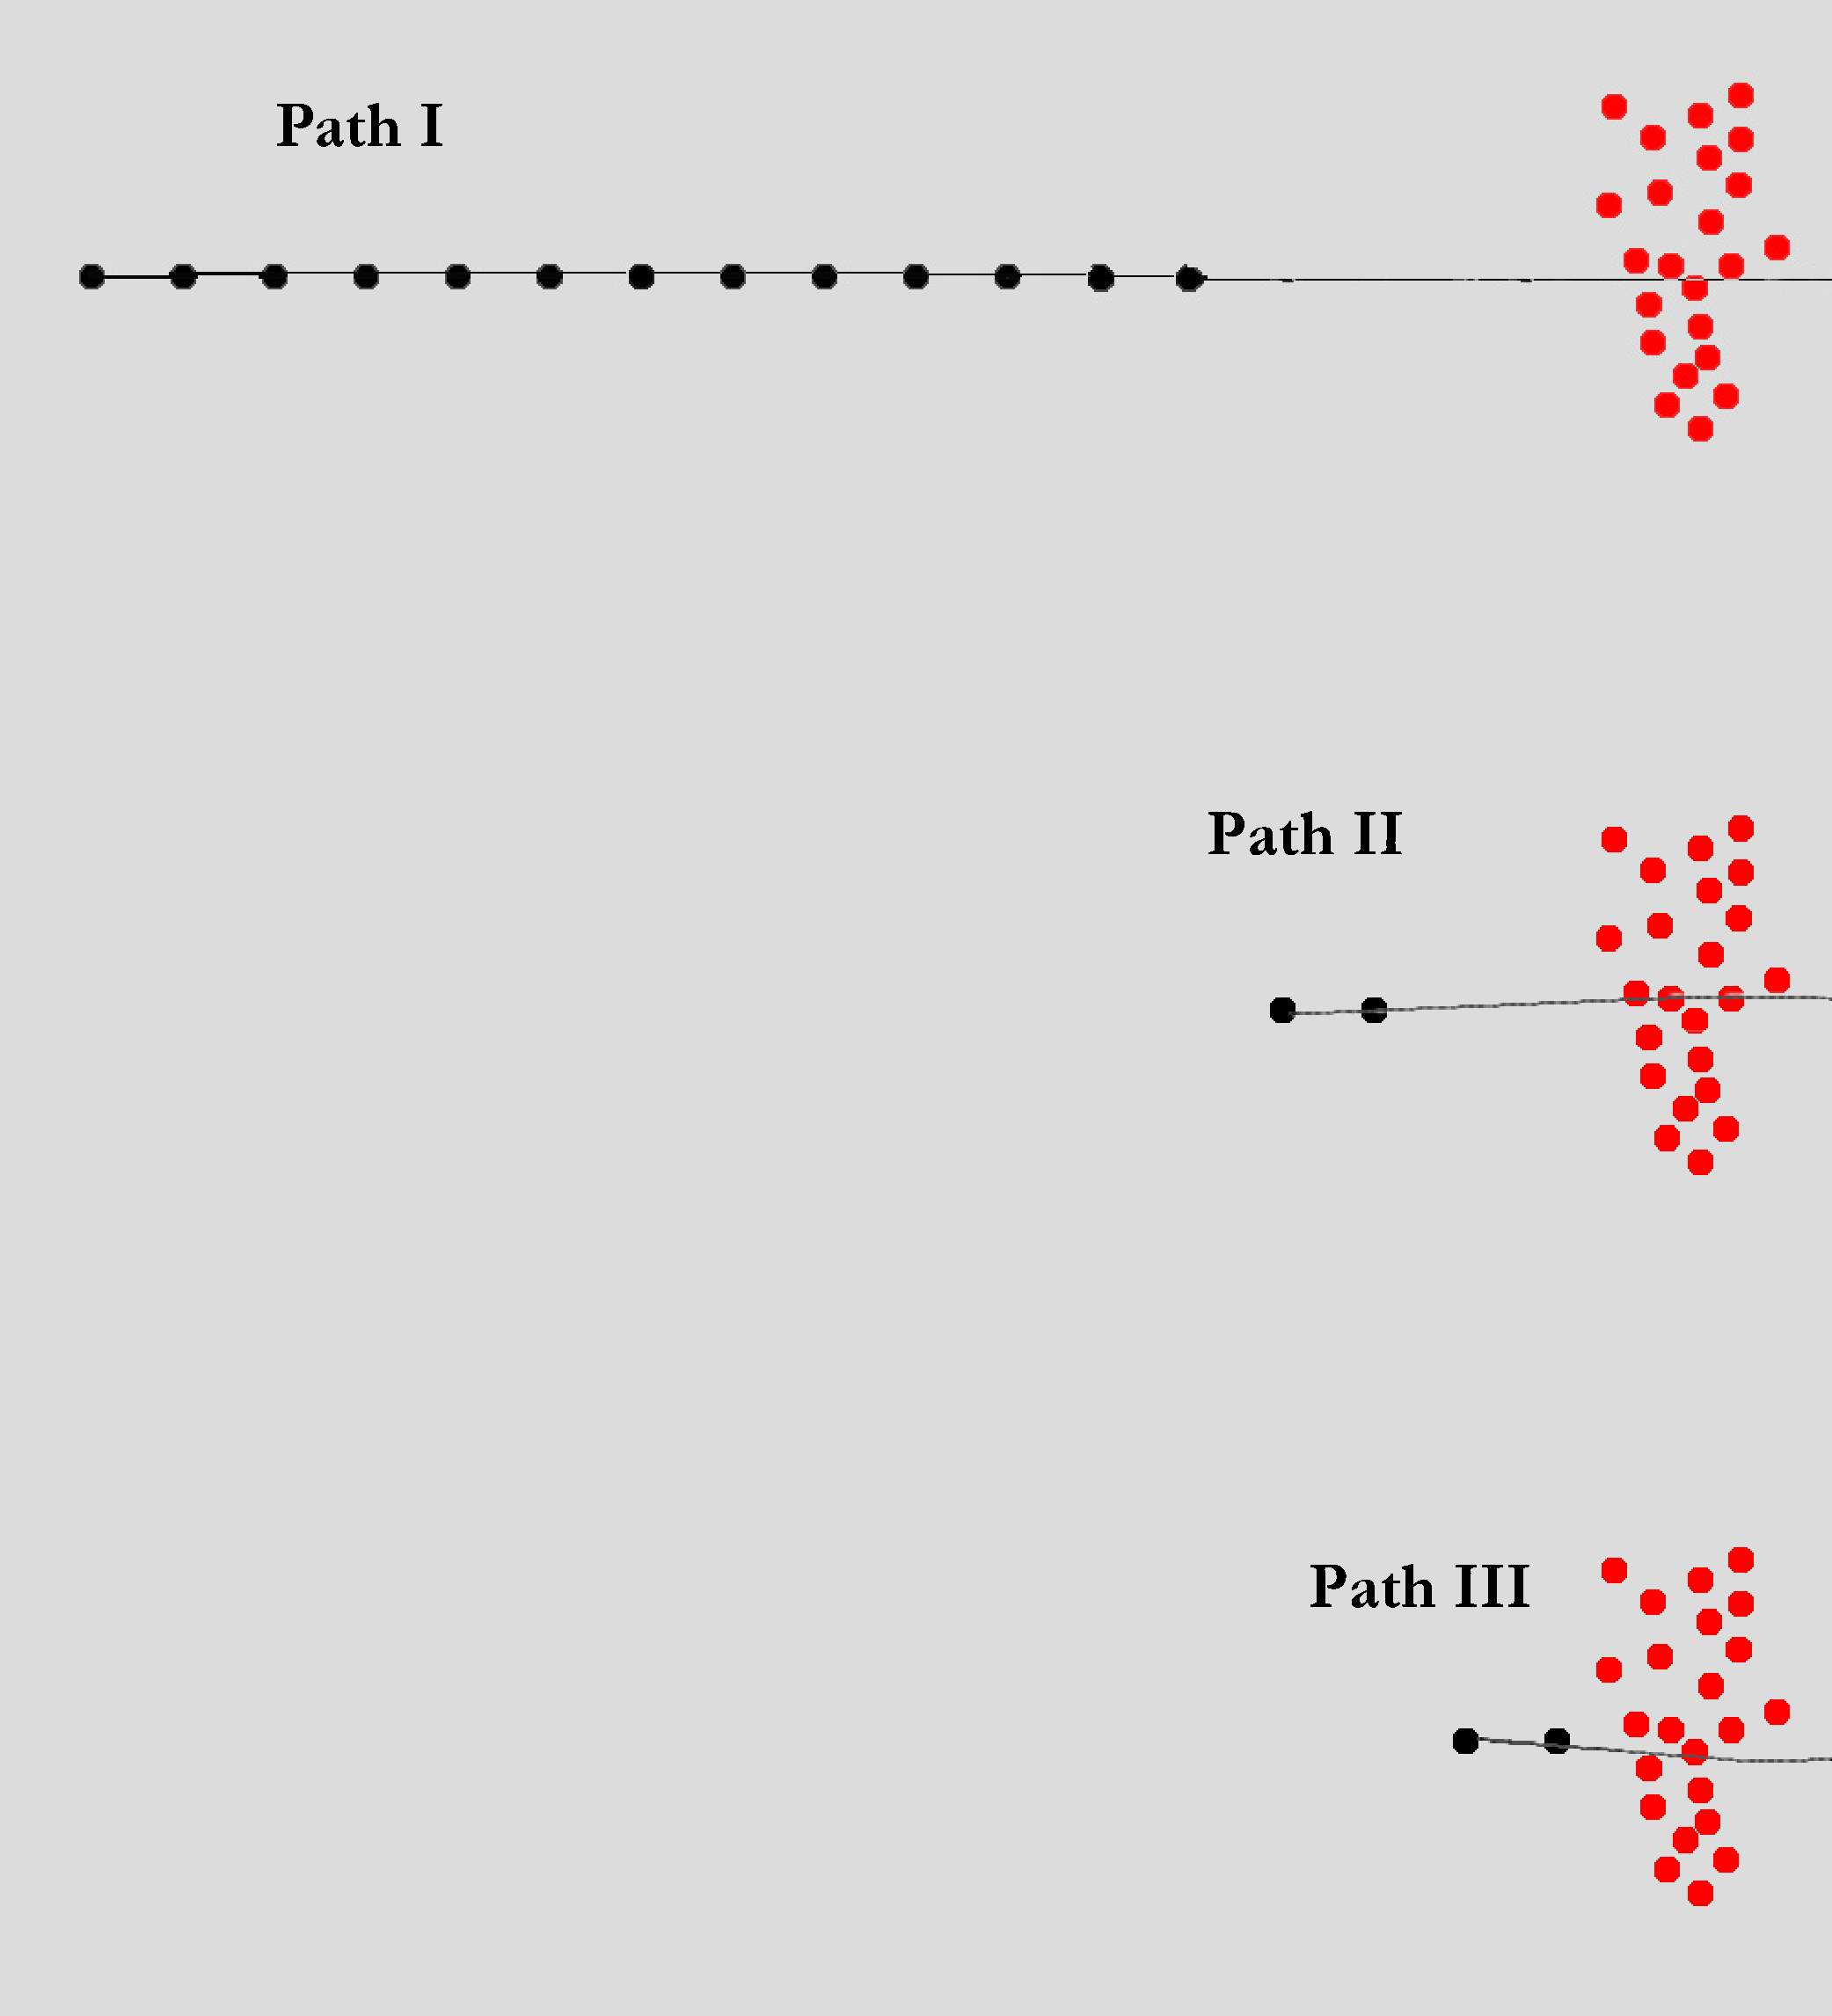
\includegraphics[width=7.5cm,height=12cm]{InfoBasedPerception/Exp2_RVO2}}
   \hspace{1pt}
  \subfloat[Using Group Based Perception]{\label{Exp2_GBP}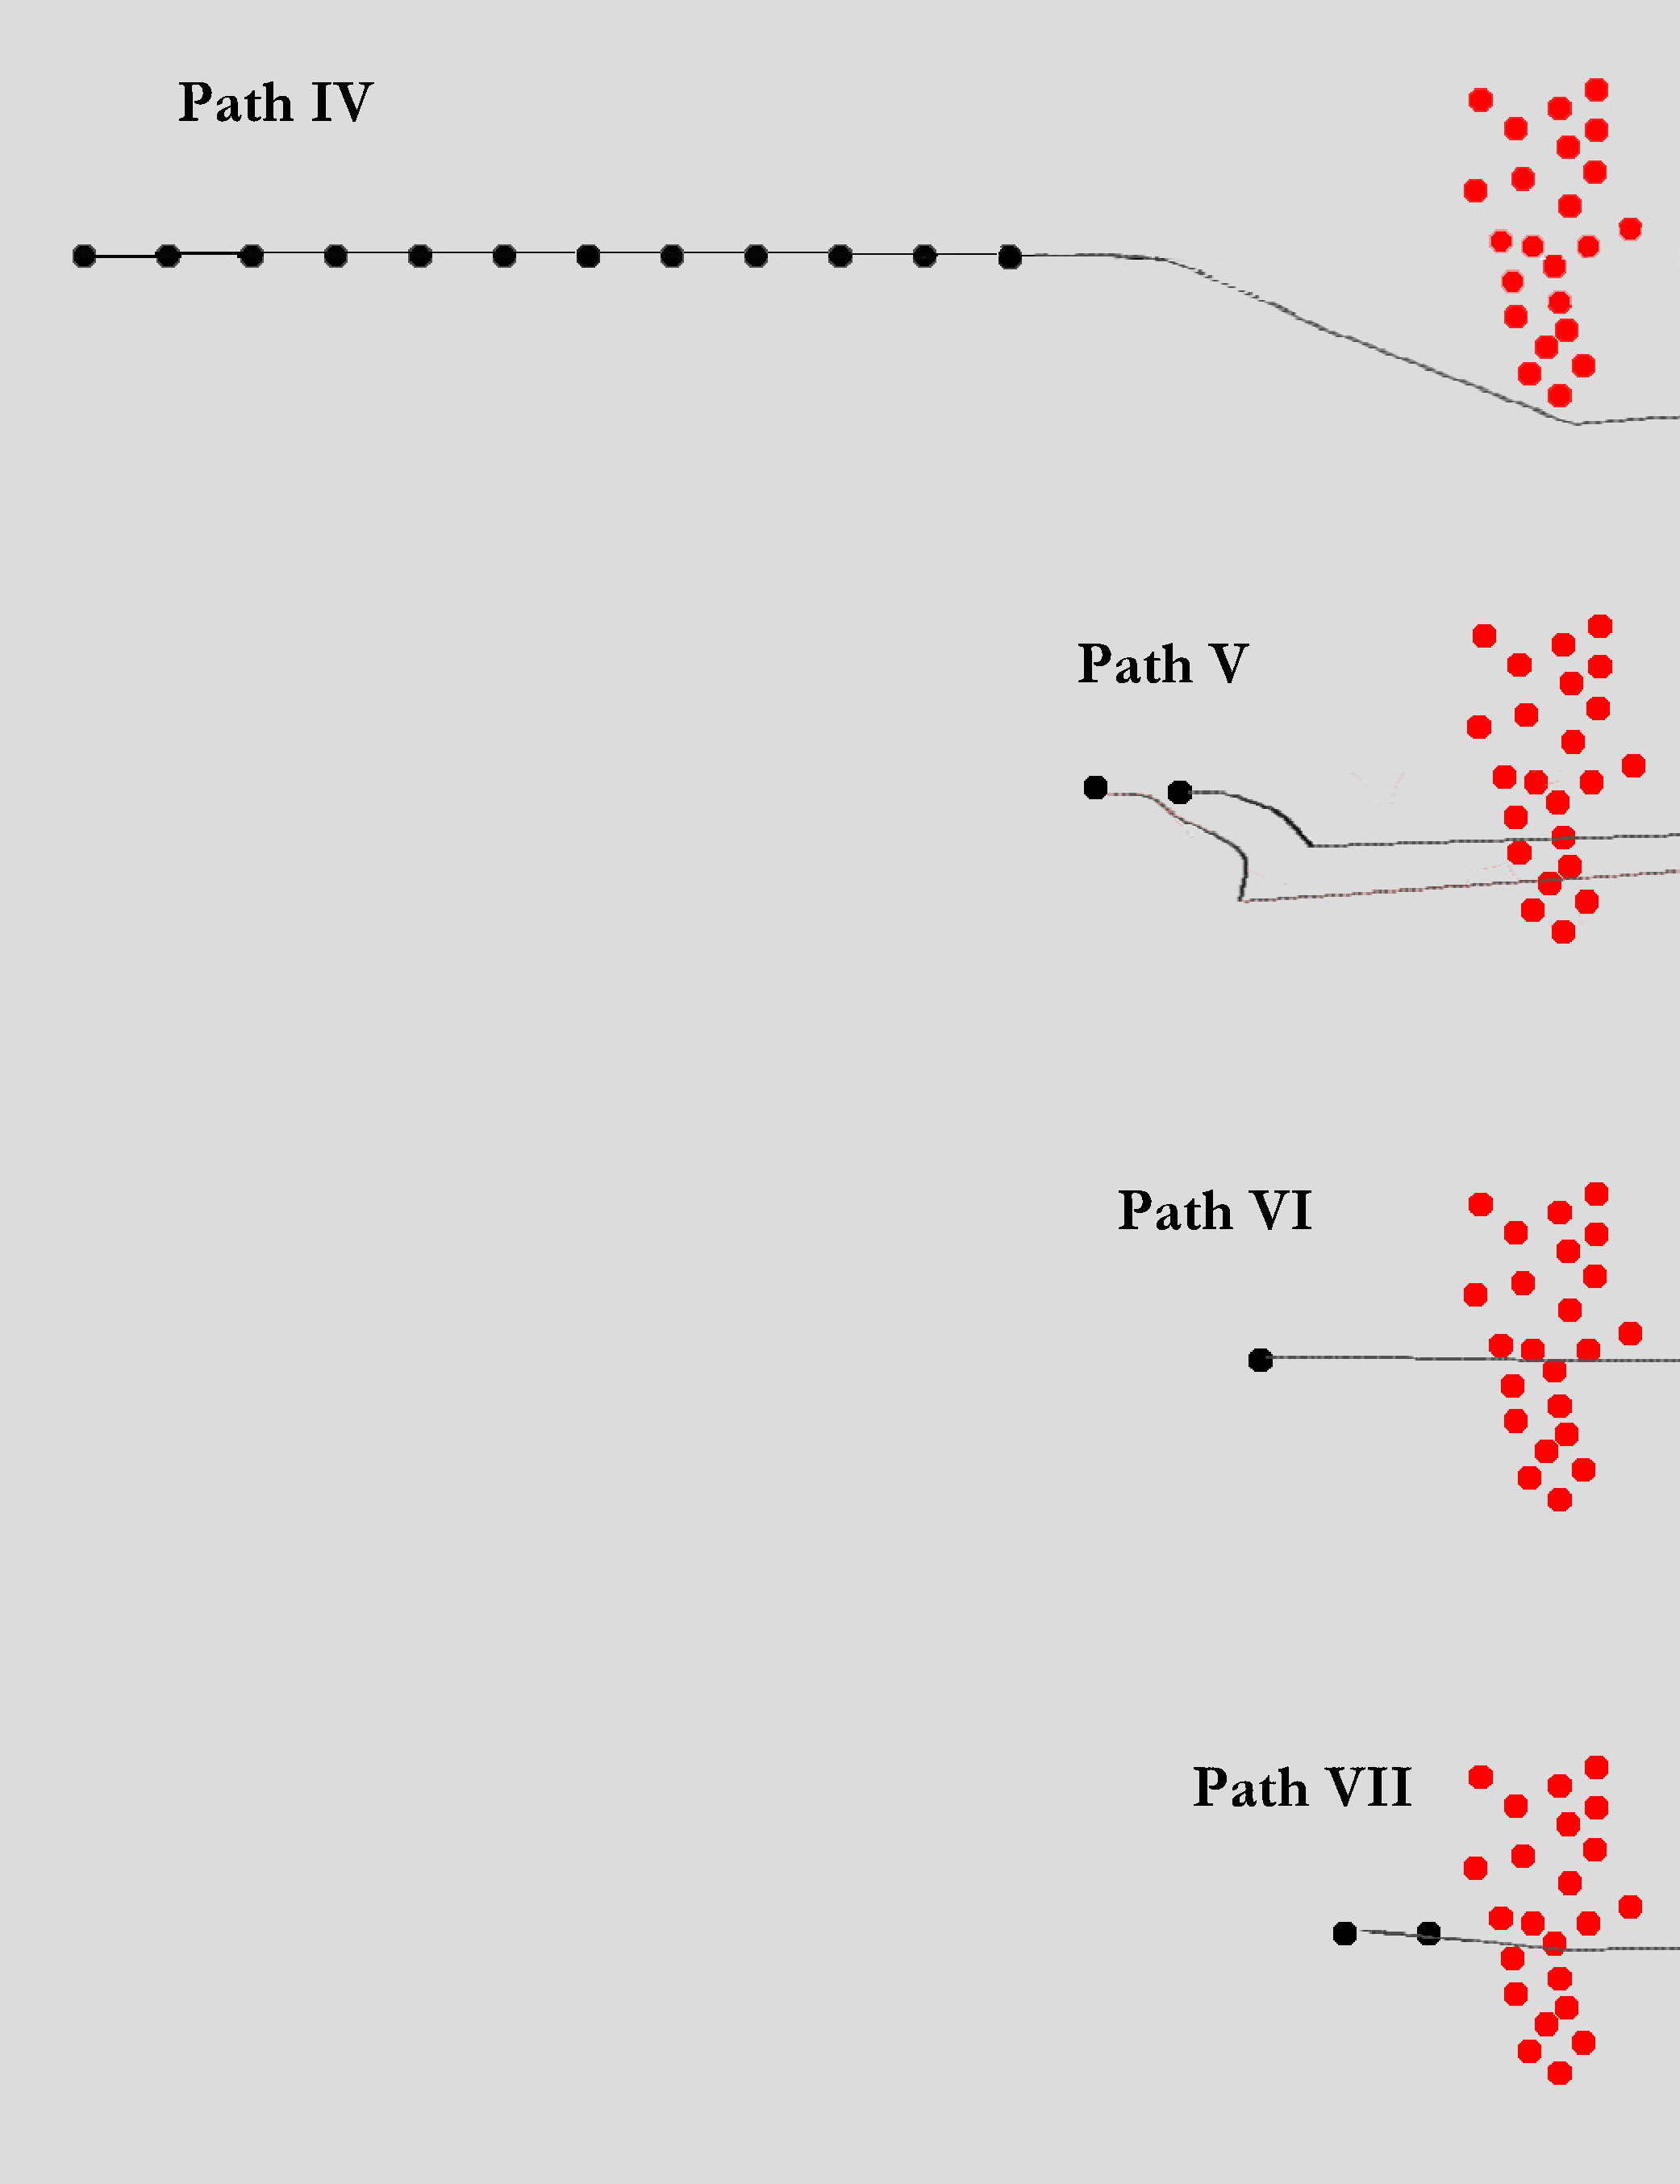
\includegraphics[width=7.5cm,height=12cm]{InfoBasedPerception/Exp2_GBP}}
  \caption{Experiment 2: Effect of multi layered clustering}
  \label{Exp2}
\end{figure}

In this experiment, the simple scenario where a single (black) agent had to get past a big group of agents to get to its goal is studied. The same experiment was performed by keeping the agent at different distances from the group. The objective of this experiment is two-fold. Firstly, it demonstrates the importance and the working of the multi-layered clustering (Section~\ref{IBP:Sensing}) used. Secondly, it demonstrates that when agents are very close to each other, where RVO2 already performs well, the Group Based Perception does not interfere with RVO2's functioning.

To recap, the multiple layers are used to describe groups of varying size at varying ranges of perception. This means agents will perceive other agents as groups or individuals depending on the distance; as an agent moves towards a group it will start to perceive the group as individual agents.

When GBP isn't used, the path followed does not change significantly with distance. The agents in the path of the black agent, give way to the agent, and the black agent just proceeds straight through the center of the large group (Path I in Fig.~\ref{Exp2_RVO}). In the last few cases (Paths II and III), the path is slightly different because the black agent does not have enough time to plan for a smooth, straight path and hence there is a slight deviation. Also, similar to the experiment in Section~\ref{GBP} it is forced to slow down in the process.

The result produced when GBP is used is more varied. Four distinctly different paths (labeled IV, V, VI and VII in Fig.~\ref{Exp2_GBP}) are produced based on how far the oncoming black agent is from the big group. At distances between 7-18m away from the center of the big cluster, the agent has enough time to perceive the group and avoid it completely (Path IV). At distances between 5-7m away, due to the size of the group, the agent gets too close to the group such that it then perceives the group as individuals. At this time (as described in Fig.~\ref{fig:ClusterLayer}) the agent performs motion planning on all the individual agents and as a consequence moves through the group, shown by path V. Path VI is obtained in a similar fashion; however, the black agent is too close to the group (4m away) to discern the effect of GBP. At distances closer than this (2-3m away), the path followed by the agent (Path VII) is exactly the same as that followed by the agent not using Group Based Perception (Path III). We argue that this type of flexibility in the perception of groups is critical to creating more natural behavior, humans will adapt what they perceive based on success or failure of their attempt to avoid larger groups.

\begin{figure}[!t]
  \centering
   \subfloat[Black Agent- Effort]{\label{Exp2_Black_Effort}\includegraphics[width=7.5cm,height=5cm]{InfoBasedPerception/Exp2_Black_Effort}}
  \hspace{1pt}
    \subfloat[Black Agent- Decision Inconvenience]{\label{Exp2_Black_decision_inconvenience}\includegraphics[width=7.5cm,height=5cm]{InfoBasedPerception/Exp2_Black_inconvenience}}
  \\
  \subfloat[Remaining Agents- Effort]{\label{Exp2_Remaining_Effort}\includegraphics[width=7.5cm,height=5cm]{InfoBasedPerception/Exp2_Remaining_Effort}}
  \hspace{1pt}
  \subfloat[Remaining Agents- Decision Inconvenience]{\label{Exp2_Remaining_decision_inconvenience}\includegraphics[width=7.5cm,height=5cm]{InfoBasedPerception/Exp2_Remaining_inconvenience}}
  \caption{Experiment 2: Quantitative Analysis}
  \label{Exp2_QuantitativeAnalysis}
\end{figure}

Figures~\ref{Exp2_Black_Effort} and \ref{Exp2_Remaining_Effort} show a comparison of the effort expended by the black agent and the average effort expended by all the remaining agents while using a traditional sensor range and GBP. As in the previous experiment (Section~\ref{GBP}) there is hardly any difference in the effort expended in both scenarios (except for a slight increase for path V). However, an interesting pattern can be observed in the decision inconvenience measurement (Figures~\ref{Exp2_Black_decision_inconvenience} and \ref{Exp2_Remaining_decision_inconvenience}). Firstly, the decision inconvenience for the rest of the group, is always lesser when GBP is used and almost the same for the black agent when path IV is followed. However, when path V or VI is followed there is a spike in the decision inconvenience curve. This can be explained by considering the fact that in both path V and VI, the black agent changes its planned path suddenly and decides to go through the group, thus not only increasing its own decision inconvenience but also the decision inconvenience caused to others in the group who have to move to give way to the agent. Finally, when path VII is followed both the effort and decision inconvenience count are exactly the same as for path III.

\subsubsection{Filtering necessitates Group Based Perception}


\begin{figure}[!t]
  \centering
  \subfloat[Initial Scenario]{\includegraphics[height=5cm]{InfoBasedPerception/Exp3_initial}}
   \\
    \subfloat[Info limit of 4, without GBP]{\label{Exp3_4_RVO}\includegraphics[width=7.5cm,height=4cm]{InfoBasedPerception/Exp3_4_RVO}}
    \hspace{1pt}
   \subfloat[Complete knowledge, without GBP]{\label{Exp3_full_RVO}\includegraphics[width=7.5cm,height=4cm]{InfoBasedPerception/Exp3_full_RVO}}
  \\
  \subfloat[Info limit of 1, with GBP]{\label{Exp3_1_GBP}\includegraphics[width=7.5cm,height=4cm]{InfoBasedPerception/Exp3_1_GBP}}
  \hspace{1pt}
  \subfloat[Info limit of 4, with GBP]{\label{Exp3_4_GBP}\includegraphics[width=7.5cm,height=4cm]{InfoBasedPerception/Exp3_4_GBP}}
  \caption{Experiment 3: The necessity of Group Based Perception}
  \label{Exp3}
\end{figure}

In Section~\ref{IBP:Theory}, the fact that humans have limited information processing capacity was explained. In this experiment, it is demonstrated that if a human being's limited information processing capability is to be modeled, it is necessary to use Group Based Perception. This is done by observing the simple scenario of an agent moving towards two groups of other agents (Fig.~\ref{Exp3}). When no information limit is imposed on the agent, and a normal circular sensor range is used, the agent, as expected, follows a nice straight path through the center of the group. However, when an information limit of $il_a = 4$ is imposed on the agent, the black agent, does not perceive all the individual agents in the group and  as a result it is forced to reconsider its path mid-route. As a result, the irregular trail shown in Fig.~\ref{Exp3_4_RVO} is obtained. However, in the same situation, when Group Based Perception is used, the agent smoothly avoids the whole group (Fig.~\ref{Exp3_4_GBP}). In fact, this smooth path is obtained for as low a limit as $il_a = 1$ (Fig.~\ref{Exp3_1_GBP}).

\subsubsection{Effect of filtering of percept information}

The final experiment (Fig.~\ref{Exp4}) demonstrates the effect of filtering, i.e.\ having limits on the information processing capabilities of the agents. The scenario consists of an agent moving towards a collection of individuals (moving towards the agent) followed by a group of agents behind the set of individuals. In the first case an information limit of $il_a = 5$ is set so that the agent is continually capable of perceiving a larger number of other agents and groups. In the second scenario a lower limit of $il_a = 3$ is used such that the agent isn't initially capable of perceiving the group behind the individuals. Figure~\ref{Exp4_5_1} shows how agents perceive the cluster that is farther away, even when there is an immediate collision to avoid. Figure~\ref{Exp4_5_2} shows that the agent manages to move around this group because it had a head start in planning - i.e.\ , it considered the group early when avoiding collisions. In the second scenario it could process a maximum of 3 or 4 percepts at any given time because of the lower information limit. Due to this, as seen in Fig.~\ref{Exp4_3_1}, the agent cannot see beyond the immediate obstacles in front and does not prepare in advance to avoid the larger group. Once the agent finally perceives this group, it is too late to move around this group as it perceives the group as individuals and then moves through the group as in Fig~\ref{Exp4_3_2}.


\begin{figure}[!tb]
  \centering
   \subfloat[Initial Scenario]{\includegraphics[height=5cm]{InfoBasedPerception/Exp4_initial}}
   \\
   \subfloat[InfoLimit 3: Step 1]{\label{Exp4_3_1}\includegraphics[width=7.5cm,height=4cm]{InfoBasedPerception/Exp4_3_1}}
  \hspace{1pt}
    \subfloat[InfoLimit 5: Step 1]{\label{Exp4_5_1}\includegraphics[width=7.5cm,height=4cm]{InfoBasedPerception/Exp4_5_1}}
  \\
  \subfloat[InfoLimit 3: Step 2]{\label{Exp4_3_2}\includegraphics[width=7.5cm,height=4cm]{InfoBasedPerception/Exp4_3_2}}
  \hspace{1pt}
  \subfloat[InfoLimit 5: Step 2]{\label{Exp4_5_2}\includegraphics[width=7.5cm,height=4cm]{InfoBasedPerception/Exp4_5_2}}
  \caption{Experiment 4: Effect of filtering of percept information}
  \label{Exp4}
\end{figure}

This experiment illustrates how small differences in the information limit can generate different forms of behavior in the agents. Interestingly, the info limit of 3 and 5 correspond to Cowan's finding~\cite{Cowan:2001wi} that all humans can cognitively process only 3-5 chunks of information at any given time. Clearly the value of the limit is critical to behavior, it is also proposed that this limit will change with personal characteristics and the emotional state of the agents. In fact this varying limit of perception may be an important factor for collisions in actual crowds, this is especially relevant in emergency egress scenarios where stress and collisions are critically important to safety planning. We plan to attempt to quantify this information limit through experimentation in future work.


In this section, we demonstrated the capabilities and the usefulness of the Information Based Perception system in Motion Planning by analyzing the effect of group based perception, multi-layered clustering and the filtering of information. In the next section, we demonstrate that RVO2 when used with IBP produces results that are at least as good as with a traditional sensor range by analyzing its performance in standard scenarios.

\subsection{Validation against standard scenarios} % (fold)
\label{sec:validation_against_standard_scenarios}

Several studies have identified standard scenarios against which motion planning systems have to be validated empirically. Hu~\cite{hunanThesis} classified these scenarios based on their main motion axes (\emph{mma}) into three main categories. Based on this categorization, he identified that validation against scenarios with 1, 2 and greater than 2 \emph{mmas} would be necessary to validate a model. In this section, we demonstrate that in these three standard scenarios, IBP enhanced RVO2 produces motion similar to traditional RVO2. For a more detailed discussion on the setup of these scenarios and the reason for this categorization, the reader is directed to Hu's thesis~\cite{hunanThesis}.
% section validation_against_standard_scenarios (end)

\subsubsection{Corridor (1 \emph{mma})} % (fold)
\label{sec:corridor}

Hu et al.~\cite{hunanThesis} identified a corridor with agents starting at either end and moving towards each other as the standard scenario in this category. Figure~\ref{fig:standard_corr} illustrates the simulation results produced by RVO2 with a traditional simple circular sensor range against RVO2 with a Group Based Perception system. An empirical observation of the simulation results does not seem to indicate much difference between the two models.


\begin{figure}[!t]
    \centering
        \subfloat[IBP - $10$ seconds]{\label{standard_corr_ibp_1}\includegraphics[width=7.5cm]{InfoBasedPerception/corr-IBP-2}}
            \hspace{1pt}
        \subfloat[RVO2 - $10$ seconds]{\label{standard_corr_rvo_1}\includegraphics[width=7.5cm]{InfoBasedPerception/corr-RVO-2}}
            \\
        \subfloat[IBP - $15$ seconds]{\label{standard_corr_ibp_2}\includegraphics[width=7.5cm]{InfoBasedPerception/corr-IBP-4}}
            \hspace{1pt}
        \subfloat[RVO2 - $15$ seconds]{\label{standard_corr_rvo_2}\includegraphics[width=7.5cm]{InfoBasedPerception/corr-RVO-4}}
                \\
        \subfloat[IBP - $17.5$ seconds]{\label{standard_corr_ibp_3}\includegraphics[width=7.5cm]{InfoBasedPerception/corr-IBP-5}}
            \hspace{1pt}
        \subfloat[RVO2 - $17.5$ seconds]{\label{standard_corr_rvo_3}\includegraphics[width=7.5cm]{InfoBasedPerception/corr-RVO-5}}
        \\
        \subfloat[IBP - $20$ seconds]{\label{standard_corr_ibp_4}\includegraphics[width=7.5cm]{InfoBasedPerception/corr-IBP-6}}
            \hspace{1pt}
        \subfloat[RVO2 - $20$ seconds]{\label{standard_corr_rvo_4}\includegraphics[width=7.5cm]{InfoBasedPerception/corr-RVO-6}}
    \caption[Corridor Experiment Screenshots]{Corridor Experiment: Scenario with 1 main motion axis. With IBP, the lane formation is slightly more asymmetric}
    \label{fig:standard_corr}
\end{figure}
% section corridor (end)

Traditionally, in this scenario, it is expected that the pedestrian agents form lanes to handle the counter flow and prevent jamming~\cite{PhysRevE.85.066128}; this is seen in both models in Figure~\ref{fig:standard_corr}. Based on more detailed studies done in~\cite{PhysRevE.85.066128}, Hu et al. suggested several qualitative measurements of the lane formation phenomenon. Firstly, they observed that lanes with a longer lifetime can more reliably reduce jams and disordered flow. As seen in the figure, both models simulated seem to produce lanes that last the length of the simulation. They also suggested that, due to the pedestrians'�� anticipation, lanes start to form early. As Figure~\ref{standard_corr_ibp_1} illustrates, with group based perception, the agents at the edges starts forming lanes even earlier than traditional RVO2 does. \cite{PhysRevE.85.066128} also stated that two or three asymmetric lanes are more realistic than a larger number of symmetric lanes. The simulations seem to indicate that when IBP
 is used, the lanes produced by the RVO2 agent become more asymmetric and arguably more realistic.

Thus, it can be seen that, in this scenario, RVO2 with IBP qualitatively produces results that are at least as good as traditional RVO2. This is further confirmed by the average effort expended calculation shown in Table~\ref{tab:energy} where both models have similar values. The effort expended was calculated as in Section~\ref{sec:model_demonstration}, using Equation~\ref{eq:energyEquation}.

\subsubsection{Intersection (2 \emph{mma})} % (fold)
\label{sec:cross}

In this category, the typical scenario identified is an intersection of two corridors with groups of pedestrians crossing each other at the intersection. Figure~\ref{fig:cross} illustrates the results of the simulation. The figure indicates that group based perception does not make much difference in this scenario. Lanes are similarly formed in both scenarios with most agents passing through smoothly. However, due to the group based perception, the efficiency and symmetry of this movement is somewhat reduced with one agent being dragged out of its preferred path by the other group because it initially tries to avoid the group. However, the calculation of the average effort per person shown in Table~\ref{tab:energy} indicates that this is not that significant a difference. Moreover, it is difficult to argue which of the two results are more accurate without experimental data.

\begin{figure}[!tp]
    \centering
        \subfloat[RVO2+IBP-200 seconds]{\label{standard_cross_ibp_1}\includegraphics[width=4.9cm]{InfoBasedPerception/cross-IBP-1}}
            \hspace{1pt}
        \subfloat[RVO2+IBP-250 seconds]{\label{standard_cross_ibp_2}\includegraphics[width=4.9cm]{InfoBasedPerception/cross-IBP-2}}
            \hspace{1pt}
        \subfloat[RVO2+IBP-300 seconds]{\label{standard_cross_ibp_3}\includegraphics[width=4.9cm]{InfoBasedPerception/cross-IBP-3}}
            \\
        \subfloat[RVO2+IBP-350 seconds]{\label{standard_cross_ibp_4}\includegraphics[width=4.9cm]{InfoBasedPerception/cross-IBP-4}}
            \hspace{1pt}
        \subfloat[RVO2+IBP-400 seconds]{\label{standard_cross_ibp_5}\includegraphics[width=4.9cm]{InfoBasedPerception/cross-IBP-5}}
            \\
        \subfloat[RVO2-200 seconds]{\label{standard_cross_rvo_1}\includegraphics[width=4.9cm]{InfoBasedPerception/cross-RVO-1}}
            \hspace{1pt}
        \subfloat[RVO2-250 seconds]{\label{standard_cross_rvo_2}\includegraphics[width=4.9cm]{InfoBasedPerception/cross-RVO-2}}
             \\
        \subfloat[RVO2-300 seconds]{\label{standard_cross_rvo_3}\includegraphics[width=4.9cm]{InfoBasedPerception/cross-RVO-3}}
             \hspace{1pt}
        \subfloat[RVO-350 seconds]{\label{standard_cross_rvo_4}\includegraphics[width=4.9cm]{InfoBasedPerception/cross-RVO-4}}
    \caption[Intersection Experiment Screenshots]{Intersection Experiment: IBP seems to marginally reduce the efficiency with which collisions are avoided in this scenario. However, this is the case only for one agent.Moreover, it is difficult to determine which result is more accurate.}
    \label{fig:cross}
\end{figure}
% section corridor (end)



\subsubsection{Circle (multiple \emph{mma})} % (fold)
\label{sec:circle}

The third and final category identified in~\cite{hunanThesis} was also the most complicated in that there are several mmas. The scenario considered to best represent this category is one with 32 agents in a circular formation. Each agent tries to exchange positions with the agent diametrically opposite to it. Collision avoidance algorithms, like RVO2, are expected to smoothly navigate this situation without a deadlock developing. For IBP to be practical, it is expected that IBP does not adversely affect the effectiveness with which RVO2 handles this difficult scenario. As shown by the trails in Figure~\ref{fig:circle} and Table~\ref{tab:energy}, this is indeed the case. Despite the trails produced being different in some ways, deadlocks do not appear and the average total effort per person is only marginally higher when IBP is used.


\begin{figure}[!t]
    \centering
        \subfloat[RVO2+IBP]{\label{circle_ibp_1}\includegraphics[scale=0.5]{InfoBasedPerception/circle32-IBP-RVO2}}
            \\
        \subfloat[RVO]{\label{circle_ibp_2}\includegraphics[scale=0.5]{InfoBasedPerception/circle32-RVO2}}
    \caption[Circle Experiment Screenshots]{Circle Experiment: IBP does not have a significant impact on the results produced by RVO2 in this scenario. Unnatural deadlocks do not develop in either scenario.}
    \label{fig:circle}
\end{figure}
% section corridor (end)


\begin{table}[!t]
\label{tab:energy}
\centering
%     \begin{adjustbox}{width=\textwidth,center}
    % \begin{adjustbox}{center}
        \begin{tabular}{p{2in}   p{2in}   p{2in} p{2in}}
                \hline
            \multicolumn{1}{c}{Model} &\multicolumn{1}{p{1.2in}}{Corridor (kJ/person)} &\multicolumn{1}{p{1.2in}}{Intersection (kJ/person)} &\multicolumn{1}{p{1.2in}}{Circle (kJ/person)}   \\
                \hline
                \hline
            \multicolumn{1}{l}{IBP+RVO2} & \multicolumn{1}{l}{152.725} & \multicolumn{1}{l}{141.183}& \multicolumn{1}{l}{115.802}
            \\%\cline{2-5}
                \hline
            \multicolumn{1}{l}{RVO2} & \multicolumn{1}{l}{152.355} & \multicolumn{1}{l}{141.193}& \multicolumn{1}{l}{111.207}
                \\%\cline{2-5}
                \hline
                \hline
        \end{tabular}
%     \end{adjustbox}
%     \vspace{ - 05 mm}
    \caption[Table summarizing effort expended for standard scenarios]{This table shows the average energy expended per agent in standard scenarios and compares the results of RVO2 with traditional sensing against RVO2 with IBP. There seem to be no significant differences between the models by this measure.}
\end{table}



In this section, we have demonstrated the working of RVO2 using IBP by comparing it against the RVO2 with a traditional sensor range in three standard scenarios: bi-directional corridor, a two-corridor intersection and a circle scenario. IBP produced results that were at least as good as a traditional sensor range in all three scenarios. In the next section, we validate the proposed model against real world data.

\subsection{Experimental validation} % (fold)
\label{sec:experimental_validation}

The experiments so far discussed in this section, have been based on quantitatively and qualitatively analyzing simulations in different scenarios. However, to better validate the model and the theory of group collision avoidance on which it is based it would be necessary to compare it against real world data. Hu et al.~\cite{HuNan2013,hunanThesis} conducted a series of controlled field experiments to study the interaction among individual participants and their movement in certain scenarios. In this section, the experimental setup used by Hu in his thesis is first reproduced. Following this, the results obtained are presented and compared against the results produced by RVO2 agents using Information Based Perception.

\subsubsection{Experiment setup} % (fold)
\label{sec:experiment_setup}

This section explains the experimental setup and measurements made by Hu et al. to study human movement in particular scenarios\footnote{This section simply summarizes the experiments conducted by Hu et al. to provide a context for the subsequent analysis and validation done. For a more detailed discussion please refer to the original paper and thesis.}. In the original paper three experiments were conducted, since IBP does not produce results different from the underlying motion planning algorithm used (RVO2 in this case) for two of the scenarios only the first experiment analyzing movement of pedestrians walking towards each other is presented and considered in this analysis.

\begin{figure}[!t]
    \begin{center}
        \includegraphics[width=\textwidth]{InfoBasedPerception/schematic_setup.pdf}
    \end{center}
    \caption[Schematic of layout of experiment area~\cite{hunanThesis}.]{A 13.5 m x 2.5 m area is demarcated for the experiments. The participants stand 10m apart and are directed to walk towards the other end at their prefered speed. (From~\cite{hunanThesis})}
    \label{fig:schematic_setup}
\end{figure}


The experiments were conducted at an outdoor passage outside the School of Computer Engineering in Nanyang Technological University. Figure~\ref{fig:schematic_setup} shows the setup of the experiment. Each experiment consisted of three participants (marked 1, 2 and 3) moving at their preferred speed in the given direction until they reached the goal point marked by the border of the demarcated area. Hu et al argue that this scenario is typical of several real life bi-directional movement scenarios. In order to shift attention from movement, the participants were given some simple algebraic calculations to do as they move.  The experimental setup is shown in Figure~\ref{fig:detailed_setup}. A video camera with adequate resolution was kept at fixed height above the experimental area using a horizontal tripod. The location of the camera and the lens was fixed to ensure maximum clarity and minimal distortion. Markers were kept on the experimental area to prevent participants from going outside the experimental area and to help in analysis of results obtained. Participants were also asked to wear white helmets so that the analysis from the video was accurate~\cite{W:2004tp}.


\begin{figure}[!tbhp]
    \begin{center}
        \includegraphics[]{InfoBasedPerception/detailed_setup.pdf}
    \end{center}
    \caption[Actual setup of Nan's experiments~\cite{hunanThesis}]{The experimental setup used by Hu et al.~\cite{hunanThesis} for their controlled field experiments.}
    \label{fig:detailed_setup}
\end{figure}

Videos of 20 experiments with 13 participants (9 male; 4 female) were finally analyzed for characteristic movement patterns and other metrics. The process shown in Figure~\ref{fig:the_video_extraction_process} was then used to extract the trajectories of each of the participants in each of the recorded videos. Briefly, the process was as follows: first the video was converted into a series of images at 20 frames per second which is an ideal frame rate to obtain a complete trajectory of the movement of participants. Once an image stack was obtained the image was scaled, rotated and transformed using the markers to remove distortions and bring it to metric scale. Following this, the next two steps quantize the image and remove noise such that, at the end of the process, each image only has black and white colors with the former depicting the background and the latter the participants. Lastly, an existing software is used for tracking each participant (white particle) in the quantized images. Fig.~\ref{fig:VideoExtractionExample} gives an example of the whole process.

\begin{figure}[!tb]
    \begin{center}
        \includegraphics[scale=0.75]{InfoBasedPerception/DataExtractionProcess.pdf}
    \end{center}
    \caption{The data extraction process.}
    \label{fig:the_video_extraction_process}
\end{figure}

\begin{figure}[!htb]
    \centering
   		\subfloat[Step 1]{\includegraphics[width=7.5cm,height=4cm]{InfoBasedPerception/extract_1}}
  		\hspace{1pt}
    	\subfloat[Step 2]{\includegraphics[width=7.5cm,height=4cm]{InfoBasedPerception/extract_2}}
  		\\
  		\subfloat[Step 3]{\includegraphics[width=7.5cm,height=4cm]{InfoBasedPerception/extract_3}}
  		\hspace{1pt}
  		\subfloat[Step 4]{\includegraphics[width=7.5cm,height=4cm]{InfoBasedPerception/extract_4}}
  		\\
  		\subfloat[Step 5]{\includegraphics[width=7.5cm,height=4cm]{InfoBasedPerception/extract_5}}
  		\hspace{1pt}
  		\subfloat[Step 6]{\includegraphics[width=7.5cm,height=4cm]{InfoBasedPerception/extract_6}}
  	\caption{An example of the video extraction process}
    \label{fig:VideoExtractionExample}
\end{figure}





\subsubsection{Quantitative measurements of experimental data} % (fold)
\label{sec:metrics_used}

\begin{figure}[!hb]
    \begin{center}
        \includegraphics[width=\textwidth]{InfoBasedPerception/CategoriesPicture}
    \end{center}
    \caption{The trajectories of participants can be grouped into 3 categories}
    \label{fig:categoriesOfMotion}
\end{figure}

The data extraction process outlined in Section~\ref{sec:experiment_setup} produces for each participant in each experiment a trajectory. Trajectories that were similar were grouped together and normalized to find an average trajectory for each group. It was observed that these trajectories could be grouped into three main groups shown in Figure~\ref{fig:categoriesOfMotion}.  The quantitative measurements that are explained next are all calculated on the average trajectory for each of these groups.

The different measurements used by Hu et al. are very neatly summarized in Figure~\ref{fig:OverviewOfMetrics}. These metrics are:

\begin{figure}[!htb]
    \begin{center}
        \includegraphics[width=\textwidth]{InfoBasedPerception/metricsUsedHuNan}
    \end{center}
    \caption{Metrics proposed by Hu et al. for quantitative validation of models~\cite{hunanThesis}.}
    \label{fig:OverviewOfMetrics}
\end{figure}

\begin{itemize}
    \item Trajectory length of participant $i$ ($L_i$).
    % \item Distance deviated from the horizontal direction line (along the x axis) of participant $i$ as a function of time $t$ ($dd^t_i$). The horizontal direction line is also the shortest trajectory for the participant towards his goal.
    \item Maximum deviation of participant $i$ ($D_i$). This is the maximum value of $dd^t_i$ for a participant over the course of the complete trajectory.
    % \item  The local curvature of participant $i$ as a function of time ($lc^t_i$). The local curvature of a participant at a given time is the tangent of the angle formed by the instantaneous velocity of the participant to the velocity along the horizontal direction line.
    % \item The difference of local curvatures between participants $i$ and $j$ as a function of a time $t$ ($\Delta lc^t_{ij}$).
    \item The speed of the participant as function of time $t$ ($s^t_i$).
    \item The distance between agents $i$ and $j$ as a function of time $t$ ($d^t_{ij}$).
\end{itemize}

% section metrics_used (end)


\subsubsection{Results and comparison} % (fold)
\label{sec:comparison_of_ibp}

This section presents the simulation results produced using IBP when compared against the experimental data. The experimental setup was replicated by initializing the agents as shown in Fig.~\ref{fig:experiment_simulation_setup}. Of the four metrics proposed, the maximum deviation and inter-agent distance against time seemed to differentiate best between the models. Hence, in this section, we use these metrics for evaluating IBP. Appendix~\ref{cha:speed_experiment_comparison} discusses briefly the results of the other two metrics.

\begin{figure}[!b]
    \begin{center}
        \includegraphics[width=\textwidth]{InfoBasedPerception/expSimulationSetup}
    \end{center}
    \caption[Layout of experiment in simulation]{The initial configuration of the simulation based on the experimental setup in real world experiments.}
    \label{fig:experiment_simulation_setup}
\end{figure}


% The metrics in Section~\ref{sec:metrics_used} can be broadly grouped into two kinds: temporal measures and non-temporal ones.

Table~\ref{tab:RealWorldDistanceDeviation} shows the maximum deviation values for the real world data. It can be broadly seen that in $95\%$ of the cases, Participant 2 avoided Participant 1 and 3 through either side. It can also be seen that the major deviation effort was taken by single agent ($\approx 0.87m$) rather than the group of two agents ($\approx 0.2 -0.3m$). Table~\ref{tab:IBPDistanceDeviation} compares the distance deviation calculation for the simulation results against the real world data. Due to the symmetry of the behavior of agents 1 and 3 in category 1 and 2 of the real world experiments, we do not loose much information by averaging category 1 and 2 to obtain the values in the second column of Table~\ref{tab:IBPDistanceDeviation} which represents 95\% of the real world data. The remaining columns in the same table show the results produced by traditional RVO2, Social Force and RVO2 with IBP.  As can be seen, RVO2 with IBP produces the dynamics most similar to the real world experiments. This is more clearly illustrated in Figure~\ref{fig:nonTemporalIllustration}.


\begin{table}[!t]

\centering
%     \begin{adjustbox}{width=\textwidth,center}
    % \begin{adjustbox}{center}
        \begin{tabular}{p{0.75in}   p{0.75in} p{0.75in} p{0.75in}}
            \hline
            \multicolumn{4}{c}{Maximum Deviation Calculation from Experiments}  \\
            \hline
            \multicolumn{1}{c}{} &\multicolumn{1}{c}{Category 1 (\textbf{55\%})} &\multicolumn{1}{c}{Category 2 (40\%)}  &\multicolumn{1}{c}{Category 3 (5\%)} \\
            \hline
            \hline
            \multicolumn{1}{l}{Agent 1} & \multicolumn{1}{l}{0.0785} & \multicolumn{1}{l}{0.320723} & \multicolumn{1}{l}{0.241166}
            \\%\cline{2-5}
            \multicolumn{1}{l}{Agent 2} & \multicolumn{1}{l}{\textbf{0.8720}}& \multicolumn{1}{l}{\textbf{0.868398}}& \multicolumn{1}{l}{0.320865}
            \\%\cline{2-5}
            \multicolumn{1}{l}{Agent 3} & \multicolumn{1}{l}{0.2656}& \multicolumn{1}{l}{0.18667}& \multicolumn{1}{l}{\textbf{0.657496}}
                                    \\
            \hline
            \hline
        \end{tabular}
%     \end{adjustbox}
%     \vspace{ - 05 mm}
    \caption[Real world maximum deviation~\cite{hunanThesis}]{This table summarizes the maximum deviation according to experiments conducted by Hu~\cite{hunanThesis}. Category 1 refers to the movement of Agent 2 to the left of the group, category 2 to the movement of Agent 2 to the right of the group and category 3 to the movement of agent 2 through the middle of the oncoming group.}
    \label{tab:RealWorldDistanceDeviation}
\end{table}

\begin{table}[!b]
\label{tab:SimulationDistanceDeviation}
\centering
%     \begin{adjustbox}{width=\textwidth,center}
    % \begin{adjustbox}{center}
        \begin{tabular}{ p{0.75in}   p{0.75in} p{0.75in} p{0.75in} p{0.75in}}
            \hline
             \multicolumn{1}{c}{} & \multicolumn{1}{c}{Experiment (95\%)} & \multicolumn{1}{c}{IBP-RVO2} & \multicolumn{1}{c}{RVO2} & \multicolumn{1}{c}{Social Force}    \\
            \hline
            \hline
             \multicolumn{1}{l}{Agent 1} & \multicolumn{1}{l}{0.199} & \multicolumn{1}{l}{0.0} & \multicolumn{1}{l}{0.043} & \multicolumn{1}{l}{0.372}
            \\%\cline{2-5}
            \multicolumn{1}{l}{Agent 2}  & \multicolumn{1}{l}{\textbf{0.870}} & \multicolumn{1}{l}{\textbf{0.855}} & \multicolumn{1}{l}{\textbf{0.003}} & \multicolumn{1}{l}{\textbf{0.0}}
            \\%\cline{2-5}
            \multicolumn{1}{l}{Agent 3}  & \multicolumn{1}{l}{0.226} & \multicolumn{1}{l}{0} & \multicolumn{1}{l}{0.038} & \multicolumn{1}{l}{0.372}\\
            \hline
            \hline
        \end{tabular}
%     \end{adjustbox}
%     \vspace{ - 05 mm}
    \caption[Maximum deviation measurements from simulations]{This table shows the trajectory length obtained for the simulation of the experimental scenario in~\cite{hunanThesis}. The first column lists the average of category 1 and 2 which together comprised 95\% of the real world experiment data of~\cite{hunanThesis}. The same pattern of agent 2 having larger value than the other two is obtained only when IBP is used.}
    \label{tab:IBPDistanceDeviation}
\end{table}

\begin{figure}[!t]
    \begin{center}
        \includegraphics[width=0.75\textwidth]{InfoBasedPerception/maxDevIllustration}
    \end{center}
    \caption{Graphical illustration of the  absolute difference in maximum deviations that can be seen in Table~\ref{tab:energy}.}
\end{figure}

Figure~\ref{fig:DistanceIBPPlot} illustrates the inter-agent distance as a function of time for the experimental data, RVO2, Social Force and RVO2 with IBP. As in the real world experiments of Hu it can be seen that agents 1 and 3 maintain a relatively constant value. It can also be seen that, at its closest point, as in the experiment, agent 2 becomes closer to one of agent 1 and 3 than they are to each other. This is closer to the experimental data than the results produced by RVO2 and Social Force using a normal sensor range as shown in Fig.~\ref{fig:DistanceIBPPlot-RVO2} and Fig.~\ref{fig:DistanceIBPPlot-SF}.

\begin{figure}[!tb]
  \centering
  \subfloat[Experiment- Category 1 (55\%)~\cite{hunanThesis}]{\includegraphics[width=0.48 \textwidth]{InfoBasedPerception/interAgentDistanceCat1}}
  \hspace{1pt}
  \subfloat[Experiment- Category 2 (40\%)~\cite{hunanThesis}]{\includegraphics[width=0.48 \textwidth]{InfoBasedPerception/interAgentDistanceCat2}}\\
   \subfloat[IBP-RVO2]{\label{fig:DistanceIBPPlot-IBP}\includegraphics[width=0.6\textwidth]{InfoBasedPerception/DistancePlot-RVO2-IBP}}
\\
   \subfloat[RVO2]{\label{fig:DistanceIBPPlot-RVO2}\includegraphics[width=0.6\textwidth]{InfoBasedPerception/DistancePlot-RVO2}}
\\
    \subfloat[Social Force]{\label{fig:DistanceIBPPlot-SF}\includegraphics[width=0.6\textwidth]{InfoBasedPerception/DistancePlot-SocialForce}}
  \caption[Inter agent distances over time.]{Plot of inter agent distances over time for various models and the experimental data.}
  \label{fig:DistanceIBPPlot}
\end{figure}

Thus, this section has demonstrated how Information Based Perception helps RVO2 produce results that are  similar to those obtained by Hu et al. in their controlled experiments.


% section experimental_validation (end)

\section{Summary and Future Work}
\label{IBP:Conclusion}

We began this chapter with an argument that traditional spatial distance based perception systems limited the ability of existing motion planning systems to produce realistic motion.
An Information Based Perception model for agents which is based on perceived information rather than spatial distance was introduced based on existing theories of human cognition. Through simulations and comparison against real world experiments it was argued that this is a more appropriate model of human perception for crowd and egress simulation as it helped produce more realistic group avoidance behavior. The idea that humans have limited perception capacity such that they only process certain obstacles more relevant to collision avoidance was incorporated and its usefulness demonstrated. The real world experiments conducted by Hu et al. were introduced and comparison of simulation results against experimental results showed that Information Based Perception can help models like RVO2 replicate the results produced by the experiments.



The IBP model can be extended so that during filtering it can recognize cues that contain event and environment information as well. This can be passed as input to the Event Identification system which is described in more detailed in Chapter~\ref{chapter:PreEvacuationBehavior}. Also, one aspect of the model that has not been explored much is the quantification of information limits and appropriate definitions of interest; real world experiments could be conducted to attempt to quantify these parameters. The third criteria which was mentioned in Section~\ref{IBP:Filtering}, i.e.\ the inherent interestingness of perceived objects, could also be the subject of these real world experiments.

In emergency situations, according to Ozel~\cite{Ozel:2001tn}, humans start perceiving cues in the environment differently. The idea of modelling different cues and their effect on the agent's information processing capabilities as suggested by Kuligowski~\cite{Kuligowski:2009un} is an idea that will be discussed in more detail in Chapter~\ref{chapter:PreEvacuationBehavior}. As mentioned by Hill~\cite{Hill:1999ww} there is also a reciprocal effect of cognition on perception where agents would turn towards objects of more interest. These could also be incorporated into a later version of the IBP model. In the next chapter, a model for how perceived cues can be used for identifying events and modelling pre-evacuation behavior is presented.


    %!TEX root = vaisagh_thesis.tex

\chapter{Modelling Pre-evacuation Behavior}
\label{chapter:PreEvacuationBehavior}


Ideally, when a fire starts a fire alarm goes off; all occupants hear this alarm and use the nearest safe exit to leave the building. However, this is hardly the norm. In many cases, occupants are desensitized from hearing false alarms and often do not start to evacuate until they are completely sure that egress is necessary. On January 19, 2000, a fire in Boland Hall in Seton Hall University killed three students because they had ignored the fire alarms assuming they were false~\cite{Berry:2000us}. This uncertainty about the authenticity of the first sign of danger isn't an isolated incident~\cite{Graham:2000vl,Proulx:2001we,Proulx:1995wq,Proulx:2003tc,Purser:2001ts,Ramachandran:1990wj,Sime:1995uu,Tong:1985wn}. This delay in reaction time of evacuees can have a huge impact on existing plans for egress if it is not taken into consideration. Thus, it is important to consider this when developing evacuation plans. In other words, when studying the behavior of evacuees, it is necessary to study and understand their actions from the time at which the fire started right up until the point where the last person evacuated~\cite{Tong:1985wn}.



As discussed in Chapters~\ref{chapter:LiteratureReview} and~\ref{chapter:IBEVAC}, pre-evacuation uncertainty and investigation are features of human behavior during egress that are rarely considered in existing models. To recap, \emph{pre-evacuation} refers to the period of time that elapses after the start of the fire alarm before the person starts evacuating. While some models~\cite{Tsai:2011tz} do have a simplified model of pre-evacuation behavior, they fail to model it in enough detail to enable their extension to more general cases. For example, a fire alarm could have different effects based on the clarity and believability of the alarm~\cite{Kobes:2009jx,Paulsen:1984ti}. This variability is hard to simulate in existing models of pre-evacuation behavior. Also, during an evacuation people exchange event and environment related information with others. Evacuees are unlikely to follow every message that they receive blindly. There is a variability in the \emph{trust} in messages received that can have different effects on egress. This is rarely considered in existing models.


In this chapter, we present a model for simulating pre-evacuation behavior and event identification\footnote{This model was presented at the Pedestrian and Evacuation Dynamics Conference in 2012 and appeared in print in 2014~\cite{Viswanathan:2012vt}.}. In the model, the evacuees identify and process information in terms of event cues which exist throughout the environment. Section~\ref{PreEvac:LitRev} first explores some of the existing work that motivates the need to model pre-evacuation behavior. Following this, Section~\ref{PreEvac:EventIdentification} explains the proposed model and, finally, Section~\ref{PreEvac:Results} illustrates through experimentation the usefulness of this model, the importance of modelling pre-evacuation behavior and having a communication model.



\section{Related Work}
\label{PreEvac:LitRev}


As discussed in Section~\ref{LiteratureReview:CurrentUnderstanding}, there are a lot of conflicting theories on how humans behave in emergencies and why they behave as they do. However, there are certain behaviors that are fundamental to human nature and are generally accepted as fact, such as the constant search for information~\cite{Proulx:2003tc,Tong:1985wn,Ozel:2001tn,Sime:1983uy}. This section first summarizes the existing knowledge of human behavior during egress with special emphasis on pre-evacuation behavior. Following this, some existing models of pre-evacuation behavior and evacuee communication are presented.

\subsection{On modelling pre-evacuation behavior}
\label{PreEvac:PreEvacuationBehavior}

Several studies of human behavior during emergency egress~\cite{Kuligowski:2005tt,Ozel:2001tn,Proulx:2007ul}, have shown that an evacuee's first reaction after realizing that there is an unusual situation is to investigate and gather more information about the situation. Evacuation starts only once the need for evacuation is established. \emph{Cues} are the key to understanding this transition from realization to investigation and, eventually, to evacuation.

Cues are certain changes in the environment that indicate that something is wrong or different from normal~\cite{Sime:1983uy}.
They come in different forms. Fire and smoke are the typical and most effective cues for an evacuation. Fire alarms and people running or instructing to escape are also cues. According to Sime~\cite{Sime:1983uy}, there are three kinds of cues:
\begin{itemize}
\item Ambiguous Cues: E.g. Hearing noises or shouting, or seeing someone run.
\item Verbal Cues: E.g. Instructions from a companion, announcement from the stage.
\item Unambiguous Cues: E.g. Seeing smoke or fire, or seeing someone run with a fire extinguisher.
\end{itemize}


According to some researchers~\cite{Ramachandran:1990wj,Proulx:2007ul}, an ambiguous cue by itself does not cause a person to initiate investigation. Rather, the cue has to persist for a period of time before investigation begins and results in the finding of an unambiguous cue. Interestingly, according to Tong and Canter~\cite{Tong:1985wn}, even unambiguous cues don't result in people immediately exiting the building, rather it initiates a complicated process consisting of information searching and affiliation.

The effect of cues and the evacuee's reaction to it depends on many factors. The identity of an individual's primary group and its proximity and availability determines the reaction of a person to a cue~\cite{Sime:1983uy}. In~\cite{Latane:1969wm} an experiment was conducted where particpants were placed in a room with smoke; the experiment showed that when alone, 75 percent of the subjects reported the smoke. However, in the presence of two non-reacting others only 10 percent of the subjects reported the smoke during the experimental period.

Various studies~\cite{Proulx:2003tc,Proulx:2001we,Paulsen:1984ti,Sandberg:1997tw,Cocking:2008vv,Tong:1985wn} emphasize the importance of the location and the person's role in the significance of cues. As an example, a fire alarm at home is more likely to cause a person to act than a fire alarm at their office, which will most likely be considered a false alarm. People's societal role determines their training and responsibility and thus their alertness to cues and the preparedness for reacting to it.

Their groups, location and environment aren't the only factors that influence people's behavior during evacuation. There are also a lot of \emph{intrinsic factors} that influence how people react to fires. What these factors are and how influential they are are a matter of much debate. Over the years there have been several surveys~\cite{Tong:1985wn,Sandberg:1997tw,Kuligowski:2009un} that discuss these intrinsic factors.

Andr\'{e}e and Eriksson's report~\cite{Andree:2008td} even had a cross cultural study that compared the evacuation behavior of Swedish students against the behavior of Australian students. Except for grouping behavior they found few significant differences in the behavior during evacuations. Kobes et al., in their survey~\cite{Kobes:2009jx}, compared some studies of evacuation behavior from the USA, Great Britain and Australia and commented on them being ``identical in their essence''. Some factors like age and gender were found to not significantly affect pre-evacuation behavior. A person's social role is one of the commonly accepted factors that influence evacuation behavior~\cite{Sandberg:1997tw,Kobes:2009jx,Paulsen:1984ti}. Factors like the person's experience with fires, training, disabilities, familiarity with the environment, etc.\ are accepted to have a great influence on pre-evacuation behavior.

Close to a hundred different studies on human behavior in fires were used by Kuligowski~\cite{Kuligowski:2009un} to compile a list of the factors that influence egress and more specifically pre-evacuation behavior. In this article, she suggests that the period that we term as \emph{pre-evacuation} itself consists of two phases. Phase 1 is called \emph{perception}; The idea being that the existence of a cue does not guarantee its perception. The Table~\ref{tab:Cues} lists some factors that can affect this perception of a person and whether these factors increase or decrease the chance of the person perceiving the abnormality in the situation.

Kuligowski calls the next phase \emph{interpretation}. During this phase, the person searches for more information to verify whether a fire has actually started and if it actually poses a threat that needs to be handled. Many studies~\cite{Ozel:2001tn,Proulx:2007ul} have confirmed the importance of this phase, though sometimes they are known by different names. In~\cite{Ozel:2001tn} this phase is called \emph{unconflicted inertia} to indicate how the person either continues what he's doing or tries to finish of his activity without actually beginning to evacuate. In~\cite{Tong:1985wn}, this phase is called \emph{investigation} to indicate the search for information that enables the interpretation of the system. Regardless of what it is called, this phase consists of two parts:
\begin{inparaenum}
\item defining the situation as a fire and
\item defining the risk that the situation poses.
\end{inparaenum}


Kuligowski categorized the factors that influence these phases into two types: occupant based factors~(which are equivalent to the intrinsic factors mentioned earlier) and cue based factors. These factors and their effects are shown in Table~\ref{tab:Cues}. Increases/Decreases signifies a cues effect on that particular phase. Also, cue based factors, do not simply consist of events, but also their nature and features.


% Requires the booktabs if the memoir class is not being used
\begin{table}[htbp]
\centering
\begin{threeparttable}[b]
\topcaption{Factors affecting Evacuation Behavior.] The list of factors affecting evacuation behavior and their influences as presented in Kuligowski's survey~\cite{Kuligowski:2009un}} % requires the topcapt package
\begin{tabular}{m{6.3cm} c >{\centering\arraybackslash}m{2.8cm} >{\centering\arraybackslash}m{2.8cm}} % Column formatting, @{} suppresses leading/trailing space
\toprule
Factors & Perception  & 2a: Definition of the Situation as a Fire & 2b: Definition of the Risk to Self/Others\\

\midrule
\multicolumn {4}{l}{{\bf Occupant-based pre-event factors}}\\
\midrule
Has experience with fires    & Increases  & Increases &  Increases\\
Has knowledge of fire/ training & Increases  & Increases &  Increases\\
Habituation with environment   & Decreases  & ---\tnote{1}    &  --- \\
Has knowledge of routes     &   ---   &  ---    & Decreases\\
Has frequent experience with false alarms & ---  & Decreases &  ---\\
Has a feeling of security in the building & ---  & Decreases &  ---\\
Has perceptual disability   & Decreases  & --- &  ---\\
Is older adult        & Decreases  & --- &  Increases\\
Is woman           & Increases  & --- &  Increases\\
Speaks the same language as others & Increases  & --- &  ---\\
Has frequent interaction with family & Increases  & --- &  ---\\
\midrule
\multicolumn {4}{l}{{\bf Occupant-based event factors}}\\
\midrule
Has a higher stress/ anxiety level  & Decreases & --- & --- \\
Perceives a time pressure & Decreases & Decreases & Increases \\
Presence of others~(especially loved ones) & Decreases & --- & Increases \\
Proximity to fire / Visual Access  & Increases & --- & --- \\
Sleeping & Decreases & ---& ---\\
A higher number of behavioral processes(>1) & --- & Increases & --- \\
Defines situation as a fire & -- & N/A & --- \\
\midrule
\multicolumn {4}{l}{{\bf Cue-based factors}}\\
\midrule
A higher number of cues & Mixed\tnote{2} & Increases & Increases \\
Consistent cues & --- & Increases & Increases \\
Unambiguous cues & --- & Increases & --- \\
Social cues~(others' actions) that are consistent with an understanding of a fire situation & --- & Increases & Increases \\
Official source & Increases & Increases &---\\
Familiar source & --- & Increases &--- \\
A higher dose of toxic gases & --- & Decreases & --- \\
Extreme/ dense cues & Decreases & --- & Increases \\
Visual/ audible cues & Increases & --- & --- \\
Risk Information & --- & Increases & --- \\
\bottomrule
\end{tabular}
\begin{tablenotes}
\item[1]{Areas where no research is found is marked by ---}
\item[2]{Research conflicted on the direction of influence of this factor}
\end{tablenotes}
\label{tab:Cues}
\end{threeparttable}
\end{table}



One of the factors that encourage the programmatic implementation of cue based factors is the fact that the effect of a cue can be explained to be caused by the nature and characteristics of the cue rather than the specific cue. In other words, each cue can be described in terms of its ambiguity, consistency with other cues and its source and it is this description that determines the effect of the cue.


\subsection{Existing models}
\label{PreEvac:ExistingModels}

There are very few existing models that take pre-evacuation period into consideration. Pre-evacuation decision making of an individual was modeled by Pires~\cite{Pires:2005gs} using a simple Bayesian Belief Network~(BBN).

Fran{\c c}a et al.~\cite{Franca:2009wq} created a simulation model of the development of panic behavior during emergency egress. This model implemented the hysterical belief theory~\cite{Torres:2010tj} and modeled how panic first develops and then evacuation happens. It also had a basic communication system through which agents exchanged mood information (which is a key factor in the development of panic) by using the grid based environment as a medium for communicating messages. Despite pre-evacuation behavior being modeled in some detail, it is not possible to extend this model to replicate the heterogeneity in people's reaction to cues.

ESCAPES~\cite{Tsai:2011tz} is a model that takes into account some factors like the spread of knowledge, fear and emotion between the different evacuees. These factors are used to create a simplistic model of pre-evacuation behavior. Effectively though, only the \emph{perception} part of pre-evacuation behavior is modeled. This means that  once an agent perceives a cue i.e. another agent running, the perceiving agent immediately starts to evacuate.

The event identification and communication model proposed in this chapter have been influenced by these models. However, it is unique in the way that the diversity of cues and their effects can be considered; and more importantly, in how both the perception and investigation phase of pre-evacuation behavior can be simulated in this computational model. Data on pre-evacuation behavior is difficult to gather: If participants are given prior warning like in fire drills, their behavior is likely to be unrealistic; on the other hand, not giving prior warning could be risky and dangerous. Thus, in this chapter, the proposed models are validated against established theories.

\section{A Bucket Model of Event Identification}
\label{PreEvac:EventIdentification}

% First explain how cues are modeled
Section~\ref{PreEvac:PreEvacuationBehavior} discussed how ambiguity, source and consistency of the cue~\cite{Kuligowski:2005tt,Sime:1983uy,Tong:1985wn} are the key factors in determining the effect of a cue. This is the fundamental idea used in the proposed model. Ambiguity refers to the clarity of the cue. A cue that gives a clear signal of an event would be unambiguous while an ambiguous cue will lack this clarity. For example, a traditional ringing fire alarm is highly ambiguous while the modern fire alarms with voice updates are much less ambiguous and they have different effects on pre-evacuation behavior. The source of a cue is also important; there is a clear difference in perceived danger in a situation when the warning is given by figure of authority like a fire marshal as opposed to an unknown stranger. Lastly, if the signals given by cues are inconsistent then it would take longer for a person to start egress. For example, if no other occupant is perceived to be raising an alarm or trying to evacuate, most people would not react to smoke~\cite{Latane:1969wm}.

Each cue is located at a particular location $(x,y)$ in the environment and is sensed by agents when within their perception range. When a cue is sensed, an agent obtains a certain amount of information $\mu$ about the current state of the world. Thus, a cue in the Bucket model is represented as a tuple $(\mu, x, y)$ where $\mu$ is the amount of information obtained from the cue and $(x,y)$ is the location of the cue. When an event or an action of significance occurs at some location a cue is created at that location.


Once perceived, these cues are processed by the agent's Event Knowledge System which manages the information from cues. The Event Knowledge System has two \emph{buckets}  of information: one corresponding to \emph{investigation ($\beta_{i}$)} and the second corresponding to \emph{egress ($\beta_{e}$)}. When a cue is perceived, a certain amount of information ($\mu_{\beta_{i}}$ and $\mu_{\beta_{e}}$) is added to the respective bucket(s) based on the ambiguity level, consistency and source of the cue.  For each bucket, a \emph{threshold} ($\tau_{\beta_{i}}$ and $\tau_{\beta_{e}}$) is initially fixed  based on the intrinsic characteristics of the agent. When the amount of information in a bucket overflows the threshold the agent changes its internal state and proceeds towards a new goal based on the behavior model that is used. For the purpose of the experiments in this chapter, each agent has three states that it can be in: \emph{normal} behavior where the goal is the center of the \emph{starting} room of the agent; \emph{milling} behavior where the agent gathers with other agents at the nearest \emph{corridor} (See Figure~\ref{fig:layout}); and \emph{evacuation} where the agent heads towards the exit through the shortest route. Figure~\ref{fig:stateTransitions} illustrates the working of the bucket model within this simple behavior model.

\begin{figure}[!t]
    \begin{center}
        \includegraphics[width=0.65\textwidth]{EventIdentification/stateTransitions}
    \end{center}
    \caption[An illustration of the bucket model]{An illustration of the bucket model and the behavior model of agents used in the experiments. Each cue adds (or removes) a certain amount of information $\mu$ to one or both buckets ($\beta_{i}$ and $\beta_{e}$). An overfilling bucket causes a state transition.}
    \label{fig:stateTransitions}
\end{figure}

There are two sets of values here which have been mentioned: bucket thresholds ($\tau$) and the amount of information ($\mu$) that a cue contributes. As mentioned earlier, each cue is characterized by its consistency, ambiguity and source. Cues that indicate a need to egress have $\mu > 0$ and add information to buckets while cues that do not, remove information from it (i.e. $\mu<0$). Thus if an inconsistent set of cues are observed at a given time, less or maybe even no information might be added to each bucket.

The amount of information that is added or removed (i.e. the value of $\mu$) depends on the ambiguity and source of the cue. The key value in the \emph{bucket model} is the ambiguity of the cue. Each cue has an ambiguity value that is represented as a real number in the range $[0,1]$. Since each cue adds or removes information from the \emph{investigation} and \emph{egress} buckets, there are two information values associated with each cue, one for each bucket.

In theory, the amount of information added by a cue can be any decreasing function of the ambiguity of the cue. For simplicity, we assume that it is a linear function with the value added by a cue of ambiguity $\alpha$ to the bucket $\beta$ being given by:
\begin{equation}
	\mu_{\beta} (\alpha) =
    \begin{cases}

        {\tau_{\beta}}{\left[1-\frac{(\alpha^{max}_{\beta}-\alpha)}{\alpha^{max}_{\beta}}\right]}^{-1} & \mbox{ if } \alpha \leq \alpha^{max}_{\beta}\\
        0 & \mbox{ if } \alpha > \alpha^{max}_{\beta}
    \end{cases} \mbox{where } \beta \in \{\beta_{i}, \beta_{e}\}
\end{equation}

Where $\tau$ is a constant equal to the egress bucket threshold value for a normal agent and is determined by the maximum time for the bucket to fill and the intrinsic characteristics of the agent. A higher value for $\tau$ would mean more information is added per cue and the bucket would fill faster. In terms of the formula, it simply determines the slope of the curve and the range of $\mu$.  We arbitrarily choose a value $10,000$ for $\tau$ so that the rate of change of $\mu$ for every $0.1$ unit change in ambiguity $\alpha$ is greater than $1$.

$\alpha^{max}_{e}$ refers to the maximum ambiguity level that has effect on the egress bucket which in this case is fixed at $0.9$ since we assume that cues more ambiguous than this do not add any information. This helps us simulate those cues that only result in investigation even if they persist for a long time and never trigger evacuation itself. % The formula above gives the relationship shown in figure~\ref{ambiguityInfoRelationship} between ambiguity level and time to start evacuation given a single cue of that ambiguity is perceived at each second.


A similar procedure is used to determine $\mu_{i}$. An ambiguity value of $1.0$ in this case represents a small amount of information, as opposed to no information in the case of the egress bucket. This is because even an unambiguous cue when perceived for long enough initiates investigation~\cite{Tong:1985wn}. Thus, $\alpha^{max}_{i} = 1.0$.

The value for threshold of each bucket is equal to $\tau$ for normal agents. For special agents, and to consider certain special scenarios and effects, we can simply choose a threshold $\tau^s < \tau$; this will be demonstrated in the experiments in Sections~\ref{sec:experiment_2_informed_and_informing_agents},~\ref{sec:experiment_3_modelling_the_effect_of_pre_evacuation_behavior} and~\ref{sec:experiment_4}.


% Following this explain how messages contain message cues and additional information.
The effect of the source of the cue is seen in the communication model. Communication is implemented as \emph{messages} sent from one agent to the other. Each message has a message cue and environment information. The message cue works just as other cues with it's own ambiguity level. Here the term ambiguity is used to refer to the trustworthiness of the source of the information. In the current version of the model, we use a simple communication mechanism whereby agents only exchange knowledge about the state of the fire, or more precisely the inaccessible parts of the map (those blocked by fire).

In the experiments in this chapter, a simple cellular automata based fire model and a simple finite difference smoke model are used to simulate the propagation of fire and smoke\footnote{Validated models of fire and smoke are not necessary for testing the proposed model- a plausible model is sufficient}. This creates fire and smoke cues at locations near the fire which spread as the simulation proceeds. The environment itself is made up of various rooms which are connected by links. Some rooms that link multiple rooms are marked as \emph{corridors} and are the gathering points for the agents when investigating. All agents are assumed to have complete spatial knowledge of the environment and are initially located in their \emph{starting} rooms. As soon as the fire starts, fire alarm cues are placed all over the environment. Agents react to these cues and mark observable pathways that are blocked as inaccessible in their spatial knowledge graph. Agents die immediately on contact with fire. Smoke, depending on the concentration, initially slows and eventually kills agents. All agents either escape or are killed at the end of the simulation.



% To recap the discussion in Chapter~\ref{chapter:IBEVAC}, the planning system of the agent on identifying a goal passes this goal to the Navigation System that proceeds through a three-level process to determine the preferred velocity of the agent. At the highest level, a logical path is determined in terms of rooms to be crossed from the agents current location to the goal. From this logical path, spatial way points or locations are extracted by the next level. The third and final level determines a possible collision free path to the farthest visible spatial waypoint. In the experiments in this chapter, A-Star is used for path planning and RVO2 is used for the motion planning system.


% Communication between agents is also modeled with agents being able to transmit messages within a fixed communication range.




\section{Results}
\label{PreEvac:Results}

% Outline what are the things that we expect to demonstrate
This section discusses the experiments that were conducted to demonstrate the effect that cue perception, pre-evacuation behavior and communication can have on egress. The simulations were conducted on the two floor office environment shown in Figure~\ref{fig:layout}. This was adapted from the first two floors of the World Trade Center in California.  Simulations were conducted with 200 agents randomly distributed over the two floors of the building and data was collected after averaging over 20 replications of the simulation.

\begin{figure}[!tbp]
\centering
\subfloat[Ground Floor]{\includegraphics[width= 0.9\textwidth]{EventIdentification/floor0}}
\\
\subfloat[Second Floor]{\includegraphics[width= 0.9\textwidth]{EventIdentification/floor1}}
\caption[The Environment Layout]{The two floors used for the simulation which is a modified version of the first two floors of the World Trade Center in California. The corridors, staircases and exits on both floors are marked. The numbers are the room numbers which are used in the experiments.}
\label{fig:layout}
% Change to my figure
\end{figure}

% Explain the layout of the environment, the settings and parameters

As shown in Figure~\ref{fig:layout}, the layout of the building is complex. As a result, different evacuation dynamics may be produced when the fire is started in different rooms. However, with close to a 100 rooms, running simulations with the fire starting in each room would be time consuming and, more importantly, unnecessary. Rooms close to each other or at a similar distance from the key locations (staircases and the exit) tend to produce similar dynamics. So we first grouped the rooms based on the evacuation dynamics produced in order to identify the experiments that need to be conducted. We did this by evaluating survival rates (percentage of occupants who survived) in scenarios of two types.

In the first type of scenario, we assume that all agents start evacuating immediately on hearing the fire alarm (i.e. at the start of the simulation). This is the best case scenario. Pre-evacuation behavior will increase total evacuation time and reduce survival rate. As with the other experiments, there are 200 agents randomly distributed over the two floors. Ten replications of the simulations were run for the fire starting in each room and the simulation was completed when all agents escaped or died. The survival rate was determined for each run. Figure~\ref{fig:survivalPlotRoomClassificiationImmediate} shows the results of this experiment as a heat map. The number on each room is the survival rate for that room. The standard deviation for all rooms were between $0-3$ percentage points and is not shown in the figure.
As expected, if the rooms are close to the exit or the staircase closer to the exit, then the survival rate is generally quite low. As the starting room moves further from the exit there is a higher chance of survival.


\begin{figure}[!tbp]
\centering
\subfloat[Ground Floor]{\includegraphics[width= 0.9\textwidth]{EventIdentification/heatMap-immed-floor0.PNG}}
\\
\subfloat[Second Floor]{\includegraphics[width= 0.9\textwidth]{EventIdentification/heatMap-immed-floor1.PNG}}
\caption[Immediate Evacuation Survival Rate Heat Map]{This figure illustrates the survival rate when the fire is started in different rooms and evacuation starts immediately. The number on each room is the survival rate for that room.}
\label{fig:survivalPlotRoomClassificiationImmediate}
% Change to my figure
\end{figure}

There are some rooms close to the exit with lower than 40\% survival rate despite immediate evacuation. These can be ignored in our analysis, since modelling pre-evacuation behavior would not make any difference to the survival rate if the fire is started in these rooms. There are probably other rooms which can also be ignored due to the lack of effect of pre-evacuation behavior. In order to determine such groups of rooms in a more systematic manner, a second set of simulations were run with the agents only evacuating when they actually perceive the smoke (or fire). The results of this are shown in Figure~\ref{fig:survivalPlotRoomClassificationDelayed}. The pattern is mostly similar to the Figure~\ref{fig:survivalPlotRoomClassificiationImmediate} with just much lower survival rates and most survival rates being below 50\% since the occupants of a different floor generally perceive the fire/smoke too late.


\begin{figure}[!tbp]
\centering
\subfloat[Ground Floor]{\includegraphics[width= 0.9\textwidth]{EventIdentification/heatMap-delayed-floor0.PNG}}
\\
\subfloat[Second Floor]{\includegraphics[width= 0.9\textwidth]{EventIdentification/heatMap-delayed-floor1.PNG}}
\caption[Delayed Evacuation Survival Rate Heat Map]{This figure illustrates the survival rate when the fire is started in different rooms and an agent starts evacuating only when it perceives the fire or smoke. The number on each room is the survival rate for that room.}
\label{fig:survivalPlotRoomClassificationDelayed}
% Change to my figure
\end{figure}


\begin{figure}[!tbp]
\centering
\subfloat[Ground Floor]{\includegraphics[width= 0.9\textwidth]{EventIdentification/heatMap-diff-floor0_GROUPED}}
\\
\subfloat[Second Floor]{\includegraphics[width= 0.9\textwidth]{EventIdentification/heatMap-diff-floor1_GROUPED}}
\caption[Survival Rate Difference Heat Map]{This figure shows the classification of rooms into groups based on the difference in the survival rates shown in Figure~\ref{fig:survivalPlotRoomClassificiationImmediate} and Figure~\ref{fig:survivalPlotRoomClassificationDelayed}. The color of the groups are superimposed on the heat map. Corridors and rooms with very low difference are not considered to be part of any group since they are not considered in the experiments.}
\label{fig:survivalPlotRoomClassificationDiff}
% Change to my figure
\end{figure}

To understand the pattern of differences between Figure~\ref{fig:survivalPlotRoomClassificiationImmediate} and Figure~\ref{fig:survivalPlotRoomClassificationDelayed} more clearly, the difference in survival rates in the two scenarios was found and plotted in Figure~\ref{fig:survivalPlotRoomClassificationDiff}. The survival rates in this figure, along with the location of the room with respect to the two staircases and the exit to divide the rooms into 10 groups as shown in Figure~\ref{fig:survivalPlotRoomClassificationDiff}. The rooms colored black i.e. the corridors and the ones with very small differences were ignored and not used for analysis; this also includes the rooms on the bottom left corner of the second floor which was so far from the exit that most occupants inevitably survived. For each of the other groups a stereotypical room was selected which had a survival rate somewhat close the mean of the group and which was located somewhat centrally within the group. The rooms chosen for further analysis were: 14, 30, 53, 71, 81, 190, 224, 240, 252 and 377. Each of the following experiments were conducted with the fire starting in each of these rooms to understand the impact of room location on the results.



\subsection{Experiment 1: the effect of fire alarm ambiguity}
\label{PreEvac:experiment1}

A fire alarm with a simple ringing sound is much less clear and more ambiguous than a public announcement system that explicitly states that it is not a drill and gives real time updates about the situation. Thus an unambiguous fire alarm will ensure a faster evacuation and a higher survival rate. In the first experiment, we demonstrate the effectiveness of the proposed model in modelling this scenario. We make the reasonable assumption that the fire alarm can be heard clearly at every location on the map and place cues in every room.

To examine the effect of this difference in clarity of fire alarms, the experiment was repeated for different values of ambiguity (from $0.0$ - $1.0$). In this simulation, message cues are not simulated and the only other cues other than the \emph{fire alarm cues }are the \emph{fire} and \emph{smoke Cues}. A fire cue is a clear indication that there is a fire and an urgent need to start evacuation, so it is given an ambiguity of $0$. Since a smoke cue is not as clear as a fire cue we arbitrarily assign an ambiguity of $0.2$ to it.

Figure~\ref{fig:SurvivalPlotDifferentRooms} shows the percentage of agents that survived as a function of fire alarm ambiguity. As expected, regardless of the room in which the fire is started, there is a drop in number of survivors as the ambiguity of the alarm increases. This is because a less ambiguous alarm, gives more information, results in the buckets overflowing quicker, a shorter pre-evacuation period and obviously faster evacuation. A more ambiguous alarm will have to perceived for longer before it fills the bucket and triggers a state change. This delay will result in occupants further away from the exit getting insufficient time to escape depending on the room in which the fire is started. As observed earlier, the further the fire is from the exit and the staircase near the exit, the higher the survival rate.

Certain cues never trigger evacuation and, at best, trigger investigation if persisting over a period of time. In order to model this phenomenon, we explained in Section~\ref{PreEvac:EventIdentification}, how $\alpha^{max}_{e}$ is fixed at $0.9$. This means that for cues with ambiguity $\alpha > 0.9$, no information is added to the \emph{egress bucket} $\beta_{e}$.
This results in the sharp drop at $\alpha = 1.0$ in Figure~\ref{fig:SurvivalPlotDifferentRooms} as agents only start evacuating when they actually observe the fire or smoke cues themselves. Even in this scenario, however, the survival rate is higher than shown in Figure~\ref{fig:survivalPlotRoomClassificationDelayed} because milling behavior still takes place. The effect of milling is analyzed in more detail in Section~\ref{sec:experiment_3_modelling_the_effect_of_pre_evacuation_behavior}.

The flat curve for room number 252 is interesting but not surprising. This is because of the peculiar location of the room far from both staircases and on the second floor. Thus, for any value of $\alpha < 0.9$, most evacuees have enough time to escape before the fire and smoke blocks the crucial staircases and exits. For $\alpha > 0.9$ however, as explained previously, egress does not start until the smoke or fire is directly perceived and results in a sharp drop in survival rate.

\begin{figure}[!t]
	\centering
		\includegraphics[width=0.95\textwidth]{EventIdentification/survivalPlotFireAlarmDifferentRooms.png}

	\caption[Experiment 1: The effect of fire alarm ambiguity]{This figure shows the percentage of evacuees that survived as a function of the ambiguity with the fire being started in different rooms. While there are obvious inter room differences, it can be clearly seen that the more ambiguous an alarm, the lower the survival rate.}
	\label{fig:SurvivalPlotDifferentRooms}
\end{figure}

This experiment has highlighted the importance of modelling and considering pre-evacuation behavior and the value of having a clear and unambiguous fire alarm. While, the effect of ambiguity of fire alarm and pre-evacuation is clearly seen independent of the location of the fire, the location does affect the extent of this effect.




\subsection{Experiment 2: informed and informing agents} % (fold)
\label{sec:experiment_2_informed_and_informing_agents}

In a situation where it is possible to inform a certain number of occupants of a building about the urgent need to evacuate and these occupants inform others as they evacuate, an interesting question might be to examine how many people need to be informed for this strategy to be effective. To examine this, we divide the set of agents into two groups:  normal agents and informed agents. The former behaves as in the previous; the latter start evacuating as soon as the simulation starts and broadcast messages to other agents to start evacuating immediately. This immediate evacuation can be modeled by setting the threshold of both the investigation and the egress bucket to zero thus ensuring that the phase is triggered right after the first time-step of the simulation. Message cues that have an informed agent as their source have an ambiguity of 0 indicating that these messages are completely trusted by other agents. The fire alarm ambiguity cue is set to $1.0$ to minimize it's effect.

Simulations were conducted with the proportion of informed agents varied from 10\% to 100\% of the 200 agents. Experiments were run with the fire starting in each of the stereotypical rooms. The blue curve in Figures~\ref{fig:informed14}, \ref{fig:informed30}, \ref{fig:informed53}, \ref{fig:informed71}, \ref{fig:informed81}, \ref{fig:informed190}, \ref{fig:informed224}, \ref{fig:informed240}, \ref{fig:informed252} and \ref{fig:informed377} shows the results of this experiment.

\begin{figure}[!t]
\centering
        \subfloat[Room 14]{\label{fig:informed14}\includegraphics[width= 0.48\textwidth]{EventIdentification/14-informedVSInforming}}
    \hspace{1pt}
        \subfloat[Room 30]{\label{fig:informed30}\includegraphics[width= 0.48\textwidth]{EventIdentification/30-informedVSInforming}}
    \\
        \subfloat[Room 53]{\label{fig:informed53}\includegraphics[width= 0.48\textwidth]{EventIdentification/53-informedVSInforming}}
    \hspace{1pt}
        \subfloat[Room 71]{\label{fig:informed71}\includegraphics[width= 0.48\textwidth]{EventIdentification/71-informedVSInforming}}
    \\
        \subfloat[Room 81]{\label{fig:informed81}\includegraphics[width= 0.48\textwidth]{EventIdentification/81-informedVSInforming}}
    \hspace{1pt}
        \subfloat[Room 190]{\label{fig:informed190}\includegraphics[width= 0.48\textwidth]{EventIdentification/190-informedVSInforming}}
    \caption[Experiment 2: The effect of having informed occupants]{These figures show the effect of informing a certain set of agents to evacuate immediately. The blue curve shows the survival rate when these informed agents broadcast and inform other agents as they evacuate. The other curve helps contrast this with the situation where the informed agents simply evacuate without informing other agents, thus illustrating the importance that informed agents also inform others as the evacuate.}
    \label{fig:informed_vs_informing_1}
\end{figure}

\begin{figure}[!t]
\centering
        \subfloat[Room 224]{\label{fig:informed224}\includegraphics[width= 0.48\textwidth]{EventIdentification/224-informedVSInforming}}
    \hspace{1pt}
        \subfloat[Room 240]{\label{fig:informed240}\includegraphics[width= 0.48\textwidth]{EventIdentification/240-informedVSInforming}}
    \\
        \subfloat[Room 252]{\label{fig:informed252}\includegraphics[width= 0.48\textwidth]{EventIdentification/252-informedVSInforming}}
    \hspace{1pt}
        \subfloat[Room 377]{\label{fig:informed377}\includegraphics[width= 0.48\textwidth]{EventIdentification/377-informedVSInforming}}
    \caption[Experiment 2: The effect of having informed occupants (contd.)]{These figures show the effect of informing a certain set of agents to evacuate immediately. The blue curve shows the survival rate when these informed agents broadcast and inform other agents as they evacuate. The other curve helps contrast this with the situation where the informed agents simply evacuate without informing other agents, thus illustrating the importance that informed agents also inform others as the evacuate. (contd.)}
    \label{fig:informed_vs_informing_2}
\end{figure}

Except in the case of the fire starting in room 377, with just 15\% agents being informed the survival rate increased two fold or three fold in almost all cases. Room 377 being so close the vital staircase that is close to the exit, has less than 50\% survival regardless of the situation (As also seen in Figure~\ref{fig:survivalPlotRoomClassificiationImmediate} and Figure~\ref{fig:SurvivalPlotDifferentRooms}) and expectedly shows a much slower rate of improvement than the other rooms. Also except in the cases where the fire starts in room 377 and 53, survival rate is greater than 50\% and, in most cases, greater than 60\% with just 20\% of the occupants being informed.

In order to isolate the effect of these informed agents propagating information, the red curve in the Figures~\ref{fig:informed_vs_informing_1} and~\ref{fig:informed_vs_informing_2}  shows the effect of these agents only being \emph{informed} agents that evacuate immediately without \emph{informing} other agents. The importance of these evacuating agents broadcasting the information they know is highlighted by the 20-30\% difference in survival rates that are observed when 20-60\% of the occupants are informed. This difference is lesser but still significant even in the case of room 377, 53 and 71. What is common to these rooms are their proximity to the staircase closer to the exit. This is probably because when this staircase is blocked the shortest route towards the exit becomes longer. This results in more deaths.

This section demonstrated the usefulness of informing and possibly training a certain proportion of the agents about the need to evacuate. Even when randomly distributed in the environment, less than a quarter of the occupants of a building need to be trained for significant improvements to be observed. More strategic placement of the informed occupants would obviously mean fewer of them are required. The usefulness of strategic placement of informed occupants is considered in more detail in Section~\ref{sec:experiment_4}.

The experiments also revealed the importance of these informed occupants broadcasting their knowledge as they escape. Again, the scenario tested in this experiment was quite simple in the sense that these informed agents informed only those occupants that it met while moving towards the exit. Their effectiveness will probably be much higher if they actively tried to inform other agents. However, in that situation, there is the added consideration of how much effort should they make in finding and informing others before making their own way to the exit. However, one of the reasons for the effectiveness of these informed agents is that most of the uninformed occupants would have been \emph{milling} in the corridors and were thus easily reachable; this probably alleviates the need for the informing agents to actively try and find and inform other agents. In the next experiments, we examine the importance of this milling behavior.



% section experiment_3_informed_and_informing_agents (end)

\subsection{Experiment 3: is milling important?} % (fold)
\label{sec:experiment_3_modelling_the_effect_of_pre_evacuation_behavior}

The milling effect of people gathering in a common location to investigate and confirm the need to evacuate has been reported by interviewers of victims~\cite{Fahy:2010to,Purser:2001ts} and is also one of the main features of the evacuation behavior modeled in this chapter. However, it is also a feature that is generally ignored in most models. Even in the rare cases that do consider pre-evacuation behavior, it is simply modeled as delay in evacuation. In this section, the importance of modelling milling behavior is demonstrated.

For this experiment, we compare agents that mill against agents that don't mill and simply move straight to evacuation. We model this by creating a new kind of agent that has an investigation threshold $\tau_{beta_{i}}= +\infty$ is modeled. These agents will have their egress bucket $\beta_{e}$ overflowing before their investigation bucket $\beta_{i}$. Thus, they transition straight from normal behavior to evacuation (Figure~\ref{fig:stateTransitions}). We compare these agents against the original agents to test the hypothesis that milling behavior has a significant effect on evacuation characteristics. Since both agents have the same threshold for the egress bucket they will both start evacuating at the same time and the normal evacuation characteristics are identical.

Milling is important and useful in situations where evacuees communicate with each other. So, in the first experiment we fix the message ambiguity as 0.0 and fix fire alarm ambiguity at 1.0 so that agents only start evacuating, either if they see the actual fire or smoke or if they are told about the fire by evacuating agents. We only do the analysis on agents spawned in the first floor because the agents in the second floor have no way of knowing about the need for evacuation until it's too late. Figure~\ref{fig:MillingSurvivalPlot} compares the survival rates with milling against the situation where there is only delayed evacuation. The figure clearly shows milling improves survival rate in all but the two cases where the fire is started in rooms 190 and 224. In these situations the fire is farthest from the staircases and the exits. Thus, most agents on the higher floors escape by the shortest route i.e. the staircase near the top right. This also means that they avoid most occupants of the first floor who get trapped without knowing about the fire.

% This difference is much more clearly illustrated when we plot the average time at which the last agent starts evacuating in both situations shown in figure~\ref{fig:MillingLastPerson}.


\begin{figure}[!t]
	\begin{center}
		\includegraphics[width=\textwidth]{EventIdentification/millingSurvivalPlot}
	\end{center}
	\caption[Experiment 3: The importance of milling]{The figure illustrates the difference created by and the usefulness of milling behavior by showing the increase in survival rate that is observed when there is milling against when there isn't milling/ pre-evacuation behavior.}
	\label{fig:MillingSurvivalPlot}
\end{figure}
% section experiment_3_the_importance_of_spatial_knowledge_propagation (end)

\subsection{Experiment 4: the importance of spatial knowledge propagation} % (fold)
\label{sec:experiment_4}



In experiment 2, we considered the effect of having a certain proportion of the occupants as trained personnel who are informed immediately about the need to evacuate. A simplistic scenario where these informed agents are randomly distributed over the environment was modeled and their effectiveness demonstrated. Significant improvement was seen because the evacuating informed agents not only informed other agents about the need to evacuate but also transmitted information about the areas that they knew were inaccessible. This is a significant advantage that a set of trained/ informed personnel can have over the most expensive or unambiguous fire alarm. Unambiguous fire alarms like loudspeakers or PA systems constantly giving instructions would still find it very difficult to transmit spatial information. Thus despite getting everyone informed and evacuating, no one would know where the fire is. In this experiment, we test whether spatial knowledge propagation through informed personnel can be an improvement over an unambiguous fire alarm.

The informed agents we consider in this experiment are different from those in Experiment 2 in two ways. Firstly, informed agents are modeled such that they can communicate spatial and cue information to other informed agents immediately. This is a reasonable assumption since it is likely that trained personnel will have some method for communicating efficiently with each other. Secondly, rather than being randomly distributed over the environment, they are located such that each corridor has one informed agent. This strategic distribution increases the likelihood that at least one informed agent perceives the fire and knows its location and propagates this information across the informed agent network.

The usefulness of spatial knowledge propagation would be best seen in a situation where survival rate is low due lack of spatial knowledge. Thus, we chose room 53 as starting point of the fire based on the results of the fire alarm ambiguity experiment (Figure~\ref{fig:SurvivalPlotDifferentRooms}). An empirical observation of the simulation of this scenario  confirmed that one of the major reasons for dropping survival rate was the lack of spatial knowledge. Evacuees would realize too late that the staircase close the exit was blocked and would not have enough time to reroute and escape. Figure~\ref{fig:tannoyExperiment} illustrates the result of running 20 replications of the scenario with strategically distributed informed agents and contrasts this with a situation without these agents.

\begin{figure}[!t]
    \centering
    \includegraphics[width=\textwidth]{EventIdentification/tannoyExperiment}
    \caption[Experiment 4: The importance of spatial knowledge propagation]{Simulation results indicate that strategically placed informed agents can provide a significant improvement in evacuation efficiency and is as effective as an unambiguous fire alarm in ensuring higher survival rate.}
    \label{fig:tannoyExperiment}
\end{figure}

The simulation results seem to indicate that in scenarios like this, informed agents do indeed make a difference. Close to 60\% survival rate is observed in scenarios with informed agents regardless of the ambiguity of the alarm while normally survival rate would fall to below 20\%. More interestingly, there seems to be some improvement in survival rate even when compared against an unambiguous fire alarm. In fact, even in situations with a highly ambiguous fire alarm, strategically placed informed agents seem to have as much effectiveness as an unambiguous fire alarm would have.

% section experiment_4_modelling_the_effect_of_pre_evacuation_behavior (end)
\section{Conclusion and Future Work}
\label{PreEvac:ConclusionAndFutureWork}

This chapter began with a discussion of the need to model pre-evacuation behavior. A novel cue modelling and perception system which enables the detailed modelling of pre-evacuation behavior was then described. This model is based on the work of Kuligowski~\cite{Kuligowski:2009un} and is based on the idea of perceived cues adding information to two information buckets whose overflowing results in phase changes. Occupants first start an investigation phase and once the need for evacuation is confirmed, they start evacuating. It was demonstrated through simulation that modelling pre-evacuation behavior and the effect of ambiguity of perceived cues can have significant effects on evacuation dynamics and efficiency. The value of training a certain proportion of the population and the critical number of these trained personnel needed was identified. Simulations indicate that strategic placement and training of a small subset of occupants might be cheaper but just as effective as an expensive and unambiguous fire alarm. The value of milling behavior and the need for modelling this was also demonstrated through simulations.

The proposed pre-evacuation behavior model can be a valuable tool for studying and analyzing many more real world issues. Similar simulations can be used to do safety by design analysis of buildings by ensuring that milling/gathering points are efficiently located. Other safety-by-design elements might have to do with budget constraints during large events or festivals. Strategic placement of more expensive but less ambiguous fire alarms along with some cheaper more ambiguous ones can reduce the cost while ensuring the effectiveness of emergency systems during these events.

While the model is based on theories that are based on studies of real world incidents, the results produced have not been validated against real world data. In the absence of detailed video footage or at least statistics of people evacuating from a building, validating a model of pre-evacuation behavior is very difficult. This is especially so, because in fire-drills and practices the observed pre-evacuation dynamics will be very different because the evacuees generally have prior knowledge of the drill.

Setting up a controlled experiment is difficult due to the dangers involved to participants. A possible way to tackle this difficulty in getting real world data would be to make use of virtual environments like games. This could be used
to improve our understanding of cues and their effect on pre-evacuation behavior in general. We explore this approach further in the next chapter where a game based approach is used for studying human exploration behavior.


In the simulations in this chapter it was assumed that each agent had complete knowledge of the environment, at least in terms of every room and how to get to each room. This is almost never the situation in the real world and to improve the efficacy of simulations it is necessary to model this partial knowledge. However, our current understanding of how people explore a partially known environment and how their knowledge develops over time are both very limited. The next chapter presents a game based methodology for studying this.

    %!TEX root = vaisagh_thesis.tex

\chapter{A Game-based Investigation into the Role of Memory in Human Exploration and Navigation}
\label{chapter:SpatialKnowledgeChapter}
\chaptermark{Investigating the effect of memory on Indoor Wayfinding}

Several studies have shown that during egress people tend to take routes that are familiar to them rather than the shortest route~\cite{Mawson:2005tq,Paulsen:1984ti,Ramachandran:1990wj,Sandberg:1997tw}. This is because, in most cases, occupants of a building do not have a complete cognitive map of its layout. This is sometimes the case even after the occupants work in the building for several months~\cite{Moeser01011988}. However, existing agent based models of egress, generally make the simplifying assumption that occupants have complete knowledge of the environment. In the rare cases like~\cite{Pelechano:2006ba} where partial knowledge is modeled, it is simply assumed that people have an eidetic memory and never forget a room that they perceive once. Moreover, it is arbitrarily assumed that agents explore unknown environments in either a depth first or a breadth first manner. How people explore unknown environments and gain spatial knowledge from this will obviously have an impact on the paths that are taken during egress. However, a major difficulty in modelling spatial knowledge accurately is our limited understanding of the role of memory in indoor wayfinding and exploration. In this chapter, we try to address this issue.






% THe problem we want to solve
How humans gain and store knowledge of their surroundings has been an area of research for several decades now~\cite{lynch_image_1960,Thorndyke1982560,Kuipers78,Siegel19759,Kuipers01012003}. A significant amount of research has been conducted in trying to understand how wayfinding is done using this knowledge in outdoor environments~\cite{Kuipers78,Gopal1989309}. However, there has been much less work done on indoor exploration~\cite{Kuipers01012003,HolscherBMS06,stankiewicz2006lost,stankiewicz2007acquistion}. With the increasing number of shopping malls, airports, high rise office buildings and residential towers, there is an increasing likelihood that the occupants of a building may not be regular visitors and as a result will have very little knowledge of the layout. If in such a situation, there is a need to evacuate the building, it is important for planners to know how the occupants would react and find their way to the emergency exits. However, there are several aspects of how people explore an unfamiliar environment and the interaction between exploration and memory during this process that is still not understood. More importantly, we believe that existing methods for studying this interaction are limited in certain ways.

% LImitations of most existing work
Understanding how people navigate and explore unknown spaces is scientifically challenging. One of the primary reasons is that experimentally studying such processes  is difficult and time consuming. Even after an experiment is designed, it is often difficult to scale the experiments to many participants and therefore account for various forms of sampling bias. This can be seen in several existing studies like~\cite{Kuipers01012003,stankiewicz2006lost,stankiewicz2007acquistion} which, despite having experiments that are excellently designed, suffer from having few participants and thus probably being susceptible to sampling bias.

% Possible solutions
%mhl - add more references, try to find good ones from psychology
Recently, Bode and Codling~\cite{Bode2013347} demonstrated a possible solution to this problem by using a point and click game to study exit route choice during evacuation and getting more than 150 participants to participate in their experiment. Recent years have seen the emergence of serious games (or gamification) as an approach for conducting human subject experiments~\cite{Anonymous:2011ba,Aydt:2011wz,Michael:2005:SGG:1051239,Waller:2002we}. This approach can elicit the same behavioral response as real world experiments~\cite{Montello:2004uj} while reducing the overhead associated with conducting large-scale real world experiments. In the past this type of approach has been used for validating crowd simulation models~\cite{npelechano:2008ug, Anonymous:2011ba, Viswanathan2014} and understanding behavioral responses to dynamic information during egress~\cite{Bode06022014,Viswanathan:ut}. Serious games~\cite{Michael:2005:SGG:1051239} have a long history in training, for example, aircraft simulation~\cite{hays1992flight} and medical training~\cite{jama.282.9.861}.

%In this chapter games are used only to observe the participant behaviors, whereas for training, the objective is both to observe and steer behavior.

Due to the nature of the data under consideration, namely spatio-temporal tracks of many individuals, \emph{desktop virtual reality experiments} are the most practical way to conduct such experiments~\cite{stankiewicz2006lost,stankiewicz2007acquistion}. For exploration in particular, the use of a virtual environment allows the experimenter to design particular structures and understand how they affect people's decisions. We believe that packaging the experiment in a game, rather than as a standard social experiment, is an ideal way to scale to large sample sizes.

In this chapter we adopt the same methodology to gain an understanding of how humans, with no knowledge of an environment, explore. The method involves experiments in which participants play an exploration game; in the game, they are asked to explore a multi-floor building and complete a set of tasks within a certain time limit. All the movement and actions of the players are logged and later analyzed for patterns. We then propose a novel way of identifying the role that memory and {\em non-randomness} plays in human exploration from the data extracted.
Thus, the main motivations of this chapter, and therefore its main contributions, are :
\begin{enumerate}
\item The development of a novel and scalable game based methodology to study indoor wayfinding behavior.
\item The demonstration of such a scalable method's usefulness in determining how memory influences exploration efficiency and an individual's ability to navigate within an environment.
\end{enumerate}

The remainder of this chapter is organized as follows: Section~\ref{sec:literature_review} first provides an overview of our current understanding of how people gain spatial knowledge and do indoor wayfinding. Following this, the game and experiment are described in Section~\ref{sec:experiment_performed_minecraft}. The methodology used for evaluating the results from the grame are then explained in Section~\ref{sec:methodologies}. Finally, the results and its implications are discussed in Section~\ref{sec:analysis_of_experiment_results}.\footnote{This chapter has been submitted to Nature Scientific Reports for review.}

\section{Literature Review} % (fold)
\label{sec:literature_review}

% Bo An: This section is a bit loose. Rather than just listing some related work, you may also discuss their limitation and say something about how your approach overcomes their limitations.

Human exploration of indoor environments is a complex process that may depend on many factors including the perception of the environment, the person's existing knowledge and various cultural factors. Before examining existing models of human exploration it is useful to establish a basic knowledge of how spatial knowledge is stored, used and updated in human memory. In the context of this chapter, it is also useful to understand the methodology used in studying human spatial memory as both an inspiration and validation for the methodology adopted here.

\subsection{Working memory} % (fold)
\label{sec:spatial_information_in_human_working_memory}


Since Hebb's work on human memory~\cite{DOH1949}, it has generally been accepted that human memory has a Short Term Memory (STM) component and a Long Term Memory (LTM) component. Baddeley's model of working memory~\cite{BaddeleyHitch74}, which is a three component model consisting of the central executive, a visual spatial sketchpad and a phonological loop is currently one of the most popular models of the working of human memory. Central to this idea is the concept of \emph{working memory}. Working memory consists of both a visual and a verbal component both of which are limited in capacity.


In order to study the use of memory during wayfinding, Lindberg and G{\"a}rling~\cite{lindberg1981acquisition} presented people with a difficult task to complete (backward counting), while concurrently performing wayfinding. They discovered that the concurrent task adversely affected wayfinding performance. This supported the notion that navigation may require effective use of limited capacity cognitive sub-systems. However, the relative involvement of different cognitive sub-systems could not be determined through this experiment. Several studies~\cite{Garden1992, meilinger2008working} have involved experiments examining the way in which wayfinding memory is stored. These studies concluded that when maps were used for learning, only the visuo-spatial component of memory was used. However, in the real world, they found that all the senses were used together and that verbal, visuo-spatial, temporal, auditory and even olfactory cues were used by the participants. This supports the notion that experiments studying wayfinding without maps should be as immersive as possible to ensure they reflect reality.

Evidence suggests that salient (distinctive) cues are important for place learning. This is especially true as people age and reduce their ability to perceive and process cues~\cite{Davis01122009} or if the way-finders are stressed or under time pressure~\cite{Ozel:2001tn}. This is quite probably due to the fact that both stress and old age can reduce working memory capacity. A decreased working memory capacity implies a smaller amount of environmental information is processed and less information is eventually encoded. This, in turn, implies that only cues that have high perceptual, cognitive or contextual salience are perceived~\cite{Davis01122009} in stressful situations like emergency evacuations that are the main subject of this thesis.

In summary, human working memory consists of different components for processing different types of cues. Experiments show that different cues are used during wayfinding and thus an experiment to study this behavior should be as \emph{immersive} as possible. Also, wayfinding behavior is likely to be different in stressful scenarios due to cognitive constraints in cue processing. Thus, recreation of a stress or time pressure is necessary to recreate egress wayfinding behavior in experiments.

\subsection{The building blocks of spatial knowledge} % (fold)
\label{sub:how_people_gain_spatial_information}

There are different {\em scales} at which locations are stored in the human mind. According to Sholl and Fraone~\cite{Sholl:2004vu}, these can broadly be divided into 3 levels: Figural Spaces (Object Sized Space), Room Sized Space (Vista Sized Space), Environment Space (Map Sized Space). The accepted approaches and methodologies employed to study and understand these different scales depend on the scale concerned~\cite{Sholl:2004vu}. In this research, we specifically consider Vista and Map sized spaces.

One of the earliest and most influential works on how humans gain and store knowledge of space was Lynch's \emph{The Image of the City}~\cite{lynch_image_1960}. He coined the term \emph{mental map} which refers to a person's perception of the world around him. Perhaps the most important contribution of Lynch's paper was the proposal of the fundamental building blocks of a mental map: paths, edges, districts, nodes and landmarks. Paths are routes along which people move, districts are distinct regions, edges define the boundaries between these regions, nodes and landmarks are locations that are points of reference in the mental maps.

How these blocks form a person's image of space was explored by Siegel and White~\cite{Siegel19759} through their experiments on map learning in children. They proposed a hierarchical model with three distinct parts. They found that people first gain knowledge of the \emph{landmarks} in an area, subsequently they learn \emph{routes} connecting these landmarks and finally they gain \emph{survey knowledge}, wherein they have an overall map of the region to the extent that they can determine shortcuts and best routes. They further postulated that adults, despite having more developed cognitive abilities than a child, mirror a similar process in forming their memory of space.

 Ishikawa and Montello~\cite{Ishikawa200693} emphasized that different people have different abilities and techniques for formation of spatial knowledge. Significantly, they found that given repeated exposure to the environment, some people were inherently good and others inherently bad at forming and using spatial knowledge.

 Some researchers~\cite{Moeser01011988,Ishikawa200693} argue that, contrary to Siegel and White, people's route knowledge and knowledge of space does not significantly improve after first being formed. More interestingly they discovered that certain routes are learned and these routes do not change much; however, inter route connections improve as experience increases.

 In summary, while people do have different techniques of forming and storing spatial knowledge, most studies have confirmed that there is a definite pattern in which it is formed, with landmarks and routes playing a key role at the beginning. Furthermore, studies have also shown that this initial knowledge of routes does not change much with time. This implies that the way in which people first explore an environment most likely plays a key role in determining the route they learn and use. This clearly indicates the crucial role that exploration plays in both short-term and long-term way finding behaviour, thus motivating the need for a better understanding of the way in which humans explore environments.

% subsection the_pioneering_work (end)
\subsection{Wayfinding in indoor environments} % (fold)
\label{sec:indoor_wayfinding}

Literature on human behavior in internal environments, in general, is much more limited than on outdoor wayfinding. \cite{best1970direction} was the first to identify that the number of choice points, that is, locations where directional changes occurred, was the relevant measure for assessing way finding difficulty, as opposed to simple metric distances.


\cite{Weisman01031981} defined visual access, degree of architectural differentiation, signs and floor plan configurations as the factors that determine wayfinding difficulty. \emph{Visual Access} which, in essence, refers to the fact that an environment's external structure gives clues to the internal layout and hence visual access to the outside can decrease wayfinding difficulty.  The findings of~\cite{garling1983orientation} confirmed the importance of familiarity and visual access.~\cite{evans1980cognitive} discovered that distinct wall colors reduced wayfinding complexity.

\cite{Thorndyke1982560} established that map learning can result in survey knowledge developing within 20 minutes. However, if knowledge is gained through actual daily movement through the environment without the use of maps and compasses then it may take up to 2 years for survey knowledge to be developed. This was further tested by~\cite{Moeser01011988} in their experiments with nursing students in a five-floor hospital building. They discovered that floor plans were never used and that even after 25 months, most nurses don't seem to develop survey knowledge. They rather created an image of the layout of the building within the first month and later experience just extended this in minor ways.

 According to~\cite{Gopal1989309}, paths with more choice points like intersections or turns are considered more complicated than paths with fewer choice points. This is a natural consequence of the fact that there is a higher chance of error. More interestingly, they state that paths with more turns are perceived to be longer as well.

 Kuipers'~\cite{Kuipers78,Kuipers01012003} developed the TOUR model of spatial knowledge processing for \emph{large-scale urban spaces} which was one of the first models of spatial cognition. Part of it was a model for exploration which makes use of existing landmarks. In this model, people explore by maintaining their heading with respect to known landmarks like a tower that can be seen from multiple locations. They return to these locations when required. This exploration methodology was further explored and elaborated in~\cite{Kuipers01012003}. Here, the authors proposed that  there are a small set of paths, which they call \emph{the route skeleton}, which people primarily use for wayfinding. People typically explore along this central route skeleton.  This theory was tested through \emph{desktop virtual reality} experiments. However, due to the time required to participate in the experiment and the amount of effort required it was probably both costly and difficult to get too many participants. Thus the experiments were conducted only on four participants which, we believe, limits the analysis that can be done on the data.

The importance of structural landmarks like T-junctions in wayfinding was demonstrated by~\cite{stankiewicz2007acquistion} using desktop virtual environments. A slightly modified version of the same desktop virtual environment was used by the authors~\cite{stankiewicz2006lost} to study exploration in unknown environments through comparison against an \emph{Ideal-Navigator Model}. They explored the inefficiencies in human navigation in unknown environments by comparing against an ideal navigator, i.e. one who has perfect perceptual processing, perfect map memory and the ideal decision strategy. The agent based analysis discussed in Section~\ref{sec:analysis_of_experiment_results} uses a similar approach. While the experiment structure and the analysis of these experiments are interesting, they were only able to get between three and eight participants for each experiment due to the length of the experiments. Thus there is a risk of sampling bias in their conclusions.

H\"{o}lscher et al.~\cite{HolscherBMS06} conducted experiments to investigate the strategies that people use in exploring multi-floor buildings. The first strategy, discussed earlier, shown by Kuipers et al.~\cite{Kuipers01012003} stresses on the primacy of a set of central paths or a \emph{route skeleton} in way finding.  Another strategy, referred to as the \emph{horizontal position strategy}, was used by very few people and generally proved to be inefficient. In this people would try to get to the correct horizontal location first before they try to find the way to the correct floor. The reduced efficiency of this strategy was a consequence of the fact that the experiments were conducted in a building where each floor has a different layout from the next (as is the case in many buildings). The last strategy, which was used by more experienced participants and also proved to be the most efficient, was called the \emph{floor first strategy}. As the name suggests, this strategy involved the person trying to get to the required floor first and then exploring horizontally to find the goal.


\cite{O'Neill1992319} studied the accuracy of simulated environments in studying wayfinding behavior. Their approach was to examine behavior in a simulated environment and compare it to results from actual experiments. Their findings showed that human behavior in simulated environments was a reasonable approximation of the same real life behavior. Montello et al.~\cite{Montello:2004uj} had a much more comprehensive analysis of the effect of different sources: maps, virtual environments and real world experience. In general, they observed that the more immersive the environment is, the more likely it is to produce realistic behavior from the participants. However, it is important that immersiveness not be equated with realism. It is unlikely that immersiveness by itself is a necessary or a sufficient criteria to illicit realistic behavior from human beings. A well designed yet abstract setup like~\cite{O'Neill1992319} is a good counter example. However, a simple point and click setup like the one used in~\cite{Bode2013347} would probably find it difficult to produce realistic behavior from the participants. It is interesting to note that Stankiewicz and Eastman~\cite{StankiewiczEastman} failed to produce this effect of immersiveness producing more realistic behavior. However, this might have been due to the small size of sample data available.


In conclusion, we find that several different kinds of experiments have been conducted over the years ranging from real world, to simulated environments and even virtual reality experiments. Several factors like architectural complexity and visual access have been identified as contributing to wayfinding difficulty. Studies have also revealed that during real world navigation without maps people tend to form an initial cognitive map of the place and this does not improve much over the short term. Thus, the way an unknown environment is first explored is crucial to determining the cognitive map that is developed. There are several theories for strategies that are used during exploration of a large, unknown environment like a multi floor building; of these, a \emph{floor-first} strategy seems to be the most popular and efficient. Some studies have shown that immersiveness does help produce more realistic behavior. However, existing immersive experiments using desktop virtual reality have generally found it difficult to attract more than a few participants. Using serious games for behavior experiments not only overcomes this but has certain other advantages as well that are discussed in more detail next.


% section literature_review (end)


\section{Benefits of a Game Based Approach} % (fold)
\label{sec:benefits_of_the_proposed_approach}

There are four basic advantages that a well designed game based approach can have as an experimental methodology: Immersiveness, Experimental Control, Interestingness and Ubiquity~\cite{Anonymous:2011ba}.

\begin{itemize}
    \item \textbf{Immersiveness:} Immersiveness or accuracy refers to the fact that game mechanics can be designed to closely reflect reality. As explained earlier,  what is important is that the player perceives the artificial environment created as life-like and therefore, makes the same decision in the game as they would in the equivalent real world scenario. For example, a first person environment with realistic but simple movement and turning behavior will likely reproduce more realistic behavior than a point and click game with a bird's eye view.
    \item \textbf{Experimental Control:} The experimental control allowed is a great advantage that a game based approach shares with other traditional desktop virtual reality experiments. Depending on the development environment chosen, the setup of the experiment can be varied at much less cost in terms of time and effort. For example, in most cases, depending on the motivation of the study, it wouldn't take much effort to do A-B testing by varying small elements in the game like the location of a goal provided enough data points are available.
    \item \textbf{Interestingness:}  Games are generally much more enjoyable than standard social experiments. This not only encourages repeat participation but it also helps obtain larger participation through recommendations. There are several standard game design fundamentals which have been developed over the past four decades of computer game development that can help create this interestingness.
    \item \textbf{Ubiquity:} As discussed in Section~\ref{sec:indoor_wayfinding}, a limitation of existing desktop virtual reality experiments is the limited data that is available since they generally get fewer than ten participants~\cite{Kuipers01012003,stankiewicz2006lost}. While the dataset size was sufficient for some of the conclusions that were made, in several experiments significant conclusions could not be derived. This may be because of the paucity of data. Games can be carefully designed in order to make a repetitive mundane task interesting, which in turn will encourage people to play the game and unknowingly perform the task that is required. Many researchers have collected fascinating statistics as to the number of man-hours spent on gaming around the world. As one example, Jane McGonigal~\cite{McgonigalVideo} has suggested that the average American 21 year old will have spent 10000 hours of their lives playing games, which is approximately the same number of hours that same person will have spent within the education system. On May $23^{rd}$, 2010 the Google main page was changed to include a version of the classic PacMan game, some estimations are that 4.82 million man hours of productivity were lost in a single day (approximately US\$120 million).
\end{itemize}
Thus, if designed carefully, a game based experimental methodology can provide several advantages over traditional approaches. In the next section, we present the game that we developed to study how memory influences exploration efficiency and an individual's ability to navigate within an environment.



% The major advantage of using Minecraft is its ubiquity and the scalability of the data generated from it. As discussed in Section~\ref{sec:indoor_wayfinding}, a limitation of existing desktop virtual reality experiments is the limited data that is available since they generally get fewer than ten participants. While the dataset size was sufficient for some of the conclusions that were made, in several experiments~\cite{Stankiewicz1} significant conclusions could not be derived because of the paucity of data. With over 35 million copies of Minecraft sold world wide, it is theoretically easy to get several hundred or even thousands of participants if the game is hosted on a server accessible world wide. This has currently been done and Section~\ref{sec:scaling_the_game} discusses this in more detail. However, in this chapter, we present the initial analysis of the data obtained from the game from 50 participants playing on a local game server.


\section{Setup of the Experiment} % (fold)
\label{sec:experiment_performed_minecraft}


% The previous section discussed a number of different ways in which simulated environments have been used for studying human spatial knowledge. These simulated environments range from Virtual Reality (VR) environments to very simple games of finding a way through a maze.
Wayfinding experiments in virtual reality environments consist generally of two parts: Knowledge Acquisition and Task Performance based on this knowledge. Most existing experiments try to control the knowledge acquisition part of wayfinding. A typical example is~\cite{meilinger2008working} where the author ensured that all participants received identical stimuli in order to be able to fairly compare their task performance based on this knowledge acquisition. Participants were asked to watch a video rather than actively navigate through the environment. This has been the typical approach to date and this has resulted in there being very little existing literature on how people actually explore environments; we believe that the paths taken during exploration could reveal interesting aspects of human exploration.

In order to test this hypothesis and understand more about the way in which humans explore environments and store spatial knowledge, we created a game that requires both exploration and wayfinding and analyzed how the game was played. While creating the environment, we strived to ensure that it had enough complexity and diversity to be engaging and invite exploration~\cite{kaplan1983cognition,Montello:2004uj}.
% To reduce the development effort and to allow for flexibility in environment creation, we built the experiment inside the popular game Minecraft~\cite{Minecraft}.

\subsection{The game}
\label{sec:the_game}


The premise of the game is that the player has been teleported into an abandoned palace where eleven people have been imprisoned in different locations spread across the three floor environment. The objective of the game is for the player to free the eleven prisoners and subsequently follow instructions to open the main gate to the palace and escape. The palace is a three floor building with 44 rooms. The layout of each floor of the palace is shown in Figure~\ref{fig:FloorPlans}. A player joining the server is spawned at the location indicated on the map with an X.

% \begin{figure}[!tb]
% 	\begin{center}
% 		\includegraphics[width=\textwidth]{SpatialKnowledge/introScreenshot}
% 	\end{center}
% 	\caption[Intro screen of Minecraft Game]{This figure illustrates the screen that greets the player on starting the game. The player is lead by similar signboards to the first prison as a tutorial on how to play the game.}
% 	\label{fig:introScreenshot}
% \end{figure}

During the first few minutes of the game the player is presented with the story line and interactively told how to use the controls and play the game through a set of signboards. They also follow a tutorial which helps them free the first prisoner. Subsequently, the player is tasked to find and free the remaining ten prisoners. The locations of the prisons, as shown by the shaded areas in the map, are spread all over the building. This is the first knowledge acquisition phase of the game and we call this the \emph{exploration phase}. This phase requires the player to move around and explore the building. This phase can be reasonably equated to what a new visitor to a building (for example, a shopping mall) experiences.




\begin{figure}[!tb]
  \centering
   % \subfloat[Ground Floor]{\includegraphics[width=6cm, height=3cm]{SpatialKnowledge/floor0}}
   %  \hspace{1pt}
    \subfloat[Ground Floor]{\includegraphics[scale=0.28]{SpatialKnowledge/floor0WithRooms}}
   \\
  %  \subfloat[First Floor]{\includegraphics[width=6cm, height=3cm]{SpatialKnowledge/floor1}}
  % \hspace{1pt}
    \subfloat[First Floor]{\includegraphics[scale=0.28]{SpatialKnowledge/floor1WithRooms}}
  \\
  % \subfloat[Second Floor]{\includegraphics[width=6cm, height=3cm]{SpatialKnowledge/floor2}}
  % \hspace{1pt}
  \subfloat[Second Floor]{\includegraphics[scale=0.28]{SpatialKnowledge/floor2WithRooms}}
  \caption[Floor Plans of the three floors]{Floor Plans of the three floors. The X indicates the starting point. The blue color indicates the prisoner locations. It is a modified version of an existing Minecraft map~\cite{RoyalPalaceMap}}
  \label{fig:FloorPlans}
\end{figure}



The next phase, which we call \emph{knowledge testing phase}, starts when the eleventh prisoner has been freed. During this phase, the cognitive map formed by the player is tested through a series of three tasks, which involve operating switches that were hidden during the exploration phase. By not revealing the nature of the second phase to the player at the beginning of the game and also by hiding the location of the knowledge testing tasks, we ensure that the player does not make a special effort in remembering locations which could artificially alter the cognitive map formed.

When the eleventh prisoner is freed and the exploration phase ends, the player is given instructions to proceed to the gallery room (shown in Fig.~\ref{fig:MinecraftEscapePaintingRoom}). This room would have been examined by the player during exploration. It is the only room in the palace whose walls are covered with paintings and this makes it reasonably likely that the player will remember this location because of its \emph{perceptual salience}~\cite{Davis01122009}.
% Majority of the players remembering this location indicates that perceptua is indeed a key factor in remembering locations.


\begin{figure}[!tb]
    \begin{center}
        \includegraphics[width=\textwidth]{SpatialKnowledge/PictureGallery}
    \end{center}
    \caption{Picture Gallery}
    \label{fig:MinecraftEscapePaintingRoom}
\end{figure}
%mhl - perhaps give a screen shot of the gallery?

Once the player locates and presses the switch that is revealed in this room, the player is given instructions to move to the second floor library. There are two important factors for choosing this particular location. Firstly, the library has four entrances and is very likely that the player would have entered this room multiple times during the exploration phase. Secondly, being on the second floor, there are multiple paths to this location from the gallery.
% Preference for a particular route among players would help understand more about his/ her cognitive map.

Once this location is found, the player is given the final instruction to proceed to their starting location to find the final switch that will open the main gate to the palace. Again, there are multiple routes to this location some of which are significantly shorter than others. Also, being a starting location and in a somewhat central location, it is likely that it has been frequently visited and should have some \emph{cognitive salience}~\cite{Davis01122009}. We built the experiment inside the popular game Minecraft~\cite{Minecraft} in order to reduce the development effort and to allow for flexibility in environment creation.


\subsection{The Minecraft gaming environment}
\label{sec:the_minecraft_gaming_environment}

Minecraft~\cite{Minecraft} is a Java based multi-platform sandbox construction game. The game involves players creating and destroying various types of blocks in a first-person three-dimensional environment. In the original game, the player controls an avatar that can destroy or create blocks, forming buildings, structures, artwork and even entire cities on multi-player servers or single player worlds across multiple game modes. Players can break any block and build any block, provided he/she has the resources. Figure~\ref{fig:MinecraftEscapePaintingRoom} gives a better idea of the look and feel of the game.


In the development of the game described in the previous section, we use an existing plug-in~\cite{BukkitPermissions} that constrains players so that they can only move around in the environment and interact with doors and switches, that is, elements that are essential for the experiment. A second modification is used~\cite{MyStatisticsPlugin} to keep a log of the movements and actions of the players and store them in a MySql server for analysis. The player locations at different times, the time at which each prison was opened and the time taken to complete each task in the testing phase are all recorded for this purpose.

Using Minecraft provided several advantages; being a popular game with standard controls and a first person view, immersiveness and interestingness are much easier to achieve. Another useful consequence of the popularity of minecraft is the large community of developers and the number of Java based plugins that are available for modifying the default Minecraft environment. This made it easier to develop the game and make the necessary modifications to make the experiment as required. However, the biggest advantage of using Minecraft is the ubiquity it offers with over 35 million copies sold. If hosted on a publicly accessible server, it would be theoretically not be difficult to get several hundred, if not thousand participants. Efforts that have been made to do this are presented in Section~\ref{sec:scaling_the_game}. In the present chapter, we present the initial results of the game being played by participants on a local server.


% section benefits_of_the_proposed_approach (end)
\subsection{Participants} % (fold)
\label{sec:participants}

Fifty young adults (14 women, 36 men, age range: 18-30 years) were recruited with fliers posted on the Nanyang Technological University Campus. Participants were compensated \$ 5 for their participation in the game. It was played by all participants on the same computer in a lab with minimal distractions.

Participants were given five minutes to familiarize themselves with the controls of the first person game, which involved using the keyboard direction keys for movement and the mouse for altering the move and view direction. A mouse click would allow the player to interact with the environment by either opening doors or freeing prisons. The players were given 45 minutes to complete the game. Of the 50 participants, the data from only 44 participants were used, the remaining six experienced motion sickness from the movement in the first person gaming environment and had to quit playing before the game could be completed. Next, we explain the way in which the data was analyzed.

% section participants (end)
\section{Analysis} % (fold)  % To find a better name
\label{sec:methodologies}

In this section we present the methods that were used to analyze the data obtained from the game. Figure~\ref{fig:UnscaledMap} shows the room layout show in Figure~\ref{fig:FloorPlans} as an undirected a graph. A directed \emph{movement graph} is calculated for each player, with the edges of the graph indicating the direction and time of movement from one node to the next. The analysis presented in the following sections is performed using these graphs.


\begin{sidewaysfigure*}[!htbp]
\centering
\includegraphics[width=\textwidth]{SpatialKnowledge/unscaledRoomLayout.pdf}
\caption[Graphical representation of floor plan]{This figure shows a graphical representation of the room layout in Figure~\ref{fig:FloorPlans}}
\label{fig:UnscaledMap}
\end{sidewaysfigure*}



\subsection{Types of exploring agents}
\label{sec:types_of_data}

As mentioned in the introduction, the motivation of our analysis is to determine how memory influences exploration efficiency and an individual's ability to navigate within an environment. In order to do this, we use an approach similar to the ideal navigator model of  Stankiewicz et al~\cite{stankiewicz2006lost}. We compare the movement of the players to different kinds of simple exploring agents inhabiting the same environment as the player. By comparing the performance of these simple agents to the actual performance of the player, we determine the ways in which a player is different from or similar to each of these agents.

We compare the \emph{movement graph} of the players to three kinds of exploring agents: Markov agents, unbiased random walkers and agents with perfect $m$-step memory. Just like the actual players, these agents have no prior knowledge and explore the undirected graph shown in Figure~\ref{fig:UnscaledMap}. Our analysis is done based on four sets of directed movement graphs :
\begin{itemize}
    \item \emph{Actual Players}: This is the set of 44 player movement graphs i.e. the movement graphs introduced at the beginning of this Section.

    \item \emph{Unbiased Random Walker}:  The next node to which this agent moves is chosen randomly with equal probability. Each iteration of the random walk is performed until the walker covers $100\%$ of the environment. A collection of random walks is obtained until the variance in the radius of gyration of generated movement graphs stabilizes. The radius of gyration is the standard deviation of a walker's position to the center of mass of movement~\cite{cheng:footprints}. It gives a measure of the locality of the graph.

    \item \emph{Agent with perfect $m$-step Memory}: This is a biased random walker with an $m$-step memory. It moves exactly like the random walker except that it avoids moving back to any of the $m$ rooms it visited previously. If there is no unvisited room, the agent checks its $m$-step memory for an unexplored junction. If such a junction exists, it goes back to that point and continues exploring in an unvisited direction. If such a junction does not exist the agent simply choses,  at random,  a neighbouring location to the current node with equal probability. Depending on the calculation being performed, the path is generated for a specific number of hops or until a specific coverage is achieved. The coverage is simply calculated as:
    \begin{equation}
        \mbox{coverage} = \frac{\mbox{number of rooms visited}}{\mbox{total number of rooms}} \times 100
        \label{eq:CoverageEquation}
    \end{equation}
     $30,000$ such movement graphs are generated for each value of $m$ for each experiment. This was empirically found out to be a good enough value to ensure minimal variation in the radius of gyration.

    \item \emph{$m^{th}$ order Markov Agents}: These agents mimic the movement of the average of the ensemble of players assuming they had only an $m$ step memory. The action of an $m^{th}$ order Markov agent at a particular point in the path is a function of the actions of the actual players who had taken the same $m$ steps. This is explained in more detail in Section~\ref{sec:Markov_data_analysis}. The calculations are performed for m from 1 to 13. As with the agent with perfect memory, the movement graphs are generated either for a specific number of hops or until a specific amount of coverage is achieved. Also, as before, $30,000$ movement graphs are generated for each value of $m$.
\end{itemize}

Simulations of movement were used to generate movement graphs for each of these types of agents and the results of this analysis are presented in Section~\ref{sec:analysis_of_experiment_results}. Before this, the next section explains the working of the Markov agents in more detail.

\subsection{Markov Agents}
\label{sec:Markov_data_analysis}


In this section we present how the movement of the Markov agents are calculated. The chief motivation of this Markovian analysis was to investigate the role that memory plays in the exploration of the environment.

We take an $m^{th}$ order Markov model to represent an $m$-step memory of the explorer, where steps constitute node visits on the undirected graph (Figure~\ref{fig:UnscaledMap}). One way to speculate on the size of the memory used by a human during exploration is to predict a path of length $n$ from some Markov data of order $m < n$.  We hypothesize that \emph{if the movement of the actual players can be predicted using an $m^{th}$ order Markov agent, this implies that humans use a working memory of size $m$ steps during exploration.}

In a general $m^{th}$ order Markov process, the basic idea is that the action at any point of time depends only on the previous $m$ actions. By stating that the process of exploration is an $m^{th}$ order Markov process, we assume that the next node that is visited by a player is only dependent on the previous $m$ steps. This is different from an agent with $m$-step memory that tries to avoid the previous $m$ nodes. Since the next step is dependent on the actions of players who have visited that same subsequence of $m$ nodes, the Markov model theoretically encapsulates other factors like layout, visibility and so forth and thus unlike the former, has \emph{imperfect recollection}.


\begin{figure}[!t]
\centering
        \subfloat[The Situation]{\label{fig:situation}\includegraphics[width= 0.48\textwidth]{SpatialKnowledge/situation}}
    \hspace{1pt}
        \subfloat[Player 1]{\label{fig:player1}\includegraphics[width= 0.48\textwidth]{SpatialKnowledge/player1}}
    \\
        \subfloat[Player 2]{\label{fig:player2}\includegraphics[width= 0.48\textwidth]{SpatialKnowledge/player2}}
    \hspace{1pt}
        \subfloat[Player 3]{\label{fig:player3}\includegraphics[width= 0.48\textwidth]{SpatialKnowledge/player3}}
    \\
        \subfloat[Agent with 6-step memory]{\label{fig:agent}\includegraphics[width= 0.48\textwidth]{SpatialKnowledge/agentWithMemory}}
    \hspace{1pt}
        \subfloat[$6^{th}$ order Markov Agent]{\label{fig:markov}\includegraphics[width= 0.48\textwidth]{SpatialKnowledge/markovAgent}}
    \caption[Markov Data Explanation]{Given the situation in (a), the agent with 6-step memory would move next to room E since it has the list {B,D,B,C,B,A} as the 6 rooms visited immediately previously. However, the action of the $6^{th}$ order Markov agent in this situation is dependent on the actions of the players ((b),(c) \& (d)) who happened to be in the same situation. Since one out of the three players who were in the given situation next moved to room A, there is a $1/3$ chance that the Markov agent will visit room A next.}
    \label{fig:markovExample}
\end{figure}


Figure~\ref{fig:markovExample} explains the idea of a Markov agent by contrasting it's behavior with that of an agent with simple m-step memory. In the example layout shown in figure--- with the rooms C, D and E connected to corridors A and B--- we consider the situation where the exploring agent has moved from A to B to C to B to D and back to B. Assuming a 6-step memory, the simple memory agent would definitely visit room E since all other rooms have been visited in the last 6 steps. However, the Markov agent's action in this situation depends on the actions of the actual players in this situation. Since two out of the three players visited room E and one out of the three players visited room A, the next step of the Markov agent can either be room E or A with $2/3$ and $1/3$ probability respectively. The following section explains in more detail how the Markov agent movement graphs are calculated.
% Interestingly we found significant performance improvements when we reach $m$ of 6 to 8.

% To understand if an $m^{th}$ order Markov model is sufficient for describing exploration efficiency we measure the exploration performance in terms of minimum hops needed and maximum coverage obtained. This is done for different values of $m$ and then compared with the exploration of the unbiased random walker and the agent with perfect $m$-step memory.

\subsubsection{Calculation of Markov data} % (fold)
\label{sec:calculation_of_Markov_data}

\begin{table*}[!bp]
\caption{Summary of symbols and their meaning.}
\label{tab:Symbol_Table}
\begin{tabular}{lcc}\hline

Symbol & Meaning   \\ \hline
$Pr (A|B)$ & Probability of occurrence of event A given event B \\
$X_n$ & Random variable indicating the location in the $n^{th}$ step \\
$p^{(n)}_{ij}$ & Probability of going from state $i$ to state $j$ in $n$ steps \\
$R$ & Set of all nodes \\
$r$ & A particular node \\
$N_r$ & Set of neighbors of node $r$ \\
$P^{(n,D)}$ & List of all paths of length $n$ taken by individuals in dataset $D$\\
$Q^{(n)}$ & Random variable representing a path of length $n$\\
$q^{(n)}$ & A particular path of length $n$\\
$\phi(a,L)$ & The number of occurrences of element $a$ in list $L$\\
$x^{(q)}_{i}$ & The $i^{th}$ location in a particular path $q$\\

\hline
\end{tabular}
\end{table*}

This section explains how the aforementioned Markov calculations are done. These calculations are performed on the \emph{actual player} dataset $D$ derived from the game (Section~\ref{sec:types_of_data}). To recap, a directed movement graph is stored for each player. Each node of the directed movement graph corresponds to a node in Figure~\ref{fig:UnscaledMap} and each edge indicates the movement of the player from one node to the next. Each edge also stores the time point of traversal. The symbols used in this section and their meaning are summarized in Table~\ref{tab:Symbol_Table}.


The $m^{th}$ order Markov probability of visiting a node $b$ from a node $a$ is defined as the probability that the $m^{th}$ node after visiting node $a$ is node $b$. Mathematically, it can be stated as:
\begin{equation}
    p^{m}_{ab} = Pr(X_{m}=b|X_{0}=a)
\end{equation}

It is assumed that it is a time homogeneous process, that is,
\begin{equation}
    p^{m}_{ab} = Pr(X_{k+m}=b|X_{k}=a) \ where\  k \geq 0
\end{equation}



To calculate the $m^{th}$ order Markov data using dataset $D$, we calculate the following:
\begin{enumerate}
    \item First, for each path of length $m$, \emph{the number of times that path is observed} in dataset $D$ is counted.

    From this, the following equation can be used to derive $p^{m}_{ab}$:
    \begin{equation}
        p^{m}_{ab} = \frac{\left\vert{P^{(m,D)}_{ab}}\right\vert}{\sum\limits_{x\in R}\left\vert{P^{(m,D)}_{ax}}\right\vert}
        \label{eq:HeatMapEquation}
    \end{equation}

    \item For each path of length $m$, \emph{the likelihood that a particular path} is the result of $m$ steps being taken is simply the ratio of the number of occurrences of the particular path of length $m$ to the total number of paths of length $m$ in the database $D$; mathematically:
    \begin{equation}
        Pr(Q^{(m)}=q^{(m)}) = \frac{\phi(q^{(m)},P^{(m,D)})}{\left\vert{P^{(m,D)}}\right\vert}
        \label{eq:TableEquation}
    \end{equation}


    \item Using these, we can calculate the probability of each destination given a particular path of length $m$ by using Bayes Theorem.


\end{enumerate}

For $m^{th}$-order Markov agent, given a particular path of length $m$, it is possible to generate the $(m+1)^{th}$ step using the previous $m$ steps, that is, the $1^{st}$ to $m^{th}$ step. This is done using the destination probabilities calculated in step 3. Following this, the $(m+2)^{th}$ step can be predicted by doing the same calculation using the preceding $m$ steps from $2$ to $m+1$. This process can be continued to generate a directed movement graph of $n$ edges using just the $m^{th}$ order Markov data. As mentioned previously, calculations are done using $30,000$ paths generated like this. A question that might arise for the discerning reader at this point is whether the dataset is sufficiently large to do such Markov calculations reliably for large values of $m$. We present further analysis on the validity of this calculation in Appendix~\ref{sec:validity_check_for_markov_analysis}. Next, we look at the results of our analysis.

% section methodologies (end)

\section{Results} % (fold)
\label{sec:analysis_of_experiment_results}

% VVT: WRITE AN ACTUAL INTRODUCTION TO THIS SECTION!!
% In the previous section we introduced the basic techniques that we used for analyzing the data obtained from the games. In this section we present our findings from using these techniques on the data.

% \begin{sidewaysfigure*}[!htbp]
% \centering
% \includegraphics[width=\textwidth]{SpatialKnowledge/unscaledRoomLayout.pdf}
% \caption{This figure shows a graphical representation of the room layout in Figure~\ref{fig:FloorPlans}}
% \label{fig:UnscaledMap}
% \end{sidewaysfigure*}

From the game, the complete movement traces of 50 players were obtained. This data was analysed by comparing against agents of different types to determine patterns and gain a better understanding of the movements of the players. This section presents the results of four kinds of analysis that was performed. First, we present the results of a simple check of the frequency of visits to each room. Following this, we compare the efficiency of movement of the players against the different agents. Finally, we present some empirical observations from the movement graphs of the actual players.


\subsection{Room visit frequencies}


In our first experiment, we calculate the frequency of visits for each room per player and compare this against the unbiased random walker. This is a simple test to determine if the players have a pattern or strategy in their exploration that is different from a random walk. If there is a significant difference in the number of times a particular floor or area of the building is visited by a player then this will probably be revealed by this comparison against an unbiased random walker.

For each room $r$ we calculate the normalized number of visits $\alpha$. For any room $r$, let $f_p(r)$ be the total number of times room $r$ is visited by the the player $p$ and let $f_{rw}(r)$ be the number of times the average random walker visited the same room. We define the normalized number of visits $\alpha$ as:
\begin{equation}
	\alpha_x(r) = \frac{f_x(r)}{\sum_{a \in R} f_x(a)}
	\label{eq:alpha_equation}
\end{equation}
This is calculated for both the player and the random walker. Using this the visit ratio, $y_{p}(r)$, of the actual player is calculated for each room as:
\begin{equation}
y_{p}(r) = \frac{\alpha_p(r)}{\alpha_{rw}(r)}
\label{eq:y_equation}
\end{equation}
A random walker's frequency of visits to a particular node is purely a function of the topography of an environment i.e. the nodes and their connectivity. Thus, unlike $\alpha_p(r)$, $y_p(r)$ would not contain the effects of the degree of a node. This means that if a room $r_1$ has lower value of lower $y_p(r)$ than $r_2$, this is not because of the room having lesser connectivity. The average $y(r)$ over the ensemble of player data was then calculated. This is illustrated in Figure~\ref{fig:scaledMap}. This figure shows the value of $y(r)$ of each room as a scaled version of Figure~\ref{fig:UnscaledMap}. The red color indicates those rooms that have $5\%$ more visits than a random walker and the green color indicates those that have $5\%$ less visits than a random walker; the node is colored white otherwise. The diameter of each node in this graph is scaled to $y_r \times \mbox {unscaled diameter}$.

\begin{sidewaysfigure*}[!htbp]
\centering
\includegraphics[width=\textwidth]{SpatialKnowledge/scaledGraph.pdf}
\caption[Visualization of room visit frequencies]{Figure~\ref{fig:UnscaledMap} scaled by normalized number of visits as described in Equation~\ref{eq:y_equation}. Red color indicates a $y$ value of greater than $1.05$ and the green color indicates a value of less than $0.95$ . The diameter of each node in this graph is scaled to $y_r \times (unscaled\ diameter)$.}
\label{fig:scaledMap}
\end{sidewaysfigure*}

Therefore, a white color indicates that the normalized number of visits in both the \emph{random walker} dataset and in the \emph{actual player} dataset are within 5\% of each other. A value greater than 1 indicates that players visited the room more than the random walker and a smaller value indicates the opposite. It is hard to discern any pattern in Figure~\ref{fig:scaledMap}, other than the fact that there is a marked difference in the visits by the players and visits by the random walker. However, it can be seen that the average number of visits on the second floor was higher than the number of visits on the first floor which was more than the number of visits on the ground floor.

Despite a random walker not differentiating between staircases and other links, a random walker might have more visits to one floor than another purely because there are fewer inter floor connections than other links. For example, floor 3 has only one staircase that leads the random walker out of the third floor. To confirm that the inter floor differences for the actual player is not because of this, we normalize Equation~\ref{eq:alpha_equation} to the number of visits on the floor rather than the total number of visits. On doing this, if the graph is different form Figure~\ref{fig:scaledMap}, it would seem that unlike a random walker, a player differentiates between a simple link between rooms or corridors and a staircase which is a link between floors. Figure~\ref{fig:scaledGraphByFloor} which is the floor normalized version of Figure~\ref{fig:scaledMap} does clearly show this.

% \begin{sidewaysfigure*}[!htbp]
% \centering
% \includegraphics[width=\textwidth]{unscaledRoomLayout.pdf}
% \caption{This figure shows a graphical representation of the room layout in Figure~\ref{fig:FloorPlans}}
% \label{fig:UnscaledMap}
% \end{sidewaysfigure*}

\begin{sidewaysfigure*}[!htbp]
\centering
\includegraphics[width=\textwidth]{SpatialKnowledge/scaledGraphPerFloor.pdf}
\caption[Room visit frequencies normalized to floor]{Figure~\ref{fig:scaledMap} normalized to floor instead of the total number of visits. The fact that this graph is different from Figure~\ref{fig:scaledMap} indicates that, unlike a random walker, a player differentiates between a simple link between rooms or corridors and a staircase which links two floors.}
\label{fig:scaledGraphByFloor}
\end{sidewaysfigure*}

Figure~\ref{fig:scaledMap} and~\ref{fig:scaledGraphByFloor} provide a possible validation of a variation of the floor first strategy~\cite{HolscherBMS06} used for exploration. The strategy in the original paper was for wayfinding with a particular goal, but here it seems to be being used for exploration (which is wayfinding without a definite goal). The players seem to consider each floor as a separate entity and are generally reluctant to take the staircase. This might also be because the process of separating each floor helps in bringing some organization and structure to the confusing room layout and the process of exploration (that is, completely explore one level before the next).

There is a chance that this aversion to taking staircases is a consequence of the structure of the game environment or the controls in the game. This would happen if the staircases were difficult to find or climbing staircases required different controls from moving through doors or walking through corridors. However, this is not the case in the designed game. The player just has to press the forward button to move in the environment regardless of whether it is a staircase or a corridor or a room. Also, the staircases are clearly visible from the neighboring nodes with sign boards further confirming their location.
%  FIGURE : Do we need a figure of a staircase here?

The hypothesis of the existence of this floor first strategy is further strengthened by the low visit frequencies to Block B on the second floor~\ref{fig:scaledGraphByFloor}. There are four staircases that take a player from floor 1 to floor 2: two of these lead to Block A, one to Block C and one to Block B. Block A and C are directly connected by a corridor whereas the only paths to Block B from the same floor are through rooms DB2 and The Lounge in Block A and C respectively. This means that, unlike Block A and C, Block B is not accessible via any direct corridor from the same floor. Since people show a clear inclination to exploring through corridors as shown in Section~\ref{sec:empiricalanalysis} of this chapter, the only obvious way to access Block B is by going down a floor. The fact that Block B has fewer visits seems to suggest that people resist going down a floor. Thus further strengthening the hypothesis of a floor first strategy in exploration.

% section types_of_data (end)

\subsection{Expected coverage given number of hops} % (fold)
\label{sec:calculation_4_expected_coverage_given_number_of_hops}

The average coverage after a given number of hops gives an estimate of the efficiency and effectiveness of exploration. On average each player took $252.6 \pm 7.5$ hops during their exploration phase. The coverage achieved by the other types of agents after 253 hops was calculated by generating the required set of movement graphs as explained in Section~\ref{sec:types_of_data}. Figure~\ref{fig:coverage} shows the results of this calculation.


\begin{figure*}[tb]
    \begin{center}
        \includegraphics[width=\textwidth]{SpatialKnowledge/coverage-253.PNG}
    \end{center}
    \caption[Expected coverage after 253 hops]{This figure shows a standard error plot of the average coverage after 253 hops as a function of memory size. The low values of standard error on the agent paths are because these calculations are calculated over several thousand paths that are required for the radius of gyration to stabilize. A value of 253 hops was taken because this was the average number of hops taken by a player.}
    \label{fig:coverage}
\end{figure*}


The figure seems to indicate that even a second order Markov agent, that is, one whose next position is only dependent on its current and previous position, performs much better than an unbiased random walker. It also seems to indicate that after 253 hops the performance of the actual players is much better than both the Markov agent and an agent with an $m$-step memory. This is not surprising since it is likely that when nearing 253 hops, the long term memory of the player also has a major influence. As discussed in the literature review, in the longer term, the player would probably have formed a route or some sort of survey knowledge; this may include the structure of the building, routes and short cuts and, in general, means there is likely more structure to the mental map. The fact that the Markov agent performs worse than the agent with memory regardless of the value of $m$ agrees somewhat with this conclusion. However, this could also be because the Markov agent has the same errors as the collective human memory - whereas the m-step agent has perfect memory (Section~\ref{sec:Markov_data_analysis}).


% section calculation_4_coverage_given_number_of_hops (end)

\subsection{Expected hops given coverage} % (fold)
\label{sec:calculation_5_expected_hops_given_coverage}

We also calculate the minimum number of hops required to obtain a given coverage. Unlike coverage, a hop count captures the dynamics of room revisits. The average final coverage for a player after the exploration phase of the game is $(89 \pm 1) \%$ as shown in Figure~\ref{fig:coverage}. We first calculate the minimum number of hops required by the different agents to obtain this coverage; this is shown in Figure~\ref{fig:hops_for_88_coverage}. The graph shows the same pattern as in Figure~\ref{fig:coverage}. The only difference is that the number of hops required by the Markov agents increases again for large memory steps. This is probably because rather than going to new nodes the Markov agent revisits old nodes; this results in the coverage not increasing.

As mentioned previously the reason for the patterns observed might be effect of long term memory. In order to test this, the same the expected number of hops for $50\%$ coverage was also determined and Figure~\ref{fig:hops_for_50_coverage} was obtained. The magnitude of the difference between hops required for $50\%$ and $88\%$ shows a non linear increase, indicating that exploration becomes progressively more difficult. The figure also shows that agents with a memory of 5 or more steps seem to perform at the same level or better than humans. It is interesting to note that the performance of Markov agents is worse than agents with a simple $m$-step memory. Again, this is probably due to the imperfect nature of the short term human memory on which it is based (Section~\ref{sec:Markov_data_analysis}). The gap in performance between the Markov agent dataset and the actual player dataset is quite narrow at $m = 7$ to $9$. This indicates that the room visited at any point can be reasonably predicted from the previous 6-8 rooms during this early phase of exploration.

%mhl - the final sentence above kind of contradicts our whole statement at the beginning of the paper!

\begin{figure*}[tb]
    \centering
    \subfloat[Hops for 88\% coverage.]{\includegraphics[width=5in]{SpatialKnowledge/hops-88.PNG} \label{fig:hops_for_88_coverage}}
   \\
   \subfloat[Hops for 50\% coverage]{\includegraphics[width=5in]{SpatialKnowledge/hops-50.PNG}\label{fig:hops_for_50_coverage}}

    \caption[Minimum expected number of hops for given coverage]{This figure is a standard error plot of the minimum number of hops required for obtaining given coverage and shows this as a function of memory size. As with Fig.~\ref{fig:coverage}, the low values of standard error on the agent paths are because these calculations are calculated over several thousand paths that are required for the radius of gyration to stabilize.}
\end{figure*}

% section significance_of_hops_and_coverage_calculation (end)



\subsection{Empirical analysis} % (fold)
\label{sec:empiricalanalysis}

In this section we conduct an empirical and qualitative analysis of the \emph{actual player dataset}, i.e., the actions of the players at different locations. This analysis is intended to reveal the existence of patterns in exploration like definite decision points and the importance of cues in recognition and memory which were not discernible from the movement graphs discussed previously.



\subsubsection{Existence of decision points} % (fold)
\label{sec:definite_decision_points}
\begin{figure}[!tb]
    \begin{center}
        \includegraphics[width=\columnwidth]{SpatialKnowledge/simpleCorridorBehavior.png}
    \end{center}
    \caption[Existence of definite decision points]{This chart summarizes the behavior at corridors of different types. Less than $10\%$ of the players make a conscious decision (i.e. change their direction) on a straight corridor, a staircase, or even a simple corner. More interestingly, a little less than $25\%$ go back instead of opening a clearly visible door in front of them. However, when this next door is not clearly visible when they enter, there is $40\%$ of the player just going back through their entrance. This indicates that there are definite decision points during exploration.}
    \label{fig:simpleCorridorBehavior}
\end{figure}

Figure~\ref{fig:simpleCorridorBehavior} illustrates the decisions of people at different types of rooms and corridors, where it is possible for them to make a decision. At certain locations, such as corridors that have no rooms on the side (that is, they are simply connections between two areas), staircases and simple corners, the only decision that a player can make is whether to move forward or turn back. Turning back would require a conscious decision by the player. A pure random walker would generally have an equal chance of going back or forward. As shown in figure~\ref{fig:simpleCorridorBehavior}, the data reveals that players generally don't change their mind.

What is more interesting is the behavior of people at rooms which have just two doors. The data seems to reveal that if the opposite door is clearly visible from one door, then the room is used by the player almost exactly like a corridor, though there is a slightly higher chance of turning back than in a corridor. However, if the opposite door is not clearly visible when the person enters i.e. it is at some angle to the view when the player enters or there is some furniture partially blocking the view to that door, then there is more than $40\%$ chance of the person simply going back.

There is an argument to be made that this reluctance to move towards a slightly less visible door is a result of the input controls (keyboard and mouse) of the game. However, we believe this is not the case because we believe the data that was used consists of players who did not find it difficult to turn. We believe this because only the data of players who managed to complete the game within the time limit was included. As doing this required exploring a complicated 3 floor environment with 44 rooms and plenty of turns, the players had to be able to use the movement and turning controls in a reliable and natural manner.



% section definite_decision_points (end)

\subsubsection{Location recognition and memory} % (fold)
\label{sec:on_memory_and_exploration}

\begin{figure}[!tb]
    \begin{center}
        \includegraphics[]{SpatialKnowledge/dormCorrLayout}
    \end{center}
    \caption[Layout of dorm corridor]{The layout of the area under consideration for analysing location recognition and memory.}
    \label{fig:dormCorrLayout}
\end{figure}

In the game environment, there exists a corridor that seems to reveal an interesting aspect of memory and exploration. The layout of this corridor is shown in Figure~\ref{fig:dormCorrLayout}. The corridor labeled \emph{Dorm Corridor} is interesting because it is connected to the main Block A corridor only at one end. The two rooms on this corridor (D1 and D2) do not have a prison, a staircase, or any connections that make it at all relevant to the player. However, it lies on a commonly used corridor (marked Block A Main Corridor) and is used by most players at least once. In an ideal scenario, players would remember this fact and never visit \emph{Dorm Corridor} after the first visit to the junction of \emph{Block A Main Corridor} and \emph{Dorm Corridor}. The actual movement of the players at this junction is shown in Figure~\ref{fig:junctionA2Behavior}. Surprisingly, the figure shows that during the task completion phase, regardless of the number of times the junction is visited during exploration (on average around 2-7 times per player), players almost always turn into the \emph{Dorm Corridor}.

\begin{figure}[!tb]
    \begin{center}
        \includegraphics[width=\textwidth]{SpatialKnowledge/CorrA2-tasks.png}
    \end{center}
    \caption[Player behavior at junction under consideration]{This figure shows the movement of the players at the junction of Block A Main Corridor and the Dorm Corridor  during the Knowledge Testing Phase. As can be clearly seen, players keep revisiting the corridor despite having visited it before}
    \label{fig:junctionA2Behavior}
\end{figure}
\begin{figure}[!tb]
    \begin{center}
        \includegraphics[width=\textwidth]{SpatialKnowledge/DormCorr-tasks.png}
    \end{center}
    \caption[Player behavior at dorm corridor]{This figure shows the behavior of the players after entering \emph{Dorm Corridor} during  the Knowledge Testing Phase. At this point, most players remember the corridor and head back to the Main Corridor without exploring}
    \label{fig:dormCorrBehavior}
\end{figure}

At first this leads to the conclusion that the players never learn and have no memory. However, a similar analysis of movement after entering \emph{Dorm Corridor} indicates that this isn't the case. As shown in Figure~\ref{fig:dormCorrBehavior} about $80\%$ of the players head right back to the junction after entering this corridor. This probably indicates that the context given by the location of signs and doors in the corridor helps the player remember the corridor, its location and its use.



% section empiricalanalysis (end)


% section replicating_the_exploration_behavior (end)

\section{Conclusion and Future Work} % (fold)
\label{sec:conclusion}

In this chapter, we presented a novel game-based methodology that allows for experimental investigation of human navigation and exploration. Although similar methodologies have been used to understand more general crowd behavior, we believe this is the first case in which quantitative analysis of a game has been used to understand the role memory plays in exploration. The novel Markovian analysis of the player's movement in the game revealed a number of significant findings. Firstly, we showed that a simple memory model, with a depth of between 6-8, is sufficient to approximate a `human level' of exploration efficiency. This was consistent in two measures of exploration efficiency: total coverage from a fixed number of hops and the number of hops required to obtain a fixed coverage. The memory depth of 6-8 seems to be consistent with well known studies of human memory capacity. The experiments also highlighted the importance of junctions in the exploration process, in particular, decisions (that is, changing course) seem to almost exclusively occur at junctions. Explorers also try to reduce the number of decisions they have to make by proceeding to the next clearly visible room or corridor (assuming only one such room is visible). Furthermore, the results showed that people seem to explore environments using a floor first strategy, where they are reluctant to move to a different floor until they have finished exploring the current one. Finally, we show that easily recognizable locations probably help individuals improve exploration efficiency by enabling individuals to effectively remove sub-graphs of the room network from their cognitive map.

Several of these observations could be made only through the analysis of the movement graphs and the Markovian analysis on the data. It would have been difficult to obtain this amount of data through the traditional experimental methodologies without significant cost in terms of time and effort. Thus, a game based analysis is not only useful in making significant observations about human behavior but in also helps open up new possibilities of research.

The simple agent-based memory model developed in the paper is shown to approximate human-like efficiency in its exploration strategy. We think this type of model is an excellent starting point for developing agent-based models that can be used to evaluate safety-by-design architecture in complex structures. We also see the experiments and methods presented here as a starting point for further investigations into the role of exploration and memory in human egress. Similar experiments could be conducted to evaluate the role of long-term memory in exploration, and perhaps validate the three-stage map building of Siegel and White~\cite{Siegel19759}.



% section comparison_and_final_discussion (end)


\subsection{Future Work: Scaling The Game} % (fold)
\label{sec:scaling_the_game}

Section~\ref{sec:analysis_of_experiment_results} analyzed the result of fifty students playing the game. One of the limitations of the analysis discussed in this chapter was the amount of data that was available for analysis especially for the Markov analysis. The limited number of participants available also meant that it was difficult to test hypothesis on the task completion phase by creating and comparing the players movement in an alternate environment.

As discussed in Section~\ref{sec:the_minecraft_gaming_environment}, one of the big advantages of using a popular game like Minecraft with over 35 million copies sold, is the ubiquity of the game. To make use of this ubiquity, we have hosted the game on a Linux Server provided by Amazon Web Services and plan to collect data from this server over the next year. First a simple web page (\url{vaisaghvt.com/minecraft-experiment/}) was created where interested players can submit a request to play by using a registered Minecraft account. This request is sent to the Amazon Server. Python's event driven network engine \emph{Twisted}~\cite{TwistedLink} was used to create a simple application that listens to these requests at a specified port and starts a white-listed Minecraft Server to which only this particular user can connect. Once a request is successful, the player receives the IP address of the machine which he proceeds to use to connect to the server and play the game. The Minecraft Server is shut down once the player exits the game.

Due to the cost of running a virtual server with 3 GB memory, we have only one server and thus only one player is able to connect at any given time. With about 1-3 players a day, we hope to collect data from 500-1000 players over the next year. This much greater sample will hopefully reveal more fundamental and interesting aspects of human exploration behavior than was possible to analyze with the limited dataset currently available. The setup of the experiment also makes it relatively easy to scale to multiple servers if they are available. Running different experiments just involves replacing a single folder with a different setup. With enough data, this can be used to do A/B testing to test different hypothesis.


    %!TEX root = thesis.tex

\chapter{Quantitative Comparison Between Crowd Models for Evacuation Planning and Evaluation}
\label{chapter:MotionPlannerComparison}


Crowd simulation is rapidly becoming a standard tool for evacuation planning and evaluation. However, the many crowd models in the literature are structurally different, and few have been rigorously calibrated against real-world egress data, especially in emergency situations. In this paper we describe a procedure to quantitatively compare different crowd models or between models and real-world data. We simulated three models: (1) the lattice gas model, (2) the social force model, and (3) the RVO2 model, and obtained the distributions of six observables: (1) evacuation time, (2) zoned evacuation time, (3) passage density, (4) total distance traveled, (5) inconvenience, and (6) flow rate. We then used the DISTATIS procedure to compute the compromise matrix of statistical distances between the three models. Projecting the three models onto the first two principal components of the compromise matrix, we find the lattice gas and RVO2 models are similar in terms of the evacuation time, passage density, and flow rates, whereas the social force and RVO2 models are similar in terms of the total distance traveled. Most importantly, we find that the zoned evacuation times of the three models to be very different from each other. Thus we propose to use this variable, if it can be measured, as the key test between different models, and also between models and the real world. Finally, we compared the model flow rates against the flow rate of an emergency evacuation during the May 2008 Sichuan earthquake, and found the social force model agrees best with this real data.
%
% \section{Introduction}
% \label{intro}

Crowd simulation is an area that has been the subject of a significant amount of multidisciplinary work over the last few decades~\cite{Still:2000tp,Zhou:2010:CMS:1842722.1842725,Gwynne1999741}. Its applications range from simulating crowds for movies~\cite{Regelous:2011vt,Reynolds:1987vm} and games~\cite{Snape:2012,ageOfEmpires:2013} to analyzing pedestrian behavior~\cite{PhysRevE.51.4282,Viswanathan:ut,Guy:2010uv} and preparing for fire evacuations and similar emergencies~\cite{Klupfel:2005to,PEDFull:2011,Mordvintsev:2012}. The earliest attempts to simulate crowds generally adopted a macroscopic approach~\cite{Henderson:1974ve,WattsJr:1987tx}, where there is no explicit notion of an individual.
%Rather, the emphasis was on analyzing macroscopic features of the crowd, such as the throughput and density-velocity correlations.
Later, with increasing computational resources and with availability of observational data on an individual level~\cite{CGF:CGF1090, HuNan2013, JOHANSSON2008}, modelers were able to develop microscopic approaches~\cite{Reynolds:1987vm,PhysRevE.51.4282} for application in areas where it was necessary to model and analyze individuals in the crowd.
%Such models enabled the user to describe the heterogeneity of the crowd in terms of behavior, physique and emotion.
For example, in a simulation of evacuation, knowledge of the movement of crowds could reveal methods to improve crowd flow and evacuation speed.

%There are various approaches to individual-based motion planning.
One of the earliest and seminal works in individual-based motion planning was Craig Reynolds's model of coordinated animal motion such as bird flocks and fish schools~\cite{Reynolds:1987vm}. Okazaki and Matsushita~\cite{Okazaki:1993wh} assigned magnetic poles to goals, agents and obstacles to model movement. Subsequently, Helbing's Social Force Model~\cite{PhysRevE.51.4282} was developed, which is still one of the most popular models of movement in crowds. More recently, there have been several velocity-based approaches to motion planning, such as the synthetic vision based model~\cite{Ondrej:2010hv} and the Reciprocal Velocity Obstacle Model~\cite{vandenBerg:2011ww,Guy:2010ko,vandenBerg:2008fu}.

%Regardless of the approach, the central question of a crowd simulation is the validity of the model of movement. For most major applications of crowd simulation, a direct observation of the movement of crowds is not only useful but necessary.

The advocation of simulation-based analysis has become increasingly common over the last decade. Some well know applications include analysis of the yearly Muslim Hajj~\cite{Hughes:2003}, or more recently the Love Parade disaster, Germany 2010~\cite{Helbing:2012}. In the case of the latter, models and expertise had been used to guarantee the safety of the event, only for unforeseen circumstances to result in the deaths of 21 individuals. Clearly these real world examples emphasize the critical role that crowd modelling plays in safety preparation and planning, this in turn emphasizes the need for understanding the model dynamics, limitations and similarities. The extent to which these models are capable of accurately predicting the motion of a crowd is therefore critical for planning and safety.

Ideally these models should be validated against real-world data from all scenarios, for all cultures and for all varieties of crowd composition. Unfortunately real world data regarding egress or emergency situations is limited, often incomplete (the initial conditions are hard to know) and certainly not controlled. Even in the rare circumstances where data is available this often describes measurements and phenomena at the macro-scale, e.g., flow, density, average speed, etc. Because these models of individuals exhibit emergent behaviors at the mesoscopic and macroscopic scales, it is in general hard to tell whether the dynamics at the individual level are correct. The best researchers can realistically hope for is to collect microscopic data for a single scenario to calibrate the model. An alternative approach to the data-intensive one is to instead look quantitatively at the fundamental dynamics of the models and understand where these models differ, at the same time identifying common aspects of the models. This will aid in understanding fundamental aspects of all crowd models and offer insight into real-world dynamics of human crowds.

While much of the existing research does offer basic comparison of proposed models with existing models to demonstrate their usefulness, there is no existing quantitative comparison of the differences and similarities of these models to tell which is most accurate. The objective of this paper is to demonstrate a methodology for quantitative comparison of simulation models in a simple egress simulation. For this, we choose three popular models that are structurally very different. Since our focus is on the comparison methodology, we do not worry about specific versions of the models, in particular recent modifications and enhancements that are supposed to produce more realistic crowd behaviors.

The contribution of the paper is then three-fold: firstly, the analysis and comparison of these models provides interesting insight into the consequence of adopting each in particular forms of crowd or egress simulation. Secondly, the systematic approach we describe could be used in future to compare further models and develop a standard method of comparison for crowd simulation. Finally, the paper conclusion identifies a single measurable metric that is most effective in distinguishing the behaviour of the models.

The remainder of this paper is organised as follows. The models that are consider in the comparison are first described in Section~\ref{Models}; Section~\ref{Methodology} describes the experiments that were conducted and the methodology for analysis. Significant observations from the simulations are presented and analyzed in Section~\ref{Discussion}. Finally, Section~\ref{Conclusions} concludes the paper.


\section{Models}
\label{Models}

In this section we describe the three individual (or microscopic) models that are compared in this paper. We use the general term agent to refer to individuals within each of the models. The lattice gas model is a probabilistic approach where the future location of an agent is probabilistically determined based on the current configuration of its neighborhood. This implies that the same initial configuration can produce different results during different runs. On the other hand, in the social force model and reciprocal velocity obstacle model, agents find their ways to their destinations via deterministic collision-avoiding calculations. As a result these models produce the same result on multiple runs for a particular initial configuration.




\subsection{Lattice gas model}
\label{LatticeGasModel}

A Cellular Automation (CA) model is one in which space and time are discrete. Furthermore, the state space of a CA model is also discrete and finite. In each time step the values of all cells are updated synchronously based on the values of cells in their neighborhoods. Depending on the type of neighborhood (i.e., von Neumann, Moore), and the type of lattice (triangular, square, hexagonal, etc.), the exact number of cells in the neighborhood of a given cell can vary~\cite{Hoekstra:2010}.
Lattice gas models are CA models that make use of a discretized version of the Boltzmann transport equation to model motion~\cite{Marconi:2002ue,Marconi2002,Nagai:2004kl}. Advances in this modeling area include the Extended Floor Field Model~\cite{nishinari2004extended} in which agents interact through virtual traces that act like the pheromones in chemotaxis, and the SWARM information model~\cite{Henein:2006jq} which uses multiple floor fields to model transmission of knowledge between agents.
%For lattice gas simulation of fluids, the choice between square grids and hexagonal grids can mean the difference between a non-ergodic phase space in the former and an ergodic phase space in the latter~\cite{Frisch:1986}. The choice of a particular lattice has to be carefully considered even though we do not explicitly simulate collisions.
In this study we use the model by Tajima and Nagatani~\cite{Tajima:2001to}. In contrast to later CA models with additional features like bi-directional movement~\cite{isobe2004experiment} and vision impairment during evacuation~\cite{Nagai:2004kl}, this original model is simple, and adequate for our model comparison purpose.

A square grid is used, and each cell
%is assumed to be the size of a person. Consequently, at any given time each cell
can be occupied by at most one person. The person performs a random walk biased towards the single exit in the room. For example, in Fig.~\ref{fig:latticeGasMovement}(a), the probability that the person takes a step in the $+y$ direction is $P_y = (1 - D)/3 + D e_y /(e_x + e_y)$, while the probability that it takes a step in the $-x$ direction is $P_{-x} = (1 - D)/3 + D e_x /(e_x + e_y)$, since the intended direction $\vec{e}$ has positive projections along the $+y$ and $-x$ directions. Along the $+x$ direction, for which $\vec{e}$'s projection is negative, the probability that the person takes a step in the $+x$ direction is $P_x = (1 - D)/3$. Here we see that the random walk probabilities contain an unbiased component $(1 - D)/n$, which is the same for all $n$ permissible directions (in the Tajima-Nagatani model, the $-y$ direction is not permitted), as well as a biased component $D = 0.7$ that favours movement towards the exit.

\begin{figure*}[!htb]
\centering
\includegraphics[width=.8\textwidth]{LatticeRule.pdf}
\caption{Four out of eight possible configurations of a walker on the square lattice moving towards an exit in the direction $\vec{e}$ shown: (a) unobstructed walker, (b) walker obstructed to the left, (c) walker obstructed to the left and top, and (d) completely obstructed walker.}
\label{fig:latticeGasMovement}
\end{figure*}



\subsection{Social force model}
\label{SocialForceModel}
The social force model is one of the most popular models for motion planning in crowds~\cite{Kamphuis:2004uu,Xi:2010uc,Peng:2009cc}. This model is based on the idea that pedestrians move in response to fictitious attractive or repulsive \emph{social forces} produced by obstacles and other pedestrians.  Over the years, several extensions have been made to the social forces model like the modeling of grouping behavior~\cite{Kamphuis:2004uu}. In this paper, we use the Helbing-Moln\'ar-Farkas-Vicsek (HMFV) social force model~\cite{PhysRevE.51.4282}, which is tweaked from the original model introduced by Helbing and Molnar in 1995. In the original model
\begin{equation} \label{eqn:SFeqn}
m_i \frac{d\vec{v}_i}{dt}=\vec{f}_{i}+\sum_{j(\neq i)}\vec{f}_{ij}+\sum_{W}\vec{f}_{iW}
\end{equation}
proposed by Helbing and Molnar~\cite{PhysRevE.51.4282}, three types of forces act on a given agent $i$ with mass $m_i$, instantaneous position $\vec{r}_i(t)$, and instantaneous velocity $\vec{v}_i(t)$. The first is a restoring force
\begin{equation}
\vec{f}_i = -m_i \frac{\vec{v}_i-\vec{v}_0}{\tau_i}
\end{equation}
that steers the agent towards the desired velocity $\vec{v}_0$ at a rate determined by the characteristic time $\tau_i = 1$. Here
\begin{equation}
\vec{v}_0=(1-p)V_0\vec{e}_i(t)+p\left<\vec{v}_j\right>_i,
\end{equation}
where $V_0$ is the preferred speed, $\vec{e}_i$ is a vector that points towards the exit, and $(1 - p)$ is the weight given to this desired velocity. With a weight of $p$, agent $i$ also adapts to the average velocity $\left<\vec{v}_j\right>_i$ in its neighborhood. When $p$ is small, agent $i$ moves more along its intended direction $\vec{e}_i(t)$, whereas if $p$ is large, agent $i$ tends to follow where its neighbors are going. We can therefore tune $p$ from $p \approx 0$ (self-directed normal egress) to $p \approx 1$ (panic-driven herding during emergency evacuations). In this paper, we used $p = 0.2$ to simulate an emergency evacuation situation.

The second is a repulsive force
\begin{equation}\label{eqn:repulhuman}
\begin{split}
\vec{f}_{ij} &= \lbrace A e^{(R_{ij} - d_{ij})/B} + k \eta(R_{ij}-d_{ij}) \rbrace\vec{n}_{ij} \\
&\qquad+ \kappa \eta(R_{ij}-d_{ij}) \Delta v^t_{ji}\vec{t}_{ij},
\end{split}
\end{equation}
where
\begin{equation}
\eta(x) = \left\{
  \begin{array}{l l}
    x, & \quad \text{if $x \geq 0$};\\
    0, & \quad \text{if $x < 0$}\\
  \end{array} \right.
\end{equation}
that mimics the \emph{psychological tendency} of agents $i$ and $j$ to move away from each other if they are too close. Here $R_{ij} = R_i + R_j$ is the sum of radii of the two agents, $d_{ij} = |\vec{r}_i - \vec{r}_j|$ is the physical distance between the two agents, and $\vec{n}_{ij} = (n^1_{ij},n^2_{ij}) = (\vec{r}_i-\vec{r}_j)/d_{ij}$ is the unit vector pointing from agent $j$ to agent $i$. Additionally, $A = 2000$ N and $B = 0.08$ m are the repulsion coefficient and the fall-off length of interacting agents respectively~\cite{Helbing:2000ef}. Helbing and Molnar also found it necessary to introduce two other terms in the interaction force when agents $i$ and $j$ are in contact with each other, i.e. $d_{ij} < R_{ij}$. This counteracting body compression term $k \eta(R_{ij}-d_{ij})\vec{n}_{ij}$ and sliding friction term $\kappa \eta(r_{ij}-d_{ij})\Delta v^t_{ji}\vec{t}_{ij}$ are crucial for getting realistic behaviors of panicking crowds. Here $\vec{t}_{ij} = (-n^2_{ij},n^1_{ij})$ is the tangential direction and $\Delta v^t_{ji} = (\vec{v}_j-\vec{v}_i)\cdot\vec{t}_{ij}$ is the tangential velocity difference.

Finally, in the third force
\begin{equation}\label{eqn:repulwall}
\begin{split}
\vec{f}_{iW} &= \left\{ A_i e^{(R_{i}-d_{iW})/B_i}+ k \eta(R_i - d_{iW}) \right\}\vec{n}_{iW} \\
&\qquad - \kappa \eta(r_i-d_{iW})(\vec{v}_i\cdot\vec{t}_{iW})\vec{t}_{iW},
\end{split}
\end{equation}
the first and second terms repels agent $i$ from a wall that it is $d_{iW}$ away from, while the third term (which is negative) is introduced to mimic the observation that people move faster near walls when they are in crowded situations. Here, $\vec{n}_{iW}$ is the normal vector of the wall, and $\vec{t}_{iW}$ is the tangent vector of the wall. Also, $k=12,000$ kg/s$^{2}$ and $\kappa=24,000$ kg/ms are respectively the body force constant and the sliding friction force constant used.

\subsection{Reciprocal velocity obstacles model}
\label{RVOModel}

The third model we consider is the reciprocal velocity obstacles (RVO) model. In this model, the time to the next collision is calculated based on the relative velocities of $N$ agents. Each agent then changes its velocity $\{\vec{v}_i\}_{i=1}^N$ to maximize this time to collision. By continuously updating the velocities in this manner, collisions are avoided. This algorithm was first proposed by Fiorini et al.~~\cite{Fiorini:1993hi}, but was first used in multi agent systems in~\cite{vandenBerg:2008cq}. Since then there have been several modifications and improvements to the algorithm~\cite{Guy:2009gu,Guy:2010ko,Guy:2010te,Guy:2010uv}, although the underlying idea remained the same. In this paper, we use the RVO2 model introduced by Guy et al.~\cite{Guy:2010ko}, where the collision avoidance computation is based on computational geometry and linear programming.

Given a preferred velocity, RVO2 helps an agent find the velocity closest to the preferred velocity that will enable it to avoid collisions with all other agents. This is done by determining for each neighboring dynamic and static obstacle an \emph{Optimal Reciprocal Collision Avoidance line (ORCA line) }. Each ORCA line determines the half plane in the velocity plane where the agent's velocity should lie to ensure that no collision occurs with that particular obstacle for the next $\tau$ seconds. $\tau$ is a parameter that specifies the number of seconds for which the chosen velocity should avoid a collision. From the set of half planes thus obtained, the optimal collision-avoiding velocity can be determined as the velocity within the permissible region for all the half planes that is closest to the preferred velocity. This can be determined efficiently using linear programming. Besides the speed and efficiency of the algorithm, another strong appeal of this model is that we need only set one parameter $\tau$. For the experiments in this paper we use two values of $\tau$;  0.5 seconds or 10 simulation time steps for avoiding dynamic agents and  0.05 seconds or 1 simulation time step for avoiding static obstacles. The value of $\tau$ translates in practical terms to how early a walker tries to avoid a collision with an obstacle.


\section{Methodology}
\label{Methodology}

In this section we explain the simulations that were carried out and the analysis done. Java 6 and the MASON simulation framework~\cite{Luke:2005wc} were used for creating and running the simulations. The simulated scenario consists of agents evacuating from a simple rectangular room with a single exit. The dimensions of the room are shown in Fig.~\ref{fig:experimentalSetup}. Evacuation of the room was simulated with $N = 50$, 100, 150, 200, 300, 500 and 1000 agents whose locations were randomly distributed within the room. For each $N$, we ran 100 simulations for each model, and the positions and velocities of all agents at all time steps were collected. For meaningful comparison between the three models, we assumed that each agent is a perfect circle with radius $R = 15$ cm~\cite{Pan:2006vp}, that has a preferred speed of 1.3 ms$^{-1}$, and a maximum speed of 2.6 ms$^{-1}$~\cite{fruin1992designing}. For the social force model we also assumed that all agents have the same mass of 60 kg.

Where possible, we have used the same settings for all three models to ensure a fair comparison. The values used for the remaining parameters required for the models was given in Sec.~\ref{Models} along with the respective models. However, to the best of our knowledge, only the social force model has been calibrated against real world data~\cite{Bauer2011}. The other two models are not calibrated beyond choosing a reasonable and believable model and the values chosen are taken such that they produce empirically believable results.


\begin{figure}[htbp]
\centering
\includegraphics[width=\textwidth]{ExperimentSetup}
\caption{The environment setup used for the simulations in this paper.}
\label{fig:experimentalSetup}
\end{figure}

\subsection{Measurements}

Depending on the context and motivation of the model there are several metrics that are generally used. For CA models that are generally used for studying macroscopic patterns, it is common to measure macro variables like the mean evacuation time~\cite{Nagai:2004kl} and flow rate~\cite{Tajima:2001to}. For models like social force where the motivation is to study interactions at a more granular level, it is common to make empirical and qualitative observations like the lane effect~\cite{PhysRevE.51.4282}. Sometimes quantitative metrics like density-dependence of the flow or velocity are also measured~\cite{Seyfried2008}. From a graphics perspective, where performance is key, computation time~\cite{Ondrej:2010hv}, frame rate and run time per frame are generally measured against the number of walkers~\cite{vandenBerg:2008fu}.

In this paper, we performed two main classes of measurements: time-based and distance-based measurements. For time-based measurements, we first measured the evacuation time distributions for different number of agents. To better understand the stages in the evacuation, we also divide the room into six different zones (see Fig.~\ref{fig:Zoning}) to measure the evacuation time sub-distribution. The outer radii of Zones 1, 2, 3, 4, 5 and 6 are 5 m, 10 m, 15 m, 20 m, 25 m and 30 m respectively. We also measure the flow rate at the exit as a function of time for each model.

For distance-based measurements, we traced the trajectories of all agents to obtain the distribution of total distance travelled going from the initial position to the exit. Here, the total distance travelled $D_i$ by agent $i$ is just the sum of its displacements $\sum^{T_i}_{t=0}||\vec{r}_i(t+1)-\vec{r}_i(t)||$, where $T_i$ is the evacuated time of agent $i$. We also divide the room into $100 \times 100$ cells, and count the number of agents passing through each cell as the simulation progresses. This is then visualized as a heat map. Finally, we measure the ratio of the total distance travelled $D_i$ by agent $i$ to the minimum distance $D_{\min}$ it would cover if it evacuated along a straight line (For lattice model, $D_{min}$ is the Manhattan distance between initial position of agent and exit). This in some sense quantifies the `inconvenience', $I_i$ experienced by the agent $i$ during the evacuation.
\begin{equation}\label{eqn:Incon}
I_i=\frac{D_i}{D_{\min}}
\end{equation}

\begin{figure}[h]
\begin{center}
\includegraphics[scale=1.0]{Zoning}
\caption{In our simulations, agents are grouped into six zones based on their initial distances from the exit. The outer radii of Zones 1, 2, 3, 4, 5 and 6 are 5 m, 10 m, 15 m, 20 m, 25 m and 30 m respectively.}
\label{fig:Zoning}
\end{center}
\end{figure}


\subsection{DISTATIS}\label{sec:distatis}

After making six different measurements on three models, we discovered that when we look at the flow rates, the lattice gas model is more similar to the RVO2 model. However, if we look at the total distance travelled, the social force model is more similar to the RVO2 model. If we look at the zoned evacuation times, we find that the three models have very different distributions (see Sec.~\ref{EvacTime}). Since we do not know \emph{a priori} which measurements best discriminate the three models (or for that matter, best discriminate models from the real world), we want to be able to compare the three models quantitatively, incorporating information from all six measurements.

To do so, we compute the \emph{Jensen-Shannon divergence}~\cite{Lin:1991it}
\begin{equation}
D_{JS}[f_{k\mu}, f_{k\nu}] = H[f_k] - \frac{1}{2} H[f_{k\mu}] - \frac{1}{2} H[f_{k\nu}] \geq 0
\end{equation}
between the distributions $f_{k\mu}(z)$ and $f_{k\nu}(z)$ for measurement $k$ of models $\mu$ and $\nu$. Here, $z$ is a continuous variable like evacuation time, distance travelled, or inconvenience,
\begin{equation}
H[f] = -\int dz\, f(z) \ln f(z)
\end{equation}
is the \emph{Shannon information function}, and
\begin{equation}
f_k(z) = \frac{1}{2}\left[f_{k\mu}(z) + f_{k\nu}(z)\right].
\end{equation}
If $f_{k\mu}(z)$ and $f_{k\nu}(z)$ are highly similar, we will get $D_{JS}[f_{k\mu}, f_{k\nu}] \approx 0$, whereas if $f_{k\mu}(z)$ and $f_{k\nu}(z)$ are very different, $D_{JS}[f_{k\mu}, f_{k\nu}] \gg 0$, i.e. the Jensen-Shannon divergence qualifies as a distance metric. In this way, we obtain six $3 \times 3$ distance matrices $\vec{D}_k$.

Then, we use the \emph{DISTATIS} method~\cite{Abdi:DISTATIS} for analyzing multiple distance matrices. This is a generalization of the method of principal component analysis (PCA). STATIS is an acronym for the French expression `Structuration des Tableaux \`{a} Trois Indices de la Statistique', which roughly means `structuring three way statistical tables'. The difference between a straightforward application of the PCA method and the DISTATIS method is shown in Fig.~\ref{fig:DISTATIS}. Instead of six different PCAs for the distance matrices obtained from the six different variables measured, and inevitably end up with conflicting conclusions on which models are more similar, we standardize the six distance matrices, and ask which variables are more similar to each other.

The idea behind DISTATIS is that the data points are similarly clustered in two variables, if their standardized distance matrices in these two variables are similar to each other. Therefore, if we compute the cross correlations between variables, we will discover which variables give more similar outcomes to which other variables through a PCA. Components of the first eigenvector obtained from this PCA tells us how important each variable is. By weighting the distance matrices of each variable by its component in the first eigenvector, we construct a \emph{compromise matrix} whose matrix elements give us the most reliable similarity/dissimilarity between data points. A final PCA of this compromise matrix then gives the most reliable groups of data points. In Fig.~\ref{fig:Distatis1000}, we show the six independent PCA results superimposed on the PCA of the compromise matrix.

\begin{figure}[htbp]
\centering
\includegraphics[width=\linewidth]{DistatisWorkFlow}
\caption{In many classification problems, we can define different distance metrics for the same set of data points to measure how dissimilar they are to each other. In this figure we show three different distance matrices D1, D2, and D3. If we perform principal component analysis (PCA) on them separately (PCA1, PCA2, PCA3), we are not likely to agree on which data points are more similar to each other. In the DISTATIS method, we first standardize the distance matrices by centering and rescaling, to get S1, S2, and S3. If two data points are indeed more similar to each other than they are with the third, then we expect this similarity structure to be reflected in S1, S2, and S3, i.e.~two standardized distance matrices would have very similar patterns of matrix elements. With this in mind, we reshape the matrices S1, S2, and S3 to make them into vectors of distances. We then compute the cross correlations between these vectors, before performing PCA on the correlation matrix C. This PCA tells us which distance matrices agree with each other more, and which less. The result is a consensus between different distance metrics, based on which a single PCA will discover the similarity structure between the data points.}
\label{fig:DISTATIS}
\end{figure}

\section{Results and Discussion}
\label{Discussion}

The six measurements on the simulations are the (1) evacuation time, (2) zoned evacuation time, (3) passage density map, (4) total distance traveled, (5) inconvenience and (6) flow rate.

Here we show the results for (1) evacuation time (Fig.~\ref{fig:EvacTime}) and (2) zoned evacuation time (Fig.~\ref{fig:ZoningEvac}), (3) passage density map (Fig.~\ref{fig:DensityMap}), (4) total distance traveled (Fig.~\ref{fig:TravelDist}), (5) inconvenience (Fig.~\ref{fig:Incon}) and finally flow rate (Fig.~\ref{fig:FlowRate}) for all three models, with different number of agents.


%%%%%%%%%%%%%%%%%%%%%%%%%%%%%%%%%%%%%%%%%%%%%%%%%%%%%%%%%%%%%%%%%%%%%%%%%%%
% Evacuation Time Distribution
%%%%%%%%%%%%%%%%%%%%%%%%%%%%%%%%%%%%%%%%%%%%%%%%%%%%%%%%%%%%%%%%%%%%%%%%%%%
%\subsection{Evacuation time distribution and Zoned evacuation time}
\subsection{Evacuation time}
\label{EvacTime}

As Fig.~\ref{fig:EvacTime} shows, the evacuation time distributions for all models have a uniform sub-distribution in the middle of the evacuation, which signals congestion at the exit, once we have $N > 50$ agents. However, in the RVO2 model this uniform sub-distribution is flanked by two small peaks. These two small peaks suggest a higher evacuation rate \emph{just before} congestion sets in and \emph{just before} congestion dissipates in the RVO2 model. This is not observed in real crowds, and hence is clearly an artifact of the model.

% Evacuation Time Distribution
\begin{figure*}[htbp]
\centering
\subfloat[]{\includegraphics[scale=0.35]{EvacTime/Lattice-EvacTime}\label{fig:LatticeEvacTime}}
\hspace{1cm}
\subfloat[]{\includegraphics[scale=0.35]{EvacTime/SocialForce-EvacTime}\label{fig:SocialForceEvacTime}}\\
\subfloat[]{\includegraphics[scale=0.35]{EvacTime/RVO2-EvacTime}\label{fig:RVO2EvacTime}}
\caption{Evacuation time distributions for the (a) lattice gas, (b) social force, and (c) RVO2 models for $N = 50, 100, 150, 200, 300, 500, 1000$ agents. For each model and $N$, the distribution is built from 100 simulations.}
\label{fig:EvacTime}
\end{figure*}

Comparing the three models, we find that the social force model has the longest evacuation times of up to five minutes. More importantly, careful inspection reveals fluid-like crowd dynamics around the exit in the RVO2 and lattice gas models. These can be seen in our  videos \url{http://www.youtube.com/watch?v=P64p3nlH_P4} and  \url{http://www.youtube.com/watch?v=vJ0Nzi5Bykw}. In the RVO2 model, an obvious back flow can also be seen during the sudden gush of agents toward the exit. Due to the strong repulsion forces, we see a solid-like behavior in the social force model when the exit becomes congested (see our video \url{http://www.youtube.com/watch?v=3Ot7m959_yo}).

In addition, we divided the room into six zones, as shown in Fig.~\ref{fig:Zoning}, based on the distance to the exit, to determine how strongly the crowds mix in the three models. The distributions of zoned evacuation times are shown in Fig.~\ref{fig:ZoningEvac}. These tell us that mixing is strong in the lattice gas and RVO2 models, but weak in the social force model. This mixing dynamics can be seen more clearly from our videos \url{http://www.youtube.com/watch?v=qeoJotgEUxk} (lattice gas), \url{http://www.youtube.com/watch?v=uZpd5LODYZs} (RVO2), and \url{http://www.youtube.com/watch?v=wEB6Ya0o_yw} (social force).

From the movies of the lattice gas and RVO2 simulations, we see that agents from the nearer zones get pushed to the side once there is congestion at the exit. In these two models, agents prefer to keep moving when it is possible for them to do so. Agents in the social force model behave differently: once the exit becomes congested, they will become nearly stationary and wait for their turn to go through the exit.



% Zoning Evacuation Distribution
\begin{figure*}[htbp]
\centering
\subfloat[]{\includegraphics[scale=0.35]{ZoningEvac/Lattice1-1000-ZoningEvac}\label{fig:LatticeZoningEvac1000}}
\hspace{1cm}
\subfloat[]{\includegraphics[scale=0.35]{ZoningEvac/SocialForce1-1000-ZoningEvac}\label{fig:SocialForceZoningEvac1000}}\\
\subfloat[]{\includegraphics[scale=0.35]{ZoningEvac/RVO21-1000-ZoningEvac}\label{fig:RVO2ZoningEvac1000}}
\caption{Zoned evacuation time distributions for the (a) lattice gas, (b) social force, and (c) RVO2 models for $N = 1000$ agents in six zones, with zone 1 closest to the exit and zone 6 furthest away (see Figure~\ref{fig:Zoning}). For each model, the distribution is averaged over 100 simulations.}
\label{fig:ZoningEvac}
\end{figure*}


%%%%%%%%%%%%%%%%%%%%%%%%%%%%%%%%%%%%%%%%%%%%%%%%%%%%%%%%%%%%%%%%%%%%%%%%%%%
% Passage density
%%%%%%%%%%%%%%%%%%%%%%%%%%%%%%%%%%%%%%%%%%%%%%%%%%%%%%%%%%%%%%%%%%%%%%%%%%%

\subsection{Passage density}

% Density map
\begin{figure*}[htbp]
\centering
\subfloat[]{\includegraphics[scale=0.35]{DensityMap/Lattice1-1000DensityMap}\label{fig:LatticeDensityMap}}
\hspace{2cm}
\subfloat[]{\includegraphics[scale=0.35]{DensityMap/SocialForce1-1000DensityMap}\label{fig:SocialForceDensityMap}}\\
\subfloat[]{\includegraphics[scale=0.35]{DensityMap/RVO21-1000DensityMap}\label{fig:RVO2DensityMap}}
\caption{Passage density maps of $N = 1000$ agents averaged over 100 simulations for the (a) lattice gas, (b) social force, and (c) RVO2 models. In these color maps, the exit is located at the bottom.}
\label{fig:DensityMap}
\end{figure*}


The passage density heat map of agent locations averaged over 100 simulations provides information about the spatial-temporal trace of agents during their evacuation. This is crucial when analyzing the spatial structure of congestions. In Fig.~\ref{fig:LatticeDensityMap}, we see a channel leading straight through the exit. This channel acts as an attractor, because once an agent gets onto this, it will be forced statistically towards the exit ($P_{t,y} = 1.00$). Though not as pronounced as for the lattice gas model, two left-right symmetric channels also formed in the RVO2 model (Fig.~\ref{fig:RVO2DensityMap}). These two channels point roughly from the centers of mass of the left and right halves of the room towards the exit. No such artificial channels can be seen in the passage density map of the social force model (Fig.~\ref{fig:SocialForceDensityMap}).


Comparing the three models, we also see that the RVO2 model (Fig.~\ref{fig:RVO2DensityMap}) has the most compact passage density, whereas the social force model (Fig.~\ref{fig:SocialForceDensityMap}) has the least compact passage density. In particular, in the region just in front of the exit, the RVO2 model gives rise to very high passage density. This high passage density cannot be attributed to agents stepping over a cell once or twice, as in the lattice gas and social force models. In the RVO2 model, this high passage density is produced by repeated visits to the same cell by individual agents that are always moving.


%%%%%%%%%%%%%%%%%%%%%%%%%%%%%%%%%%%%%%%%%%%%%%%%%%%%%%%%%%%%%%%%%%%%%%%%%%%
% Travel distance and inconvenience
%%%%%%%%%%%%%%%%%%%%%%%%%%%%%%%%%%%%%%%%%%%%%%%%%%%%%%%%%%%%%%%%%%%%%%%%%%%

\subsection{Total distance traveled distribution and inconvenience}
To measure the difficulty (inconvenience) for an agent to squeeze through the crowd during evacuation, we measured the \emph{total distance traveled} and as well as the \emph{inconvenience} (defined in Eq.~\ref{eqn:Incon}). As we can see in Fig.~\ref{fig:SocialForceTravDist} and Fig.~\ref{fig:RVO2TravDist}, the distributions of total distance traveled are very similar for the social force and RVO2 models. The lattice gas model, on the other hand, has very different distributions of total distance traveled (Fig.~\ref{fig:LatticeTravDist}). This is because space is continuous in the two former models, but discrete in the lattice gas model.

However, when we compare the distributions of inconveniences in Fig.~\ref{fig:Incon}, we find the lattice gas model is more qualitatively similar to the RVO2 model, though the typical inconveniences in the lattice gas model are larger than the those in the RVO2 model. For different $N$, the distribution peaks around the same inconvenience for both models. In contrast, the peak position of the inconvenience distribution of the social force model depends strongly on the number of agents in the simulation.


% Travel Distance Distribution
\begin{figure*}[htbp]
\centering
\subfloat[]{\includegraphics[width=0.45\textwidth]{TravDist/Lattice-TravDist}\label{fig:LatticeTravDist}}
\hspace{1cm}
\subfloat[]{\includegraphics[width=0.45\textwidth]{TravDist/SocialForce-TravDist}\label{fig:SocialForceTravDist}}
\\
\subfloat[]{\includegraphics[width=0.45\textwidth]{TravDist/RVO2-TravDist}\label{fig:RVO2TravDist}}
\caption{Distributions of total distance traveled for the (a) lattice gas, (b) social force, and (c) RVO2 models. For each model and $N$, the distribution is averaged over 100 simulations.}
\label{fig:TravelDist}
\end{figure*}

% Inconvenience
\begin{figure*}[htbp]
\centering
\subfloat[]{\includegraphics[width=0.45\textwidth]{Incon/Lattice-Incon}\label{fig:LatticeIncon}}
\hspace{1cm}
\subfloat[]{\includegraphics[width=0.45\textwidth]{Incon/SocialForce-Incon}\label{fig:SocialForceIncon}}
\\
\subfloat[]{\includegraphics[width=0.45\textwidth]{Incon/RVO2-Incon}\label{fig:RVO2Incon}}
\caption{Distributions of inconveniences for the (a) lattice gas, (b) social force, and (c) RVO2 models. For each model and $N$, the distribution is averaged over 100 simulations.}
\label{fig:Incon}
\end{figure*}


%%%%%%%%%%%%%%%%%%%%%%%%%%%%%%%%%%%%%%%%%%%%%%%%%%%%%%%%%%%%%%%%%%%%%%%%%%%
% Flow Rate and real data
%%%%%%%%%%%%%%%%%%%%%%%%%%%%%%%%%%%%%%%%%%%%%%%%%%%%%%%%%%%%%%%%%%%%%%%%%%%

%\subsection{Comparison between simulated flow rate and real data}
\subsection{Evacuation rate}

We also measured the flow rate of agents at the exit. As shown in Fig.~\ref{fig:LatticeFlowRate}, the flow rate of the lattice gas model saturates at around 11.8 persons per second due to the finite sizes of the agents and the exit. The social force model has the lowest flow rate of 2.2 people per second (Fig.~\ref{fig:SocialForceFlowRate}), because agents slow down dramatically at the end as a result of strong repulsive forces between agents. From Fig.~\ref{fig:RVO2FlowRate}), we see the same peaks before and after the congestion period for the RVO2 model, a consequence of the liquid-like dynamics of RVO2 crowds.

In an attempt to compare simulation results with real data we obtained a number of videos showing real-life evacuations~\cite{Yang2013,Yang2011} during the Sichuan Earthquake on May 12, 2008. We analysed two such videos, \url{http://www.youtube.com/watch?v=-y38ebiAnQw} and \url{http://www.youtube.com/watch?v=e1yapP3z_L4}.
Because the geometry of the scene and the viewing angles are not known, we could only measure the flow rates on a second-by-second basis from these two videos (Fig.~\ref{fig:RealData}), for comparison against what we measured in our simulations. Unlike the computational study, where we could average over 100 simulations to get smoothly varying flow rates, the flow rates measured from the videos are noisy. However, sensible comparisons can still be made. In \url{http://www.youtube.com/watch?v=-y38ebiAnQw}, the crowd is shown to evacuate through the check-out counters of a Walmart supermarket. The flow rate was high, but there was no congestion, because of the wide exit. This flow rate cannot be compared against our simulations of evacuation through a narrow exit.

In \url{http://www.youtube.com/watch?v=e1yapP3z_L4}, students were evacuating their classroom through a narrow door. From the video, we see that the width of the door allows no more than three school children to exit simultaneously. Therefore, the exit dimensions seem to correspond to the exit dimensions use in our simulations. From Fig.~\ref{fig:RealData}, we see that the average flow rate in the congestion phase is about 3 persons per second. This is far below the congestion flow rate in the lattice gas model, and very close to the congestion flow rate of the social force model. Based on this observable, we find that the social force model agrees best with the real data. This small test also tells us that the three models can be distinguished through their congestion flow rates, if other observables could not be measured.


% Flow rate
\begin{figure*}[htbp]
\centering
\subfloat[]{\includegraphics[width=0.45\textwidth]{FlowRate/Lattice-FlowRate}\label{fig:LatticeFlowRate}}
\hspace{1cm}
\subfloat[]{\includegraphics[width=0.45\textwidth]{FlowRate/SocialForce-FlowRate}\label{fig:SocialForceFlowRate}}
\\
\subfloat[]{\includegraphics[width=0.45\textwidth]{FlowRate/RVO2-FlowRate}\label{fig:RVO2FlowRate}}
\caption{Flow rates at the exit as functions of time for the (a) lattice gas, (b) social force, and (c) RVO2 models. For each model and $N$, the flow rate is averaged over 100 simulations.}
\label{fig:FlowRate}
\end{figure*}

\begin{figure}[htbp]
\centering
\includegraphics[width=8cm]{figures/Flowrate}
\caption{The flow rates for evacuation during the May 2008 Sichuan Earthquake: (top) through the check-out counters of a Walmart supermarket in Chengdu, China (\url{http://www.youtube.com/watch?v=-y38ebiAnQw}); and (bottom) through the narrow exit of a classroom in an elementary school in Sichuan, China (\url{http://www.youtube.com/watch?v=e1yapP3z_L4}).}
\centering
\label{fig:RealData}
\end{figure}


%%%%%%%%%%%%%%%%%%%%%%%%%%%%%%%%%%%%%%%%%%%%%%%%%%%%%%%%%%%%%%%%%%%%%%%%%%%
% DISTATIS
%%%%%%%%%%%%%%%%%%%%%%%%%%%%%%%%%%%%%%%%%%%%%%%%%%%%%%%%%%%%%%%%%%%%%%%%%%%
\subsection{DISTATIS comparison}

\begin{figure}[htbp]
\centering
\includegraphics[scale=0.8]{DistatisFinalDistatisMat1-1000}
\caption{The DISTATIS analysis of the three models with $N = 1000$ agents. In this plot, $\tau$ is the quality of compromise, and $\lambda$ is the eigenvalue.}
\label{fig:Distatis1000}
\end{figure}

Finally, we make use of the DISTATIS method explained in Sec.~\ref{sec:distatis} to compare the three models with all six different measurements. Fig.~\ref{fig:Distatis1000} shows the different measurements of the three models projected onto their first two principal components. The barycenters for the three models are also shown. From Fig.~\ref{fig:Distatis1000} we see that based on the total distance traveled (green), the social force and RVO2 models have similar distributions, which are both very different from that of the lattice gas model. On the other hand, the lattice gas and RVO2 models have similar distributions that are significantly different that of the social force model.

More importantly, we find the clustering of some observables: evacuation time, passage density, and flow rate all tells us that the lattice gas model is similar to the RVO2 model, and different from the social force model. We also find the inconvenience and zoned evacuation time provide some indication that the three models are qualitatively different. In fact, the DISTATIS method indicates that the zoned evacuation time is one key metric that clearly distinguishes the three models. Therefore, any real world experiments should attempt to measure this. This observable maximally discriminates between the three models and therefore it is reasonable to expect it will also discriminate between real-world data and the models.

\section{Conclusion}\label{Conclusions}

To conclude, we simulated emergency evacuation from a rectangular room with a single narrow exit using three models: (1) lattice gas, (2) social force, and (3) RVO2, with different starting number of agents in the room. From these simulations, we measured six observables: (1) evacuation time, (2) zoned evacuation time, (3) passage density, (4) total distance traveled, (5) inconvenience and (6) flow rate. Besides qualitative comparison of the various distributions obtained, we also compared the three models quantitatively using the DISTATIS method. Comparing the evacuation time, passage density, and flow rate distributions, we find that the lattice gas and RVO2 models are similar, both of which are very different from the social force model. On the other hand, if we compare the distribution of total distance traveled, the social force and RVO2 models are more similar to each other, and very different from the lattice gas model. We compared the simulated congestion flow rates of the three models to congestion flow rates of school children evacuating from their classroom during the May 2008 Sichuan Earthquake, and find based on this observable that the social force model agrees best with the egress data. Finally, from an analysis of the DISTATIS we have identified the zoned evacuation time as the one observable metric that can best discriminate between these models, and also between models and real-world data

% \section*{Acknowledgements}

% SAC thanks Zhongliang Wu and Changsheng Jiang of the Institute of Geophysics, China Earthquake Administration for discussions. CEL and SAC acknowledge support from the Nanyang Technological University New Initiatives Grant. PMAS acknowledges the support from the FET-Proactive grant TOPDRIM, number FP7-ICT-318121 and the `SimCity' eScience grant 027.012.104. MHL acknowledges funding by the Nanyang Technological University Startup Grant M58020019. PMAS also acknowledges a grant from the 'Leading Scientist Program' of the Government of the Russian Federation, under contract 11.G34.31.0019.

% \bibliographystyle{IEEEtran}
% \bibliography{epj.bib}


% \end{document}


	%!TEX root = vaisagh_thesis.tex
\chapter{Conclusion and Future Work}
\label{chapter:finale}

Crowd egress from buildings is a complex process. Understanding and analyzing the behavior of crowds during egress is crucial in order to prevent disasters like the Love Parade and the Iroquois Theater from being repeated. Modeling and simulation is a primary tool for doing this. Modern agent based models, in particular, can have complex behavior models that enable the simulation and analysis of egress in much higher detail than was ever possible. However, computational models are still unable to simulate the entire process of egress from the sound of the fire alarm to the last person evacuating safely. This thesis took a holistic approach to understanding and modelling the egress process. Literature was examined from all related fields, including psychology, civil engineering, sociology, etc. Along with this understanding, incident reports and analyses were used to clearly identify the core components of the egress process and discover the steps in that process that are critical to improving safety. Chapter~\ref{chapter:IBEVAC} desribes the details of the egress process gained from this research. With this fundamental understanding it was then possible to evaluate the existing computational models commonly used when modelling human egress. This comparison lead to the identification of key research questions in which either new modelling approach or new understanding was necessary. The contributions of this thesis was to develop these areas and thereby improve the state of the art in the computational modelling of egress. In what follows the identified research gaps are summarised.

 The commonly held conception of emergency egress is that during an emergency, people panic, stampede and head for the closest exit and in the process injure and kill others. However, the consensus among crowd behavior experts who've studied past incidents is that people do not \emph{panic} or behave irrationally in a crowd (see chapter~\ref{chapter:LiteratureReview}). People generally tend to behave rationally within the bounds of their knowledge. This has two important implications for egress modelling: Firstly, modelling rational, thinking human beings would be necessary for realistic egress simulation; secondly, the complete process of how people gain information from the environment and react to it will have to be considered to model behavior during egress. Simply considering agents that rush straight for the exit at the sound of the fire alarm (which is generally considered the start of an evacuation simulation) would be insufficient to accurately simulate egress.

 A study of incident reports, psychology and sociology studies and experiments in psychology (see Chapter~\ref{chapter:LiteratureReview}) revealed a great deal about human behavior during egress. Occupants rarely have a complete understanding of the situation when an emergency starts. Most occupants do not have complete knowledge of the spatial layout of the building or the best routes for escape. In fact, many studies report the significant amount of time that is spent by occupants, engaging in pre-evacuation behavior of first disbelieving the first cues that are observed and subsequently investigating for more information. This search for information is further complicated by the effect of stress and time constraints which limit the information processing capacity of the brain. The human brain compensates for this by chucking together similar information and only processing what is determined to be the most significant and important of these cues. Once the need to evacuate is determined, occupants try to search for familiar and reassuring surroundings by trying to find their family or friends, i.e. their primary group. Once found, they try to exit by the shortest route \emph{that they know of}. This is further complicated by the fact that most occupants do not know the complete layout of the building. This leads to inefficient routes and exploration behavior. Eventually, through following others and, generally, with the help of trained personnel occupants escape from the building.

 In general, the study of human behavior literature seemed to indicate that most of the process of human behavior during egress is well understood. Several computation models of varying complexity have been developed over the years to simulate this egress behavior. In order to study these models, they were categorized according to the approach used for modeling behavior and the level of detail in which the crowd is treated. Agent based models, with their approach to considering individual agents and their interactions, were found to come closest to simulating the complex process of egress behavior. Several highly capable models exist that are able to simulate the effect of emotion, leadership behavior and the impact of fire and smoke on mobility and visibility. However, existing models did not even attempt at simulating pre-evacuation behavior or the effects of human cognitive limits on other aspects of human behavior like spatial knowledge utilization and movement. In the few cases, that this was attempted, it was observed that the models were too simple to help in actually analyzing the effects of these information processing limits on egress.
 % In some cases like the modeling of spatial knowledge utilization and movement modeling, new methods had to be developed


% What was the aim of the thesis?
% Agent based simulations of crowds are an invaluable aid in preparing for events, planning for emergencies and even in games and movies. Despite there existing a large body of work addressing the different aspects of crowd simulation there are still several shortcomings in even the most advanced of today's models.
% The aim of this thesis was to advancing the state of the art in the computational modelling of egress by first identifying the key components of a behavior model of egress and subsequently proposing models to identify, simulate and analyze the effect of human cognitive limits on these components.

% What did literature show?

% Much research has been done in different fields on human behavior during egress. There have been several surveys of specific aspects of egress behavior like crowd behavior and pre-evacuation investigation like~\cite{Torres:2010tj, Kuligowski:2009un}. This thesis began with a broader multidisciplinary overview of our current understanding of emergency egress behavior. This shed light on parts of egress behavior that have been scientifically established but are generally ignored in computational models. Firstly, several studies showing that humans do not behave irrationally or \emph{panic} during evacuation were discussed. Generally, people behave rationally within the bounds of their knowledge. What generally appears as panic during post hoc analysis is simply a consequence of the fact that sufficient information was not available to the occupants at the time~\cite{Helbing:2012}. This gave a hint to the primary role that information acquisition and processing plays in egress process. This was further confirmed by the extensive literature that discusses the pre-evacuation phase where occupants search for \emph{cues} that give them more information about the situation and establish a need to evacuate. Research has shown that this phase of pre-evacuation can last several minutes and is one of the common causes of deaths during egress. Once evacuation starts people tend to make use of their existing knowledge as much as possible by taking familiar routes to the exit rather than the shortest ones. This is further complicated by the fact that, once some route is blocked, many  occupants may not have sufficient knowledge to plan a route to the exit. Studies have shown that even in such scenarios people tend to try to evacuate rather than hide or fight the fire. This leads to people exploring indoor environments in search of the information they require: a route to escape and safety. The limited information processing capacity of the human short term memory was demonstrated by~\cite{Miller:1956tr} more than half a century ago. Moreover, there has been varying amounts of research in cognitive sciences, psychology and sociology of the working of short term memory and various factors like the effect of stress, time constraints, old age, informative cues, etc. on the  cognitive limits of our working memory. In order to prevent human tragedy caused by badly managed egress from closed spaces, it is necessary that planners take these factors into account when preparing for events or constructing buildings.

% Modelling and simulation is the primary tool for preparing for these disasters and has been for some time now. The second part of Chapter~\ref{chapter:LiteratureReview} discussed the different approaches that have been used over the years for simulating egress behavior. Until fairly recently, models did not attempt to simulate individual behavior and rather focused on producing and analyzing the macro level dynamics of the crowd. A more detailed analysis of microscopic models that model individual behavior gave an idea of the capabilities of existing models. The effectiveness of simple rules in producing complex emergent behavior, the importance of well structured agent architectures and different methods for modelling perception, communication, navigation and human behavior were all analyzed. Most importantly, it was observed that, in spite of the understanding of the important role played by information processing in the egress process, it is almost never taken into consideration even in detailed computational models of egress.


% As a first step towards

% A review of the literature showed that people do not behave irrationally or \emph{panic} during an emergency. Rather people behave rationally within the bounds of their knowledge. A key part of the emergency egress process is the \emph{pre-evacuation} phase during which occupants perceive the first cue that suggests egress might be required and try to determine the need to evacuate. Following this they try to evacuate the building by using their existing knowledge of the layout of the building. The lack of complete knowledge leads to people taking routes that are most familiar to them rather than what might actually be the shortest. Other aspects of emergency egress behavior like grouping and the effect of stress and time constraints were also discussed.

%mhl : First, we examined the literature studying real world egress, in which scientists have analysed many incidents to ascertain patterns of behavior and dynamics. Then we studied the existing models to see how they map to what the real domain experts are saying. From this, we developed a research plan to help understand a few things about egress: What is teh role of information in way fining in motion planning and in pre-evacuation. How do we assess existing models of motion. NO standard here.


% Following this, a review of existing models of emergency egress simulation was done to determine the contributions the thesis could make. First a broad overview of existing models was given based on the type of approach used starting from the earliest network flow models to the much more complicated agent based approaches of today. Some of the most advanced and most significant crowd simulation models were then examined in more detail to get a better idea of the existing state of the art and opportunities for research.


% THe four building blocks that were identified


As a first step to modelling and analyzing the effect of human cognitive limits on egress behavior, the four key components of the egress process were identified: Perception, Event Identification, Spatial Knowledge Utilization and Navigation.
There are several issues that arise in modelling and analyzing the effect of cognitive limits on each of these components. In some cases, like \emph{event identification} and \emph{perception}, there is lot of existing literature in psychology and cognitive science on the effects of these cognitive limits; however, they have never been considered or modeled in existing computational models. In these cases, Chapters~\ref{chapter:IBP} and~\ref{chapter:PreEvacuationBehavior} proposed novel models for these and demonstrated the usefulness of considering these in egress modelling. In other cases, like \emph{spatial knowledge modelling}, a study of the literature revealed that we do not yet have a sufficient understanding of exploration behavior in the presence of lack of spatial information and the role of memory in wayfinding. Thus, in Chapter~\ref{chapter:SpatialKnowledgeChapter}, a scalable game based methodology was developed to learn more about the role of memory and the strategies used by people in indoor wayfinding. Finally, in the case of \emph{navigation} modelling, there exist a plethora of models taking different approaches to navigation; however, a standard methodology for comparing and analyzing these different models has not been developed. This makes it difficult to determine the effectiveness or usefulness of a new model even if it is developed. This research problem was addressed in Chapter~\ref{chapter:MotionPlannerComparison}. In the following sections of this final chapter, the work done in each of these chapters is briefly reviewed with their limitations and future possibilities.

\section{Modelling Human Cognitive Limits in Perception} % (fold)
\label{sec:an_information_processing_based_approach_to_perception}

The first component of simulating human behavior in egress is the model of how the environment is perceived. Perception is a fundamental part of any agent based model of crowds. Existing crowd simulation models simply consider perception as agents perceiving all objects within a certain circular (or at times an elliptic) sensing range. However, as mentioned earlier, limitations of human short term memory mean that a person is able to process no more than nine percepts at any given time. In fact, more recently, it's been shown that this limit is probably closer to five than nine. One of the ways in which the human mind counters this limitation is by chunking together similar information thus making better use of its limited capacity. We believed that modeling this is necessary to get more realistic simulations of human behavior.

In Chapter~\ref{chapter:IBP}, a model for perception that takes into consideration this limited information processing capacity and chunking of information was introduced. The novel idea was in considering sensing as a process of gathering \emph{information} from the environment rather that simply visual percepts for collision avoidance. Its working and usefulness was demonstrated by enhancing the popular Reciprocal Velocity Obstacle Based motion planning system with this Information-processing Based Perception (IBP) System. The chunking of information was modeled through a global dynamic clustering that is performed once per time-step. Through this efficient group based perception system, the way in which people avoid groups of people coming towards them was modeled. Multiple layers of clustering were used to ensure that simulated pedestrians did not move unnaturally when avoiding big groups. Comparison against real world experiments and analysis of simulation results in several standard scenarios showed the modeling perception as a process of gathering information helped produce more realistic results. Simulations were also used to show how a navigation system using IBP could work in a system where the limited information processing capacity of humans was considered. In principle, IBP could be used to model all forms of perception of an agent while still taking into consideration the cognitive limits of short term memory.



% \subsection{Limitations and future work} % (fold)
% \label{sec:limitations_ibp}

One of the primary aims of the development of IBP was to combine it with a cue perception system while still taking into consideration the limited information processing capacity of human beings. A similar filtering system could be used for determining the information value of cue percepts and other percepts and only a limited number of the most important percepts would be processed by the agents. Theoretically, this is likely to produce more realistic behavior and also the bounded rationality that is discussed in literature on behavior during emergencies. However, there are several factors that are very difficult to consider in doing this, the most pertinent of which would be the difficulty in assigning an information value to different percepts.


% A further question that might be asked of the work is whether it is reasonable to assume that groups of people can be equated with Miller's \emph{chunks}. I believe that the value that this abstraction provides in improving the capability of existing models makes it an invaluable approach regardless of the equivalence.

Ideally, the proposed model would have been tested against more video evidence of crowds. However, this data is not easy to obtain and validate against. Another limitation of the work, due to time constraints, is that most of the simulations performed were rather simplistic compared to the multi floor building simulations in Chapter~\ref{chapter:PreEvacuationBehavior}.

% Also, in theory, the IBP model can be used for other motion planning systems like Social Force. However, this was not tested or demonstrated. It would be interesting to test the difficulties in adapting this system to other motion planning systems.

% section limitations (end)


Perhaps, one of the most interesting products of this research is the basis it provides for modeling cognitive limits in computational models of humans. The idea of grouping together similar information during perception to model scientifically observed \emph{chunking} behavior provides us with better insight into the implications of the extensive work done in cognitive science. In the context of egress simulation, it provides planners with a method for analyzing and determining how information can be passed to evacuees during emergencies where our ability to perceive information from the environment becomes even more constrained due to stress and time constraints.  In the following chapter, a computational model for how occupants process perceived information during egress was developed.

% section an_information_processing_based_approach_to_perception (end)

\section{A Novel Model for Event Identification} % (fold)
\label{sec:a_novel_model_for_pre_evacuation_behavior}

% It is a commonly experienced fact that most people don't start evacuating when they first hear a fire alarm. The first instinct is to assume it is false. Several studies have shown that this is practically always the case. In fact, after some delay, people start investigating in order to confirm the need to evacuate and only when the need is confirmed do they actually start evacuating. However, despite all the evidence, most simulations assume (mostly for simplicity) that people start evacuating immediately. At best, a small time delay is added before the agents start evacuating.

In Chapter~\ref{chapter:PreEvacuationBehavior}, a method for modelling the processing of cues and identifying events was described. It was demonstrated how this model could be used to model pre-evacuation behavior and the effect of different kinds of fire alarms and other cues. Experiments demonstrated the capabilities of the model and, more importantly, identified the necessity of modelling of pre-evacuation behavior. For example, they helped identify the critical number of occupants that need to be trained if they were randomly distributed over a two storey environment. The impact of milling behavior on evacuation dynamics was also shown. The model was also used to show that strategically placed, trained personnel may be just as effective as an expensive fire alarm in improving survival rate.


% \subsection{Limitations and future work} % (fold)
% \label{sec:limitations_pre_evac}

This bucket based model of event identification opens up several possibilities for future work. Some of these could be done through modifications to the experiments conducted and were suggested in the chapter itself. For example, the model could be used for identifying strategies for distributing trained personnel. A preliminary exploration into the usefulness of strategic distribution was in fact presented as well. Different strategies of exploration for trained personnel could be explored to ensure maximum survival or the amount of time they should spend finding others before evacuating themselves could be determined if the building structure is known. The experiment on milling behavior could be used during building construction to ensure optimality of milling/ gathering positions. In case of budget constraints, the optimal distribution of expensive and unambiguous fire alarm systems and cheaper more ambiguous alarms could be determined while ensuring maximum effectiveness.

The major limitation of this study was the lack of comparison against real world data. Considering the nature of the scenarios under consideration, there is little that can be done to counter this. However, with the advent and popularity of wearable electronic devices and the array of sensors on modern smartphones there is a possibility that this data might be available in the future. At present, the best possible solution would be to use a game based methodology like the one proposed in Chapter~\ref{chapter:SpatialKnowledgeChapter}.

As discussed in Section~\ref{sec:sec:an_information_processing_based_approach_to_perception}, another avenue of future work would be to combine the cue perception and event identification system with the Information Based Perception system and to analyze the effectiveness of this combined model. This may also help identify further shortcomings in both these models. More importantly, it would open doors to using modeling and simulation to analyze how information can be passed to occupants to improve egress efficiency; for example, more complex fire alarm systems and interactive sign boards could be tested and improved cheaply before a huge investment is made. This kind of analysis, however, is difficult to do with our current understanding of the effect of partial spatial knowledge on indoor wayfinding. This was further explored in the following chapter.

% In the future, the effect of more complex cues like perception of running agents when there is no alarm or the lack of perception of running agents when there is an alarm could be explored with experiments similar to the ones used here.

% section future_work (end)

% section a_novel_model_for_pre_evacuation_behavior (end)

\section{A Game Based Analysis of Indoor Wayfinding Behavior} % (fold)
\label{sec:a_game_based_analysis_of_indoor_wayfinding_behavior}

As mentioned earlier, one of the difficulties in modelling the effect of the limits of human information processing capacity on spatial knowledge utilization is our limited understanding of the phenomenon.
Existing models of simulation take the simple approach of assuming that all evacuees have complete knowledge of the environment. When partial knowledge is modeled, a simple approach of having perfect memory and remembering all rooms perceived once is modeled. Also, exploration behavior has rarely been explored in any detail in existing crowd simulation models. A review of existing literature in cognitive psychology revealed that a lot of work had been done on human spatial memory and exploration of outdoor environments. However, exploration and way-finding in multi-floor indoor environments is still not very well understood. It was also discovered that while interesting experiments have been developed to study indoor wayfinding, these experiments are difficult to scale and tend to analyze only a few participants. This makes it difficult to do more detailed analysis.

To explore and understand the role of memory in indoor wayfinding, a game was developed in Minecraft which required players to explore a multi-floor building and complete certain tasks within certain time constraints. Using Minecraft had several advantages including the popularity of the game, the ease of changing the environment and, most importantly, the possibility of tracking all the actions of players. This data was then analysed using some agent based models to determine strategies of exploration and spatial memory limitations. It was found that, during exploration, people prefer a floor first strategy and try to avoid making decisions to change direction unless they are forced to. A novel Markovian analysis was developed to analyze the size of memory used during exploration by the players and revealed that $6-8$ step memory is sufficient to produce human like exploration in agents.



% \subsection{Limitations and future work} % (fold)
% \label{sec:limitations_wayfinding}

Due to the game being hosted on a local server in NTU, the dataset size of much lesser than expected. This made it difficult to do what if analysis against alternate scenarios which would be required for getting stronger conclusions and verifying hypothesis. Currently, data is being collected from hosting the game online and this can hopefully be used for making stronger conclusions. A larger dataset would also allow for doing the Markov analysis for larger values of $m$.

A limitation of the scaled experiment being hosted online is the dependence on the integrity of the players. It is near impossible to check for all kind of cheating. Also it is more difficult to do traditional methods like asking players to speak their thoughts out loud to determine their thought process. A more complicated incentive system which pays players some amount based on their achievements may have to be developed to ensure participation.

In spite of these limitations, even on a local server, the game based methodology was able to gather a larger participant base than existing desktop virtual reality experiments. This proved invaluable in using the Markov Agent Based analysis which provided novel insights into the role of short term memory in indoor wayfinding.


% section future_work (end)

% section a_game_based_analysis_of_indoor_wayfinding_behavior (end)
\section{A Comparison of Existing Motion Planning Systems} % (fold)
\label{sec:a_comparison_of_existing_motion_planning_systems}

The fourth and final component of the egress process is the navigation system. This part of the model simulates how the agent moves from a particular source location to it's destination while avoiding collisions with other agents. The navigation system can generally be divided into two parts: a higher level path planning system and a lower level motion planning system. The path planning system determines a high level path towards a selected goal, usually in terms of some way-points. The motion planning system which is sometimes also called a collision avoidance system helps the agent select a collision free velocity while moving towards the next way-point. There has been a lot of research on this and there are several different motion planning systems that exist today. A problem that lies in determining or developing the most realistic motion planning system among these is the lack of a method for the systematic comparison of these different motion planning systems. In Chapter~\ref{chapter:MotionPlannerComparison}, a methodology for comparing different models of crowds was introduced and the DISTATIS method was used to identify zoned evacuation time as a key metric that can be used in differentiating the different models. Video footage from the Sichuan Earthquake in China was then used for determining which model produced the most \emph{realistic} behavior.


% Contribution 4 : Motion Planner Comparision

% \subsection{Limitations and future work} % (fold)
% \label{sec:limitations_motion_planners}

The simulations in this research were done only in a simple square room with a single exit. Similar analysis in more complex layouts may help reveal more about the models being compared. Also, only three of the most popular models i.e. RVO2, Social Force and Lattice Gas models were compared in this study. More models will probably need to be compared to increase confidence in the notion of zoned evacuation time being the key metric for differentiation between models.

Due to the limited amount of video footage available and the difficulty in extracting meaningful statistics from these videos, only the flow rate could be determined for the real world data and compared against the models. Even though zoned evacuation time was identified as the key metric, it was impossible to measure this from the limited video data available.

Other metrics that weren't considered in the paper could also be used for comparing the models and a similar DISTATIS method can be used for discovering a new key metric. We do not hypothesize that the methodology proposed is the final arbiter on deciding which motion planning system to use. When actually using a motion planning system other considerations will have to be made as well like the purpose of the simulation, the computational resources required, the ease of development and its compatibility with the other systems in the simulation. However, the methodology developed does provide a novel and systematic method for comparison of different models and validating new models of navigation that are developed.

% section future_work (end)
% section a_comparison_of_existing_motion_planning_systems (end)

\section{Conclusion} % (fold)
\label{sec:conclusion_of_conclusion}

Over the course of this thesis methods that enable the modeling and analysis of the effect of human cognitive limits on the egress process has been developed. This chapter has reviewed the major contributions of this thesis with brief discussions of the several possible extensions and new areas of research that have opened up as a result of this thesis. The work done in this thesis not only advanced the state of the art in the computational modelling of egress but has also helped improve our understanding of the different components of human behavior during emergency egress. This could prove invaluable in saving lives by helping planners understand, manage and control dangerous situations that develop with crowding.
% section conclusion (end)

	\appendix
	\input{appendixa.tex}
    %!TEX root = vaisagh_thesis.tex

\chapter{Validity check for Markov analysis}

\section{Effect of dataset size} % (fold)
\label{sec:effect_of_dataset_size}
\begin{figure}[!t]
  \centering
   \subfloat[Hop and coverage for 44 players]{\includegraphics[width=\columnwidth]{44.PNG}}

  \subfloat[Hop and coverage for 22 players]{\includegraphics[width=\columnwidth]{22.PNG}}
  \caption{Hop and coverage graphs different size of datasets. Seems to indicate that the peak is not dependent on data size}
  \label{fig:hop_and_coverage_for_different_n}
\end{figure}




To check this, we hypothesized that if the peak does not change on doubling the dataset size then the pattern that is seen is not an artifact of the dataset size. We plotted the same graph for N=22 and N=44 and checked if there is a shift in the peak to a higher value. As shown in Figure~\ref{fig:hop_and_coverage_for_different_n} there is clearly no shift. The peak value still remains at 7-8 and starts dropping at 9.

\section{Decision base size at decision points} % (fold)
\label{sec:decision_base_size_at_decision_points}

\begin{figure}[tb]
    \begin{center}
        \includegraphics[width=\columnwidth]{decision-base-comparison.PNG}
    \end{center}
    \caption{Comparison of the decision bases}
    \label{fig:decision_base_comparison}
\end{figure}

Since the markov-data calculation is based on aggregating the actions of the agents at each decision point, the quality of the calculation is based on the amount of data available to make predictions. We refer to this as the \emph{decision base size} of the calculations.

For each node in each path generated the number of people that have actually made a decision at that point is calculated. We divide each of these values by the number of decisions that are possible at that point. So a single decimal value is obtained for each node of each path generated. The average of this over all nodes of a 300 hop path gives the \emph{path specific decision base}. 30,000 paths are generated the average of these path specific decision bases  gives an estimate of the decision base that is used, and in effect the reliability of the calculations in the preceding sections.



	\bibliographystyle{IEEEtran} %style with square brackets
	\bibliography{thesis.bib}

\end{document}